\documentclass{sig-alternate-ipsn13}

% \usepackage{amssymb,latexsym,amsmath,subfigure}     % Standard packages
% \usepackage{algorithm, algorithmic}
% \usepackage{color}
% \usepackage{xspace}
% \usepackage{enumitem}
\usepackage{booktabs}
\usepackage{epsfig,endnotes}
%\usepackage{usenix,epsfig,endnotes}
%\usepackage{amsmath,amssymb,alltt,times,mathptmx,graphicx}
\usepackage{amsmath,amssymb,times,graphicx,amsfonts}
\usepackage{courier,subfigure,color,sped,url,wrapfig}
\usepackage{xspace}
\usepackage{balance}
\usepackage{enumitem}
%\usepackage[square,comma,numbers,sort&compress]{natbib} %REMOVED. this package setting comflict with 'sig-alternate-10pt.cls'
%\usepackage[font=sf, labelfont={sf,bf}, margin=0.5cm]{caption}
%\usepackage[labelfont={bf},margin=0.3cm]{caption}
%\usepackage{citesort}

% \usepackage[colorlinks=true, linkcolor=blue,
%               citecolor=blue, urlcolor=blue,
%               ps2pdf,                %%% hyper-references for ps2pdf
%               bookmarks=true,        %%% generate bookmarks ...
% 	      bookmarksopen=true,
%               bookmarksnumbered=true,%%% ... with numbers
%   ]{hyperref}

% \hypersetup{ pdfcreator  = {LaTeX with hyperref package},
%                pdfproducer = {dvips + ps2pdf} }
               
%\let\url\nolinkurl % because dvips cannot break url across lines
%\hypersetup{
%pdfauthor   = {},
%pdftitle    = {},
%pdfsubject  = {},
%pdfkeywords = {},
%}

\urlstyle{rm}

\usepackage{lastpage}

%%It seems these two packages must be loaded AFTER hyperref
\usepackage{algorithm}
\usepackage[noend]{algorithmic}
%\usepackage{enumitem}

%%% Local Variables:
%%% mode: latex
%%% TeX-master: "paper"
%%% End:

% Useful macros for paper writing

\definecolor{brown}{cmyk}{0,0.81,1,0.60}
\definecolor{magenta}{rgb}{0.4,0.7,0}
\definecolor{gray}{rgb}{0.5,0.5,0.5}
\definecolor{red}{rgb}{1,0,0}
\definecolor{green}{rgb}{0.5,0,0.5}
\definecolor{blue}{rgb}{0,0,1}
\newcommand{\etc}{\emph{etc.}\xspace}
\newcommand{\ie}{\emph{i.e.,}\xspace}
\newcommand{\eg}{\emph{e.g.,}\xspace}
\newcommand{\etal}{\emph{et al.}\xspace}
\newcommand{\vlc}{vlc\xspace}
\newcommand{\SNOOZE}{Snooze\xspace}
\newcommand{\snz}{Snooze\xspace}
\newcommand{\POLICE}{Police\xspace}
\newcommand{\police}{Police\xspace}
\newcommand{\Police}{Police\xspace}
\newcommand{\PSTA}{Police Station\xspace}
\newcommand{\RTH}{\textbf{A}\xspace}
\newcommand{\ISI}{\textbf{B}\xspace}
%\newcommand{\reducefiguretopvmargin}{\vspace*{0ex}}
%\newcommand{\reducefigurebottomvmargin}{\vspace*{0.0ex}}
\newcommand{\reducefigurebottomvmarginsmall}{\vspace{-3mm}}
\newcommand{\reducefigurebottomvmargin}{\vspace{-4mm}}
\newcommand{\reducefigurecaptionmargin}{\vspace{-0mm}}
\newcommand{\reduceparavmargin}{\vspace*{0.0ex}}
%\newcommand{\reduceparavmargin}{\vspace*{-2.0ex}}
\newcommand{\reducesectionvmargin}{\vspace*{0.0ex}}
%\newcommand{\reducesectionvmargin}{\vspace*{-1.0ex}}
\newcommand{\reducevmarginsmall}{\vspace*{-.5ex}}
\newcommand{\reducevmarginone}{\vspace*{-1.0ex}}
\newcommand{\reducevmargintwo}{\vspace*{-2.0ex}}
\newcommand{\reducevmarginthree}{\vspace*{-3.0ex}}
\newcommand{\reducevmarginfour}{\vspace*{-4.0ex}}
\newcommand{\reducevmarginfive}{\vspace*{-5.0ex}}
\newcommand{\mypar}[1]{\vspace*{0.5ex}\noindent\textbf{#1}}
\newcommand{\mypari}[1]{\vspace*{0.5ex}\noindent\emph{#1}}

\newcommand{\spacesavecaption}[1]{\vspace*{0.0ex}\caption{#1}\vspace*{-3.5ex}}

\newcommand{\smallsection}[1]{\vspace*{1ex}\noindent\textbf{#1}}

% comment
\newcommand{\comment}[1]{{\color{gray}[\textsf{#1}]}}
\newcommand{\binliu}[1]{{\color{green}(KJ: #1)}}
\newcommand{\fei}[1]{{\color{red}(AS: #1)}}
\newcommand{\ramesh}[1]{{\color{blue}(RG: #1)}}
\newcommand{\yurong}[1]{{\color{brown}(SH: #1)}}
\newcommand{\camera}[1]{#1}

%\hyphenation{rate-allo-c-ation}

\newcommand{\equaref}[1]{Eq.~(\ref{eq:#1})}
\newcommand{\figref}[1]{\ref{fig:#1}}
\newcommand{\algref}[1]{Alg.~(\ref{alg:#1})}
\newcommand{\ruleref}[1]{\textsc{Rule}~\ref{rule:#1}}
\newtheorem{rul}{Rule}
\newcommand{\nonoverlapping}{\mbox{non-o}\-ver\-lap\-ping\xspace}
\newcommand{\interframe}{interframe\xspace}

\newcommand{\script}[1]{{{\cal{#1}}}}


\newtheorem{theorem}{Theorem}[section]
\newtheorem{lemma}[theorem]{Lemma}
\newtheorem{proposition}[theorem]{Proposition}
\newtheorem{corollary}[theorem]{Corollary}

% \newenvironment{definition}[1][Definition]{\begin{trivlist}
% \item[\hskip \labelsep {\bfseries #1}]}{\end{trivlist}}
% \newenvironment{example}[1][Example]{\begin{trivlist}
% \item[\hskip \labelsep {\bfseries #1}]}{\end{trivlist}}
% \newenvironment{remark}[1][Remark]{\begin{trivlist}
% \item[\hskip \labelsep {\bfseries #1}]}{\end{trivlist}}

\newcommand{\bm}[1]{\mbox{\boldmath{$#1$}}}
\newcommand{\ppcl}{Pickle\xspace}



%Figures

\newcommand{\scaleImage}[4]{
\begin{figure}[#1]
\centering
\includegraphics[width=#2\textwidth]{figs/#3}
\reducefigurecaptionmargin
\caption{#4\label{fig:#3}}
\reducefigurebottomvmarginsmall
\end{figure}
}

\newcommand{\scaleImageLabel}[5]{
\begin{figure}[#1]
\centering
\includegraphics[width=#2\textwidth]{figs/#3}
\reducefigurecaptionmargin
\caption{#4\label{fig:#5}}
\reducefigurebottomvmarginsmall
\end{figure}
}


\newcommand{\fullColumnFigs}[3]
{
\begin{figure*}[!tb]
  \centering
  {#1}
\reducefigurecaptionmargin
\caption{#2\label{fig:#3}}
\reducefigurebottomvmargin
\end{figure*}
}

\newcommand{\scaleTable}[4]{
\begin{table}[#1]
\centering
\includegraphics[width=#2\textwidth]{figs/#3}
\reducefigurecaptionmargin
\caption{#4\label{tbl:#3}}
\reducefigurebottomvmarginsmall
\end{table}
}

\newcommand{\oneColumnFigs}[3]
{
\begin{figure}[t]
  \centering
  {#1}
\reducefigurecaptionmargin
\caption{#2\label{fig:#3}}
\reducefigurebottomvmargin
\end{figure}
}

\newcommand{\subImage}[3]{% width, filename1, caption1, label1
    \hspace*{-2.0ex}
    \subfigure[#3]
    {
      \includegraphics[width=#1\textwidth]{figs/#2}
      \label{fig:#2}
    }
}

\newcommand{\subImagePadded}[5]{% figure_width, hpadding, filename1, caption1, label1
    \subfigure[#4]
    {
      \hspace{#2\textwidth}
      \includegraphics[width=#1\textwidth]{figs/#3}
      \hspace{#2\textwidth}
      \label{fig:#5}
    }
}

\newcommand{\subImageWithNoLable}[2]{% width, filename1, caption1, label1
      \includegraphics[width=#1\textwidth]{figs/#2}
}

%%% Local Variables: 
%%% mode: latex
%%% TeX-master: "paper"
%%% End: 


%%%%%%%%%%%
% Margins %
%%%%%%%%%%%
%\addtolength{\textwidth}{1.0in} \addtolength{\textheight}{1.00in}
%\addtolength{\evensidemargin}{-0.75in}
%\addtolength{\oddsidemargin}{-0.75in}
%\addtolength{\topmargin}{-.50in}


%%%%%%%%%%%%%%%%%%%%%%%%%%%%%%
% Theorem/Proof Environments %
%%%%%%%%%%%%%%%%%%%%%%%%%%%%%%
%\newtheorem{theorem}{Theorem}
%\newenvironment{proof}{\noindent{\bf Proof:}}{$\hfill \Box$ \vspace{10pt}}
\newcommand{\jyr}[1]{{\color{red}#1}}
\newcommand{\xing}[1]{{\textcolor[rgb]{0.00,0.50,0.50}{Xing: #1}}}
\newcommand{\mscope}{MediaScope\xspace}
\newcommand{\crs}{Credit Reward Scheme\xspace}

%%%%%%%%%%%%
% Document %
%%%%%%%%%%%%
\begin{document}

\title{MediaScope: Selective On-Demand Media Retrieval from Mobile Devices}
 \author{ Paper \#53
\vspace{-8pt}
}

\maketitle
\begin{abstract}

%\vspace*{-3ex}
%

Motivated by an availability gap for visual media, where images and
videos are uploaded from mobile devices well after they are generated,
we explore the \emph{selective,
  timely retrieval} of media content from a collection of mobile
devices.
%
We envision this capability being driven by \emph{similarity-based
  queries} posed to a cloud search front-end, which in turn
dynamically retrieves media objects from mobile devices that best
match the respective queries within a given time limit.
%
Building upon a crowd-sensing framework, we have designed and
implemented a system called \mscope that provides this capability.
%
\mscope is an extensible framework that supports nearest-neighbor and
other geometric que-ries on the feature space (e.g., clusters,
spanners), and contains novel retrieval algorithms that attempt to
maximize the retrieval of relevant information.
%
From experiments on a prototype, \mscope is shown to achieve
near-optimal query completeness and low to moderate overhead on mobile
devices.

% %
% In this paper, we design and implement $ProjectName$, a novel
% on-demanding media search system over mobile phones that requires no
% in-advance media objects uploading and supports different kinds of
% queries.
% %
% With tremendously increasing computational capability of mobile
% phones, $ProjectName$ designed efficient algorithm to extract a small
% but representative signature of media objects which can support
% different kinds of queries.
% %
% Bandwidth resource is scarce for the mobile phones especially when
% there are concurrent queries, to efficiently allocate such limited
% resources, $ProjectName$ proposed $\bf{credit-based}$ scheme to
% provide good results to all the queries.
% %
% In $ProjectName$ prototype, we implemented five different media
% queries, and $ProjectName$ provides high level abstraction and thus
% programmer to design their own query.
% %

%

\end{abstract}
%
\section{xxx}
\mypar{Spanner.}
%
The third, and qualitatively different query that MediaScope supports
is based on spanning the feature space.
%
The intuition behind the query is to return a collection of images
which \emph{span} the feature space.
%
Each user has a collection of relevant images.  The commander would like to receive all relevant images from each user, but due to deadline constraints, this is not feasible.  Therefore, we assume that user $t$ uploads exactly $s_t$ images.  Each pair of images has a dissimilarity metric associated with it.  The commander would like to receive a subset of images, which maximizes the minimum dissimilarity between all pairs, with the intuition that such an objective returns a collection of photos which span the feature space.

We now express this problem mathematically.  Assume that $K_n$, the complete graph on $n$ vertices (vertices
represent images), has a vertex set $V$ which is partitioned into $C$
classes $V_{1},\ldots,V_{C}$ (classes represent users).
%
Let $v_{i_t}$ denote vertex $i$ in class $V_t$.
%
Let $e_{i_t j_k}$ represent the edge connecting $v_{i_t}$ with
$v_{j_k}$.
%
Assume edge $e_{i_tj_k}$ has weight $w_{i_tj_k}$ (where the weight
represents the dissimilarity between objects $i_t$ and $j_k$). 

Assuming that exactly $s_t$ vertices must be selected from $V_t$, select a set of vertices so that the minimum edge weight of the selected clique is maximized.  This problem can be formulated as a mixed-integer program(general we find that all files are roughly the same, so \emph{WLOG} we assumption that all file size equal to 1):

{\footnotesize
\begin{align}
\max        & \notag
             \   z \\
\text{s.t.     }&\label{con:min}
			 z\le w_{i_tj_k} y_{i_tj_k}           & \forall i_t< j_k\\
			& \label{con:ineqx1}
              y_{i_tj_k} \leq x_{i_t}             & \forall i_t< j_k \\
            & \label{con:ineqx2}
              y_{i_tj_k} \leq x_{j_k}             & \forall i_t< j_k\\
            & \label{con:ineqx3}
            x_{i_t}+x_{j_k}-y_{i_tj_k}\le 1     & \forall i_t< j_k \\  
            & \label{con:ineqx4}
            \sum_{i_t\in V_t} x_{i_t}= s_t        & \forall t=1,\ldots , C \\
            & \notag
            x_{i_t} \in\{0,1\}        & \forall i_t\\
            & \notag
            y_{i_tj_k} \in\{0,1\}                 & \forall i_t\neq j_k
\end{align}
} 
In this mixed-integer program, variable $x_{i_t}$ is used as the indicator variable for selecting vertex $v_{i_t}$ for the clique.  Similarly, variable $y_{i_tj_k}$ is used as the indicator variable for selecting edge $e_{i_tj_k}$ for the clique.  Variable $z$ is used to achieve the $\min_{i_t<j_k}{w_{i_tj_k} y_{i_tj_k} }$.
Inequalities \ref{con:ineqx1} and \ref{con:ineqx2} ensure that edge $e_{i_tj_k}$ is not selected if either vertex $i_t$ or $j_k$ is not selected.  Inequality \ref{con:ineqx3} guarantees that  $y_{i_tj_k}$ is selected if both both vertices $i_t$ and $j_k$ are selected. Inequality \ref{con:ineqx4} ensures that the number of vertices selected from class $t$ is $s_t$.

The above problem is NP-hard, consequently, we use a heuristic algorithm
(Algorithm~\ref{alg:mst}) with a complexity of $O(|V|^2log(|V|))$
%
The idea behind this heuristic is to select the set of vertices greedily i.e. add vertices whose minimum weighted edge to the set selected thus far is maximum.  We deal with the issue of which vertex should be selected first by trying all possible vertices as being the first vertex in the set and taking the maximal such set.

\begin{algorithm}[H]
\caption{: \textsc{MaxMin Heuristic}} \label{alg:mst}
\begin{small}
\begin{algorithmic}[1]
\STATE Define a list $l$ for storing best vertex set and a variable $max\_min$ for minimum weighted edge
\STATE $l\leftarrow []$, $max\_min \leftarrow 0$
\FORALL{ $i\in\{1,\ldots,V\}$}
		\STATE $min=\infty$
        \STATE Define a temporary list $l_t$ and $l_t \leftarrow i$
        \WHILE {new item added to $l_t$}
            %\STATE initialize an empty list $Temp_L$
            \FOR {$j \in\{1,\ldots,V\}$ and $j \not \in L$}
                %\STATE compute $j$ minimum similarity distance $msd_j$ to vertices in $LT$, and add $[msd_j, j]$ to $Temp_L$
                \STATE $d(j) \leftarrow \min_{o \in l_t} similarity\_dist(o,j)$
            \ENDFOR
            \IF{ $\exists$ qualified vertice $v$ }
                \STATE $l_t.add(\{v | \max {d(v)}\})$
                \STATE  $temp\_min\leftarrow d(\{v | \max {d(v)}\})$  
            \ENDIF
        \IF{ $temp\_min < min$}
            \STATE $min = temp\_min$
        \ENDIF
        \ENDWHILE
        \IF{$min>max\_min$}
        		\STATE $max\_min=min$
        		\STATE $l=l_t$
        \ENDIF
\ENDFOR
\end{algorithmic}
\end{small}
$\textbf{OUTPUT}$: $l$ and $max\_min$
\end{algorithm}



For this query, intuitively, credit assignment should give more
importance to dissimilar images.
%
For the $i$-th query result, we compute $d_i$, the average distance from
the $i$-th image to all other images.
%
The credit assigned to this image is proportional to
$\frac{d_i}{\sum{d_i}}$.


%\vspace*{-1ex}
\section{Introduction}
\label{sec-1}

Cameras on mobile devices have given rise to significant
\emph{sharing} of media sensor data (photos and videos).
%
Users upload visual media to online social networks like
Facebook~\cite{facebook}, as well as to dedicated sharing sites like
Flickr~\cite{flickr} and Instagram~\cite{instagram}.
%
However, these uploads are often not \emph{immediate}.
%
Camera sensors on mobile devices have been increasing in both image
and video resolution far faster than cellular network capacity.
%
More important, in response to growing demand and consequent
contention for wireless spectrum, cellular data providers have
imposed data usage limits, which disincentivize immediate photo
uploading and create an \emph{availability gap} (the time between
when a photo or image is taken and when it is uploaded).
%
This availability gap can be on the order of several days.
%shepherd review
%(Section~\ref{sec-2}).

% capabilities of mobile device cameras have outstripped the
% cellular network capability since captured  high definition media files(photos and videos) become increasingly large; significant cellular data usage is required to upload media to those social network platforms, and this costs money and wastes their time.

\camera{If media data was available immediately, it might enable
  scenarios where there is a need for recent (or fresh) information.}
%
Consider the following scenario: users at a mall or some other
location take pictures and video of some event (e.g., an accident or
altercation).
%
An investigative team that wants visual evidence of the event
%shepherd review
%, and
could have searched or browsed images on
%shepherd review
%, say, of
a photo sharing service such as Flickr
%shepherd review
%, and may have been able
to retrieve evidence in a timely fashion.
%shepherd review
% in the absence of an availability gap.
%
%shepherd review
%\camera{In this example, because there is an availability gap, the
%team may not have access to fresher information than it otherwise
%might have.}
%

% This has resulted in an \emph{availability gap}: media is shared/uploaded
% often much later than the data is generated.  But in some situation,
% people might be more interested in some more  realtime update from
% their friends, or get some information of a special event known by
% their friends, but current social network can't guarantee that since
% social network only provides us a somewhat passive information
% broadcast way. Thus we need a system that would keep those who are
% interested in up-to-date wlling-to-share content and eliminate the
% \emph{freshness} gap.

To bridge this availability gap, and to enable this and other missed
opportunities,
%shepherd review
% (Section~\ref{sec-2}),
 we consider a novel
%shepherd review
%(Section~\ref{sec-5})
capability for
%shepherd review
% selective and timely
 on-demand retrieval of images from mobile devices.
%
Specifically, we develop a system called \mscope that permits
concurrent
%shepherd review
%timely
geometric queries in feature space on
%shepherd review
%media data
that may be distributed across several mobile devices.
%shepherd review
%\mscope is an extensible framework that supports different kinds of
%queries (Section~\ref{sec-3}).
%
%\mscope queries permit nearest-neighbor searches on image feature
%spaces, \emph{spanners} that retrieve samples of images that span
%the feature space, or \emph{cluster representatives} that are samples
%of clusters in the feature space.
%

%\emph{timeliness}, \camera{which is defined as the query response time duration after issued, may be quite critical in some scenario%(e.g. military settings). In other cases, timeliness can ensure service
%  interactivity (in much the same way as service level agreements on
%  latency in Web services ensure low user-perceived delay), which can
%  be a crucial differentiator for search.}

\camera{
%However,
Wireless bandwidth is limited and can vary, \emph{concurrent
  queries} might compete for limited bandwidth, and query results can
be large (since images are large and many images can match a query).
%
These factors can result in unacceptably long query response times,
which can impede usability.
%
In some cases, applications might need lower query response times for
correctness; in the scenario above, time may be of the
essence in taking action (e.g., apprehending suspects).
%
%shepherd review
%So we impose a \emph{timeliness constraint} on query completion; thus,
%the central challenge in the design of \mscope is to retrieve query
%results, in the presence of \emph{concurrent queries}, while
%respecting the \camera{each queries'} timeliness constraints.
%
}

\mscope addresses this challenge using an approach that trades off
query completeness\footnote{Completeness is intuitively defined as the proportion of desired images uploaded before the timeliness bound, see Section~\ref{sec-4-2}}, while meeting
timeliness requirements
%shepherd review
\camera{(measured by the time between the issue of the query and when a query result is returned)}.
%
It incorporates a novel credit-assignment scheme that is used to
%shepherd review
%differentially
weight queries as well as differentiate query results
by their ``importance''.
%
A novel credit and timeliness-aware scheduling algorithm that also
adapts to wireless bandwidth variability ensures that query completeness
%shepherd review
%(measured by the total credit of all the returned results of the query)
is optimized.
%
A second important challenge is to enable accurate yet
computationally-feasible feature extraction.
%
\mscope addresses this challenge by finding sweet spots in the
trade-off between accuracy and computational cost, for extracting
features from images and frames from videos.


% The general idea is, today's smart phone with good computational
% capability can generate a small metadata for each media object(videos
% and photos), aggregate them and upload metadata to our cloud server
% when the network is available.
% %
% Then our cloud server only stores these metadata , whenever there is a
% query, based on the query type and parameters, our cloud server
% figures out what are the best media objects(photos or video clips) to
% answer the query and ask the corresponding phones to upload such
% selected objects.
%

An evaluation of \mscope on a complete prototype (Section~\ref{sec-4}),
shows that \mscope achieves upwards of 75\% query completeness even in
adversarial settings.
%
For the query mixes we have experimented with, this completeness rate
is near-optimal; an omniscient scheduler that is aware of future query
arrivals does not outperform \mscope.
%
Furthermore, \mscope's performance is significantly different from
other scheduling algorithms that lack one of its features, namely
timeliness-awareness, credit-awareness, and adaptivity to varying
bandwidth.
%shepherd review
% this justifies our choice of algorithm.
%
Finally, we
%shepherd review
%quantify the overheads associated with different components in the MediaScope prototype, and
find that most overheads
%shepherd review
associated with MediaScope components are moderate, suggesting that
timeliness bounds within 10s can be achievable.

%
% We use our prototype to illustrate tht \mscope satisfies most of the
% requirements discussed above.
% %
% \mscope provides a clean and friendly interface to those investigative
% team without technical understanding of the system, and also gives
% option to the advanced developers who are interested in extending
% system.
% %
% We demonstrate that \mscope works efficiently both on the phone and
% server.
% %
% For different queries, \mscope's query output is closest to any
% intuition and optimal performance.
% %
% \mscope's overhead is small, and is robust to any malicious users who
% contributes wrong data.
%

% (valuable media file database: huge volume, variety, freshness) As smartphone proliferates, with embedded camera can take high quality images and videos, every moment, a great bunch of media files get captured all over the world. If we take all the media files stored on the phones as one media file database, such database has some great advantages over traditional databases, in terms of its huge volume, topic variety and especially the content freshness.
%
%
% ( one issue compared to local database: difficult to leverage) Although the media database of the phone has a lot of advantages, how to leverage such valuable resource is a challenging problem. It is not feasible to  build a cloud database by simply asking all the users to upload captured media files for mainly two reasons: 1) uploading all the files takes too much network resources, which is extremely scarce for the phone in terms of long uploading time, limited availability and so on; 2) most of the uploaded objects will not be used which makes the uploading wasted. Thus, compared to a local resource database, in our scenario, all the media objects are stored distributively all over the world, which is hard to index, to query (search over) and to retrieve.
%
% (make it as usable and interface-friendly as local database) In this paper, we are trying to solve above problem. We propose a on-demand crowd media querying service which can leverage the valuable resources from the phones. The basic idea is, today's smart phone with good computational capability can generate a small signature for each media object, aggregate them and upload signatures to our cloud server when the network is available. Then our cloud server gets the signatures of the resource pool, whenever there is a query, based on the query type and parameters, our cloud server figures out what are the best media objects to answer the query and ask the corresponding phones to upload such selected objects.
%
% (to different query types, we have general evaluating system and thus we can efficiently utilize bandwidth on phone) We support different types of queries, for each query we designed the algorithm to find the most valuable objects for answering it. Bandwidth resource on the phone side is quite scarce, our proposed framework can evaluate the importance of each object across different types of queries and thus the bandwidth of each phone can be leveraged in a efficient way, especially when there are concurrent queries to our cloud server.
%
% (constraint? till now we focus on deadline only)

%\vspace*{-1ex}
\section{Motivation and Challenges}
\label{sec-2}

In this section, we first motivate the need for on-demand image
retrieval, then describe our approach and illustrate the challenges
facing on-demand image retrieval.

\mypar{Motivation.}
With the increasing penetration of mobile devices with high-resolution
imaging sensors, point-and-shoot cameras and camcorders are
increasingly being replaced by mobile devices for taking photos and
videos.
%
This trend is being accelerated by an increase in the resolution of
image sensors to the point where mobile devices have image resolutions
comparable to cameras.
%

The availability of high resolution image sensors has prompted
users to more pervasively share images and videos.
%
In addition to giving birth to services like Instagram, it has
prompted many image and video sharing sites to develop a business
strategy developed on mobile devices.
%
Beyond sharing media (photos and videos) with one's social network,
this development has also been societally beneficial, e.g., in
crime-fighting~\cite{cops}.
%http://www.afterdawn.com/news/article.cfm/2007/03/04/cops_using_youtube_to_catch_criminals

On the flip side,
%shepherd review
 %wireless spectrum
wireless bandwidth is scarce and has not been able to
keep up with increases in mobile device usage.
%
As a result, cellular operators limit data usage on mobile devices;
standard data plans come with fairly restrictive data usage budgets
per month (on the order of 1-2 GB).
%
Users are increasingly becoming aware of the implications of these
limits and how media transmission can cause users to exceed
their monthly data usage limits.

These conflicting trends will, we posit, lead to an \emph{availability
gap} for media.
%
The availability gap for a media item (an image or a video) is defined
as the time between which the item is taken and when it is shared
(uploaded to a sharing site).
%
We believe that users will be increasingly reluctant to use cellular
networks to share media, preferring instead to wait for available
WiFi.
%
Indeed, this availability gap already exists.
%
\camera{On $Flickr$~\cite{flickr}, we randomly selected 40 popular
  Flickr users
 %shepherd review
 % (whose photo appears on ``Calendar view of this month'')
  and extracted about 50 recent photos from each user's gallery.
%
  We then plotted the CDF of the difference between the day when each
  photo was taken, and when it was uploaded (the photo's availability
  gap).
%
  As Figure~\ref{fig:cdf} shows, more than 50\% of the photos have an
  availability gap of greater than 10 days!}
%

%\ramesh{Check.}\jyr{number is correct, gap less than 8 days is 43\%}
%
%\jyr{The actual shape of the
%  availability gap distribution may change over time, but our work
%  will become obsolete only if \emph{everyone} uploads \emph{all} their pictures
%  in a timescale less than an interactivity requirement (a few
%  seconds). Given the trends in the cellular industry, and the cost of
%  ensuring WiFi coverage everywhere, we do not see this happening soon.
%  }

%\jyr{Even if we assume people are willing to upload their photos in the first place, *** do we need to mention this? this indicates privacy issue, which we don't handle***},

We conjecture that this availability gap will persist with mobile
devices: % \camera{first, users usually are not willing to upload in the
  % first place for various reasons such as beautifying their images a
  % bit to improve the image quality, second, }
existing data plan usage limits ensure that users treat these devices
as similar to traditional cameras or camcorders from the perspective
of video and photo upload (i.e., as a device with no network
connectivity)\footnote{\camera{This may not be the only reason an availability
  gap exists today or is likely to persist~---~users may wait to process
  photos on a desktop or laptop computer before uploading, for example.}}
%
Furthermore, mobile device storage has been increasing to the point
where multiple photos and videos can be stored; a 64GB iPad can hold
10,000 photos which can take several months to upload with a 2GB/month
data plan.

% Cellphones with build-in high resolution camera becomes more and more
% popular. People take photos and videos with their phones all the time.

% However, bandwidth limitations mean that image and video sharing has
% an availability gap. To better understand people's photo uploading behavior, we perform a webpage analysis on $flickr$ \cite{flickr}, we look at about 50 recent photos each of those person whose photos appears on $flickr$'s "Calendar view of this month", and extracted different days of the photo taken date and upload date, in toal we processed over 40 person's gallery, the CDF of different days is shown in Figure~\ref{fig:cdf}, from the figure, we can see that there usually exist some delay for most photos to appear on the social network after taken by camera. One nature idea behind this, is that people would like to  either process these photos a bit, like polishing, saturation adjustment, to make photos look better, or wait till free and upload them.
% \begin{figure}
% \centering \epsfig{file=pics/cdf.eps, width=2.4in}
% %\vspace{-1mm}
% \caption{CDF of Photo Taken and Uploaded Date Difference (days)}
% \vspace{-6mm}
% \label{fig:cdf}
% \end{figure}

% From antoher perspective, Figure~\ref{fig:cdf} implicates that availability of realtime content just from social networks is not so practical: lots of useful sensing information lacks \emph{freshness}. However, this problem is not going away, because
% mobile device memories are fairly large, content that occupies the these memory is mostly media files(high definition photos and videos), usually the location of a sudden event happening don't offer free wifi, those who want to upload their newly captured media files to the social network have to use their cellular. Take a simple example, a 64 GB ipad can store over
% 100,000 photos; with a 2 GB monthly plan, these photos would take over
% a year to upload using cellular. Money and time are both wasted here.

This availability gap represents a missed opportunity for societal or
commercial uses.
%shepherd review
%As these examples show:
For example,
\begin{enumerate}
%[topsep=-0.5ex,itemsep=-0.2ex,parsep=0.1ex,leftmargin=0.2cm]
\item \label{robbery} Consider a robbery in a mall in an area
  uncovered by security cameras. The mall's security staff would like
  to be able to access and retrieve images from mobile devices of
  users who happen to be in the mall on that day in order to be able
  to establish the identity of the thief .
\item \label{sportswriter} A sportswriter is writing a report on a
  sporting event and would like to be able to include a perfect
  picture of a play (e.g., a catch or a dunk). The newspaper's staff
  photographer happened to have been obscured when the play happened,
  so the sportswriter would like to be able to retrieve images from
  mobile devices of users who happened to be attending the event.
% \item 3. A talent scout~\cite{Scooter} is looking for the next musical
%   sensation and would like to be able to retrieve clips of budding
%   stars. The ability to retrieve video clips, of people singing, taken
%   at parties and other events, can accelerate this search.
%   \jyr{\textbf{Comment:}*** this example is OK since we said video
%     clips. however, reviewer said, how to correlate our motivated
%     example to query we provided? First two I can explain, the third
%     one (talent scout) maybe not that reasonable, I use top-K, see
%     below.If we can't come up with a new example, can we just remove
%     this one?***}

%http://www.newyorker.com/reporting/2012/09/03/120903fa_fact_widdicombe
\end{enumerate}
%
The focus of this paper is the exploration of a capability for
bridging the availability gap by enabling media retrieval in a manner
suggested by the above examples.

\mypar{Approach.}
%
\camera{To bridge the availability gap, so that, in the scenarios
  above, the security staff or the sportswriter can obtain
%shepherd review
%  the most
  recent information,}
we explore on-demand retrieval of
images from a collection of mobile devices.
%
These devices belong to users who have chosen to \emph{participate}
and provide images on demand.
%
In return, participating users may be incentivized by explicit
micropayments; we do not discuss incentives and privacy issues in this
paper, but note that our approach is an instance of crowd-sensing
\camera{built on Medusa~\cite{Medusa}, which has explored these issues
  in the context of crowd-sensing.}
%and recent work has explored these issues in the context of crowd
%sensing~\cite{Medusa}.
%
In what follows, we use the term \emph{participating device} to mean a
mobile device whose user has chosen to participate in image retrieval.

Our approach is inspired by \emph{image search} techniques that
support similarity searches on image feature space.
%
There is a large body of literature that seeks to support
\emph{content-based image retrieval} by defining appropriate
features that characterize images: ImgSeek\cite{imgseek}, CEDD
\cite{cedd} (Color and Edge Directivity Descriptor), FCTH \cite{fcth}
(Fuzzy Color and Texture Histogram), Auto Color Correlogram
\cite{acc}, and JCD \cite{jcd} (Joint Composite Descriptor).
%
Generally, these algorithms are based on 2 features: image color and
texture description.
%
Taking CEDD as an example, for texture space, CEDD sub-divides an
image into blocks and for each image block, sub-divides it into 4
sub-blocks, calculates the average gray level of each sub-block, then
computes the directional area (vertical, horizontal, 45-degrees,
135-degrees and non-directional) with the sub-block parameters for this
image block; thus, an image is divided to 6 regions by texture unit.
%
For color space, it projects the color space into HSV (Hue,
Saturation, Value) channels, then divides each channel into several
preset areas using coordinate logic filters (CLF), so that the color
space is divided to 24 sub-regions.
%
A histogram is drawn on these parameters, so that 24$\times$6 =
144 coefficients \camera{(ranging in value from 0 to 7)} are
output as the CEDD feature vector.
%
Finally, the image processing community has  experimented with a wide
variety of measures of similarity.
%
Of these, we pick a popular measure~\cite{cedd,fcth,lire}, the
Tanimoto distance~\cite{tanimoto}, which satisfies the properties for
a metric space~\cite{proof}.

%
% \jyr{We use Tanimoto distance\cite{tanimoto} for similarity metric, which has been used in a variety of papers on content-based image retrieval~\cite{cedd}\cite{fuzzy}\cite{lire}.  Tanimoto distance's mathematical definition for two feature vector $\mathbf{X}$ and $\mathbf{Y}$  is that $1 - \mathbf{X}^T\mathbf{Y}/(\mathbf{X}^T\mathbf{X}+ \mathbf{Y}^T\mathbf{Y} -\mathbf{X}^T\mathbf{Y})$, Tanimoto Distance's metric property is proved in \cite{proof}. In our paper, we multiply Tanimoto Distance with a coefficient of 100 to extend similarity value to [0,100] }.

% Some of these measures, like the Tanimoto distance~\cite{cedd}\cite{fuzzy}\cite{}, do not
% satisfy the metric property and cannot be used for geometric queries.
% %
% Since our goal is not necessarily to explore the optimal choice of
% similarity measure, we simply use Manhattan distance as our measure of
% similarity between two feature vectors (this has been used in a
% variety of papers on content-based image retrieval~\cite{xxx}).
%
% For two feature vectors $X = [x_1, x_2, \ldots, x_n]$ and $Y = [y_1,
% y_2, \ldots, y_n]$, the similarity is defined as $Sim(X,Y) =
% \sum_{i=0}^n |x_i - y_i|$} .
%

% The \emph{similarity} between to feature vectors $x$ and $y$ is
% defined in~\cite{fuzzy} as $\frac{x^Ty}{x^Tx+y^Ty - x^Ty}$.
% \jyr{Element in CEDD is histogram coefficient, which is a statistical result for a visual feature. To measure the distance(similarity) between two CEDD feature vectors, a naturally idea comes to mind is $L1$ and $L2$. However, $L2$  has been proved in \cite{surprising} that it does not work well in higher dimensional space. Through experiment, we find that $L1$ works best compared with other algorithm like Tanimoto coefficient in \cite{cedd} or histogram distance in \cite{colordist}. More specifically,

Since CEDD is popularly used and widely accepted, we have developed
our system (Section~\ref{sec-3}) using this algorithm.
%
From our perspective, this algorithm has one important property: for a
single image, CEDD's feature vectors consist of 144 coefficients
\camera{which require 54 bytes, a negligible fraction of the size of a
  compressed image, often 1-2MB}.
%
\camera{Moreover, CEDD is computationally lightweight relative to other
  feature extraction mechanisms, but has comparable accuracy.}
%
CEDD is defined for images; as we describe later, we are also able to
derive features for video.
%
More generally, our approach is agnostic to the specific choice of features
and similarity definition; other feature extraction algorithms can be
used, so long as the features are compact relative to image sizes.

On top of this image similarity search primitive, we explore a query
interface that supports several queries:
\begin{description}
\item[Top-K] Given an image, this query outputs the $K$ most similar
  images among all images from all \camera{available} participating
  devices.  \camera{A special case of $K=1$ is the typical content based
    image retrieval query that has been explored in the image
    processing literature~\cite{imgseek,faceted,virage}. Our sportswriter
    could use this query by presenting an image of a specific play
    (e.g., a dunk) taken, say, at a different game.}
%  \jyr{A special case of $K=1$ is the typical content based image retrieval query (e.g., \cite{imgseek,faceted,virage}). ***COMMENT:(Top-K query serves the 2nd motivated example, i.e., the sportswriter example, as well as the 3rd example, talent scout.)***}
\item[Spanners] This query returns a collection of images whose
  features span the feature space of all images from all participating
  devices.
  \camera{The mall security staff in the example above can use this
    query to understand the range of images available in participating
    devices before deciding to drill down and issue more specific
    queries \camera{(top-k) with retrieved images.}
    }
%    with different attributes
    %shepherd review
    %(see below).
\item[Clusters] This query returns representatives from natural
  clusters in the feature space and can effectively identify the most
  common ``topics'' among images from participating mobile devices.
  \camera{This query can also help in both scenarios to give the
    querier an overview of the different classes of images in
    participating devices, prior to drill down (as above).}
\end{description}
%
Our approach can be extended to support other kinds of queries
(e.g., enclosing \emph{hulls}), as described later.
%
\camera{While Top-K queries have been used with images, we are
  not aware of other work that has proposed using Spanners and Cluster
  queries with images.
%
  Finally, our use of these queries in conjunction with a database of
  images spread over mobile devices is, to our knowledge, novel.  }

% We also provide an extensible api that advanced developers are able to develop other interesting queries by their own.
%(in describing each query, discuss carefully practical examples of
%why the query may be useful).

Our queries can be \emph{qualified} by several \emph{attributes}.
%
Attributes like \emph{location} and \emph{time} constrain the set of
objects that are considered in computing the query result; the
location attribute constrains media objects to those taken in the
vicinity of a certain location and the time attribute specifies when
the corresponding photo or video was taken.
%
Users may also specify a \emph{freshness} attribute, which constrains
the age of media objects selected to compute the query result.

The last, but perhaps the most interesting attribute, is
\emph{timeliness}.
%
Timeliness is a property of the query result, and specifies a time
bound within which to return the result(s) of a query: \camera{if a
  query is issued at time $T$ and the timeliness constraint is $t$,
  the system attempts to return query results before $T+t$.}
%
The timeliness attribute is motivated by the surveillance example
discussed above; the security team might want results within a bounded
time to take follow-up action.
%
\camera{It may also be bounded by interactivity concerns: since
  wireless bandwidth is limited and can vary, images may be large, and
  multiple concurrent queries may compete for bandwidth, query
  response times can be large and may vary significantly.}

%shepherd review
%In summary, our approach bridges the availability gap by extracting
%relevant photos and images dynamically from participating devices.
%
%The approach hinges on the observation that feature space similarity
%can be used to determine relevant media objects, and that image
%features are an extremely compact representation of the contents of an
%image.
%
%However, it is well-known that content based information retrieval
%exhibits a \emph{semantic gap}~\cite{gap}: feature-based similarity
%matching is oblivious to the semantic structures within an image, so
%the matching may not be perfect.
%
%In these cases, we rely on additional filtering by human intelligence
%(e.g., in our examples, the security officer, or the reporter).
%
%\camera{To put it another way, our approach may not always give the
%  right answer, because of the semantic gap. To properly evaluate our
%  approach, we need to conduct a user study. This is because, for example,
%  determining whether the results of a spanner query really span a
%  given corpus can be highly subjective. We have left this user study
%  to future work.}

% %Till now image similarity metric is defined, queries still have other constraint
% Till now, we designed some general queries based on the similarity metric of feature space. In practice, these kind of queries are constrained by following attributes. Commander might only want to focus on a certain location for a certain time duration, we  need provide these options to commander and let them specify. Freshness is another essential aspect since our goal is to bridge the availability gap, so freshness need be another option in the design. On the other hand, commander cannot always sit there and wait till all the results coming out, or else, on the worst case, commander will wait forever, e.g. one user suddenly lost connection to internet, his files won't be able to get uploaded. So every query needs to be associated with a deadline, that is by which time, the system should return the results to commander, no matter how many files get uploaded, on the same time, another challenge is that system should ensure the query always return maximal information within a specified time limit.

% From the previous discussion of our system requirement, our approach requires userside phone to preprocess the media file and upload the feature vectors to cloud server, query from the cloud server will process over the feature space, and ask users to upload query related files. This approach works well because the following 2 reasons:
% \begin{itemize}
% \item \textbf{Feature Compactness} The image features are relatively compact, e.g. CEDD Feature only needs 54 bytes for each image.
% \item \textbf{On-demand Uploading} Only the media files that match queries are retrieved from phone and those uploaded files can be re-utilized directly from the server, thereby minimizing bandwidth usage
% \end{itemize}

% However, the downside of our approach is that current image search-based approaches incur a \emph{semantic gap}; they
%   don't understand the semantic information in images and can be
%   imprecise; in our system, we assume that the retrieved images are
%   further filtered by humans in order to make semantic sense.

\mypar{Challenges.}
%
Our approach faces several challenges.
%
The first of these is \emph{feature extraction}: it turns out that
feature extraction algorithms for large images encounter memory limits
even on high-end modern smartphones.
%
Equally challenging is feature extraction for video, since the frame
rate for video can overwhelm many feature extraction algorithms.

The more central challenge in our work is the design of the system
that \emph{satisfies the timeliness constraints multiple concurrent
  queries}.
%
In general, this is a hard problem, primarily because of the
bandwidth limitations of wireless mobile devices;
%\xing{mention variation here?} RG: It is mentioned later in the para
the aggregate query result may need a throughput that may overwhelm
the available bandwidth.
%
There are two approaches to solve this problem.
%
The first is admission control, whereby we restrict the number of
concurrent queries such that the timeliness constraints can always be
met.
%
We did not consider this solution because of the variability and
unpredictability of wireless bandwidth availability.
%
The second approach is to \emph{deliver maximal information
within the given timeliness bound, while adapting to
variability in available bandwidth}.
%
Our work chooses the second approach, in the context of which there is
an interesting challenge: what does it mean to deliver maximal
information?



% First, Query timelines. Each query comes with a deadline, our objective is to reduce as much overhead as possible, keep most of the time for phone's file uploading and return the results to the commander as soon as deadline hits. So the challeges lie on server's interaction with phones, our system needs an efficient communication architecture

% Second, Variable and limited bandwidth availability on the mobile devices. Bandwidth is a nonpredicble factor in real system. Many reasons , such as phone's location, moving speed, as well as Mobile Service provider's service unstablity, will make bandwidth vary. We are not able to fix the uploading speed in reality. But phone uploading is a key component in the system design, how to evaluate possible available bandwidth for next file uploading is another challange for us.

% Third, Designing geometric algorithms for the queries. We designed the queries based on geometric feature space. Geometric algorithms on the feature space need to be designed carefully to accurately answer the corresponding queries. First of all, we should give a concrete and rigorous mathematical optimization objective for each query with our reality constraint, like bandwidth, timelines,etc, we encountered the challange that what kind of geometric algorithm is suitable for each optimization problem. Sometimes the optimization would turn out to be NP hard (Most Distinct Objects), under this condition, how do we design an approximately algorithm that close to optimal solution also challanges us.

% Forth, Efficiently supporting multiple queries, and  permitting resource sharing between queries while still allowing maximal information upload. An essential part for searching is that multiple concurrent query support. However, compared with traditional searching engine that resources are centered the local servers, simply multi-thread is not feasible here, as all resources are distributed around all users. The bottle neck here is the user phone's bandwidth, the volume of data a user can upload during a certain period is more or less fixed. So the challange here becomes how we distribute the limited resource among queries, in the meanwhile, we want all queries get as much information as possible. We need a complete and efficient mechanism for both server and phones to achieve this goal cooperatively.

% Fifth, user participation incentive scheme and people's privacy
% concern as well as malicious user detection and excluding. No one
% would like to join a system without any profit but need to
% contributes resources. We are in need of a complete and healthy
% incentive scheme for encouraging users to participate the system, we
% employ \cite{medusa} to deal with the incentive issue. Also people's
% privacy is another important issue in the system, we need to ensure
% people's private media content keep private to user only. But as a
% public system open to users, we cannot avoid the appearance of
% malicious users that want to gain profit by arbitrarily construct
% non-real features to cloud. A robust system should be able to detect
% him and kick him out of the system.

In the next section, we describe the design of a system called
\emph{MediaScope} that addresses these challenges.

% We have design a system called MediaScope which addresses all these
% challenges, in a manner described below.

%till here

% \emph{Motivation}. Consider a scenario like following. A commander, Bob, is interested in an event that happened in a location during certain time, usually those people that witnessing the event would take some photos or videos of the events, and some may get uploaded to social network later. However, Bob has some specifical interest in the detail of events, such as who appeared, any thing similar to a previous event, and what's the whole story of the event, any representative photos can show up to better understand the event. In current social network, people only passively acquire the information, which is usually biased and imcomplete, Bob's interest would not get satisfied here. Bob needs another crowd-sensing framework beyond social network to accomplish his requirement. A direct intuition is to provide a searching interface for Bob that he can input whatever he is interested, and after pressing search, his intended results will naturally come out. One intuitive way for this is to ask all witness to upload all the photos and videos to a powerful server, and we build a search engine on this server, however, due to the growing high definition of built-in camera, those photos and videos' size become increasingly large, uploading them to server takes time and bandwidth resources. On the other hand, even if all uploaded to server, some of the files may never be viewed because of the quality or overlapping, which again wastes the resource on server side. So why not leaves the data on the phone, instead we let phone extract a lightweight signature(metadata) of each photo or video, and uploaded to server, after Bob pressing the search button, search engine will process over the metadata and give a list of objects and ask related internet connected phones to upload automatically. Through this framework, Bob's requirement will be satisfied as well as resources will be maximumly utilized.
%
% In the scenario above, we say Bob is interested in issuing a query, that collecting relevant photos or videos for some usage. A query is initiated by a commander. Each query consists of several components: user participation registeration, metadata generation and uploading, interface provides query posting, search engine that outputs pending media file uploading list, phone's file uploading scheme. Users who registered are called workers, workers posssess smart devices(smartphone or tablet) and they can earn profit by joining and uploading photos or videos.
%
% In this paper, we consider the extensible on-demand searching framework requirements. Ideally, our framework will abstract our system into a clean and friendly interface to Bob, allowing Bob's query input and design.
%
% \subsection{Problems}
% \begin{enumerate}
% \item Cellphones with build-in high resolution camera becomes more and more popular. People take photos and videos with their phones all the time.
% \item Media objects within phones are valuable resource: huge volume, variety, most recent, etc.
% \item Question is, how to retrieve (query) media objects from such resource.
%
% \item Example: Military commander or some other willing-to-pay agents are interested in some content of special interest from those content-rich users.
% \end{enumerate}
%
% \subsection{Challenges}
%
% \begin{enumerate}
% \item \textbf{How to get fresh overview of all content?} Simply uploading all the media content to the central server consumes too much resources for both the phone side and the server side; if some media objects have not been queried then the uploading consumption is wasted, but server needs get an idea of what information each file contains
% \item \textbf{what media object information interesting and useful?}
% \begin{enumerate}
% \item Similarity concept: feature retrieved from image will represent image's pattern and provide a practical metric for us to quantify.
% \item Location
% \item Time
% \item File size
% \end{enumerate}
% \item \textbf{How to extract information from media objects for query?} Content based feature extraction from image, and ffmpeg video processing(signature).
% \item \textbf{What queries that going to support?}
% \begin{enumerate}
% \item Given some constraint, such as time and location, find Top K similar objects to the target image;
% \item Find common interest among the users, what kind of scene attracts them most;
% \item Find K representative images for the whole image database
% \item Give an overview of certain area and time. (Most dissimilar photos);
% \item Show the boundary information these objects can offer. (Boundary);
% \item Any videos that contains certain intended information;
% \end{enumerate}
% \item \textbf{What constraint is important here?}
%  \begin{enumerate}
% \item Query deadline.
% \item Phone side upload speed constraint
% \item Unpredictable network speed
% \item Total volume allowed for uploading for each phone
% \end{enumerate}
% \item \textbf{How to design algorithm for selected queries?} Given a query, how to design algorithm to get reasonable
% response to these queries.(Optimization Goal design)
% \item \textbf{How to support concurrent queries?} Making decisions for sharing scarce resources so as to provide great query results for all the concurrent queries.
% \item \textbf{How to design efficient communication architecture to realize query server?} Optimization and design to minimize overhead and maximize communication efficiency
% \end{enumerate}

%\input{architecture}
%\input{design}
\section{MediaScope}
\label{sec-3}

\begin{figure*}[t]
  \begin{minipage}{0.32\linewidth}
    \centering \epsfig{file=pics/cdf.eps, width=0.96\linewidth}
    % \vspace{-1mm}
    \caption{CDF of Flickr Photo Availablility Gap}
    %\vspace{-6mm}
    \label{fig:cdf}
  \end{minipage}
  \begin{minipage}{0.32\linewidth}
    \begin{center}
      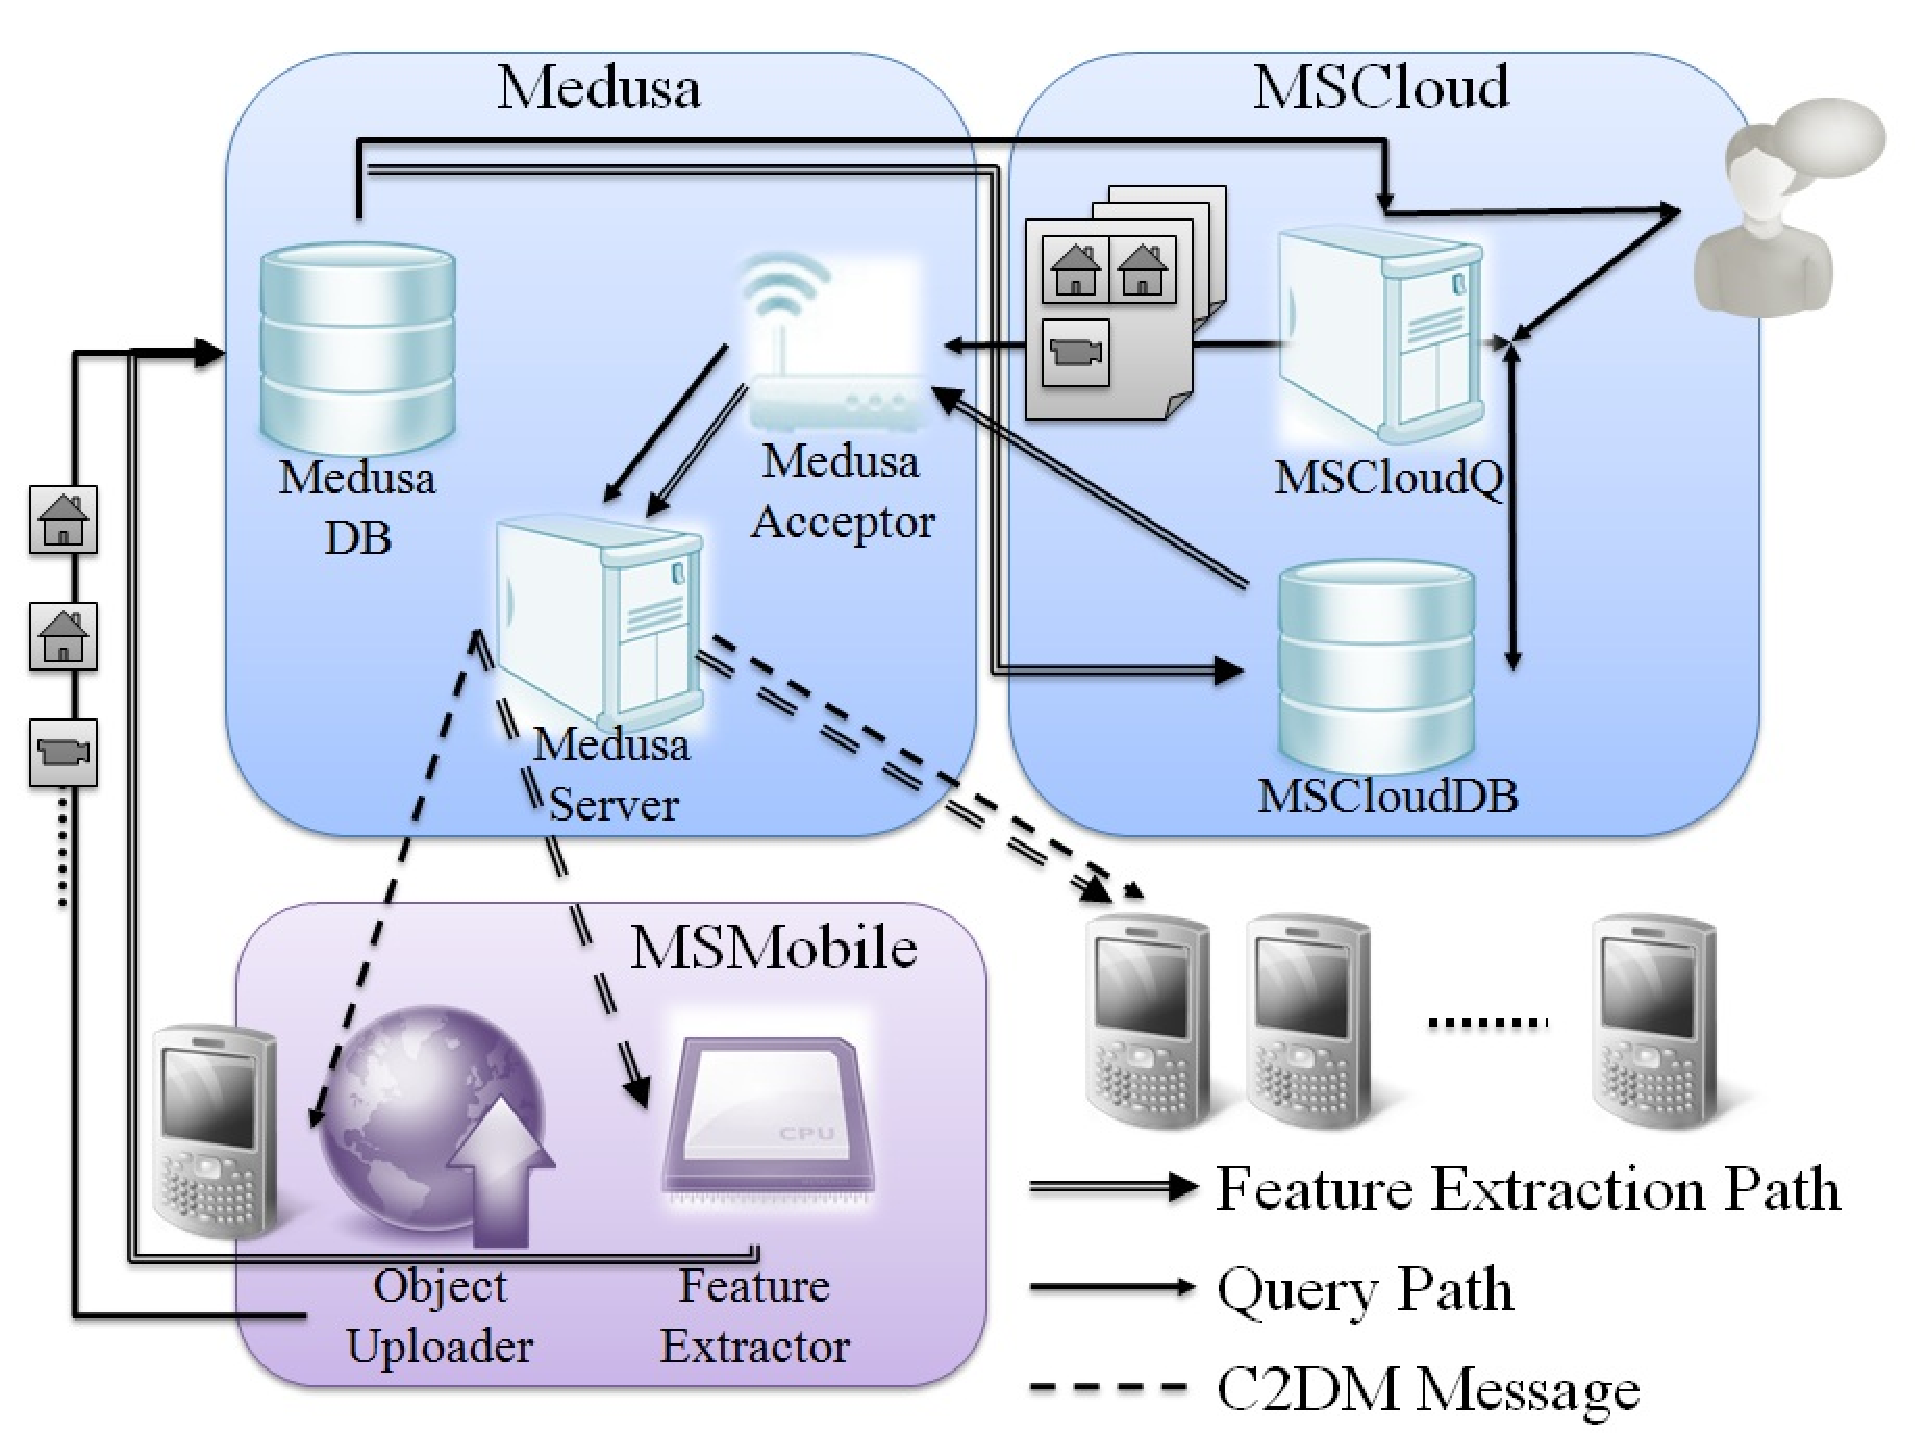
\epsfig{file=pics/architecture.eps,width=0.96\linewidth}
    \end{center}
%    \vspace{-6mm}
    \caption{System Architecture Work Flow}
%    \vspace{-6mm}
    \label{fig:architecture}
  \end{minipage}
  \begin{minipage}{0.32\linewidth}
      \begin{center}
        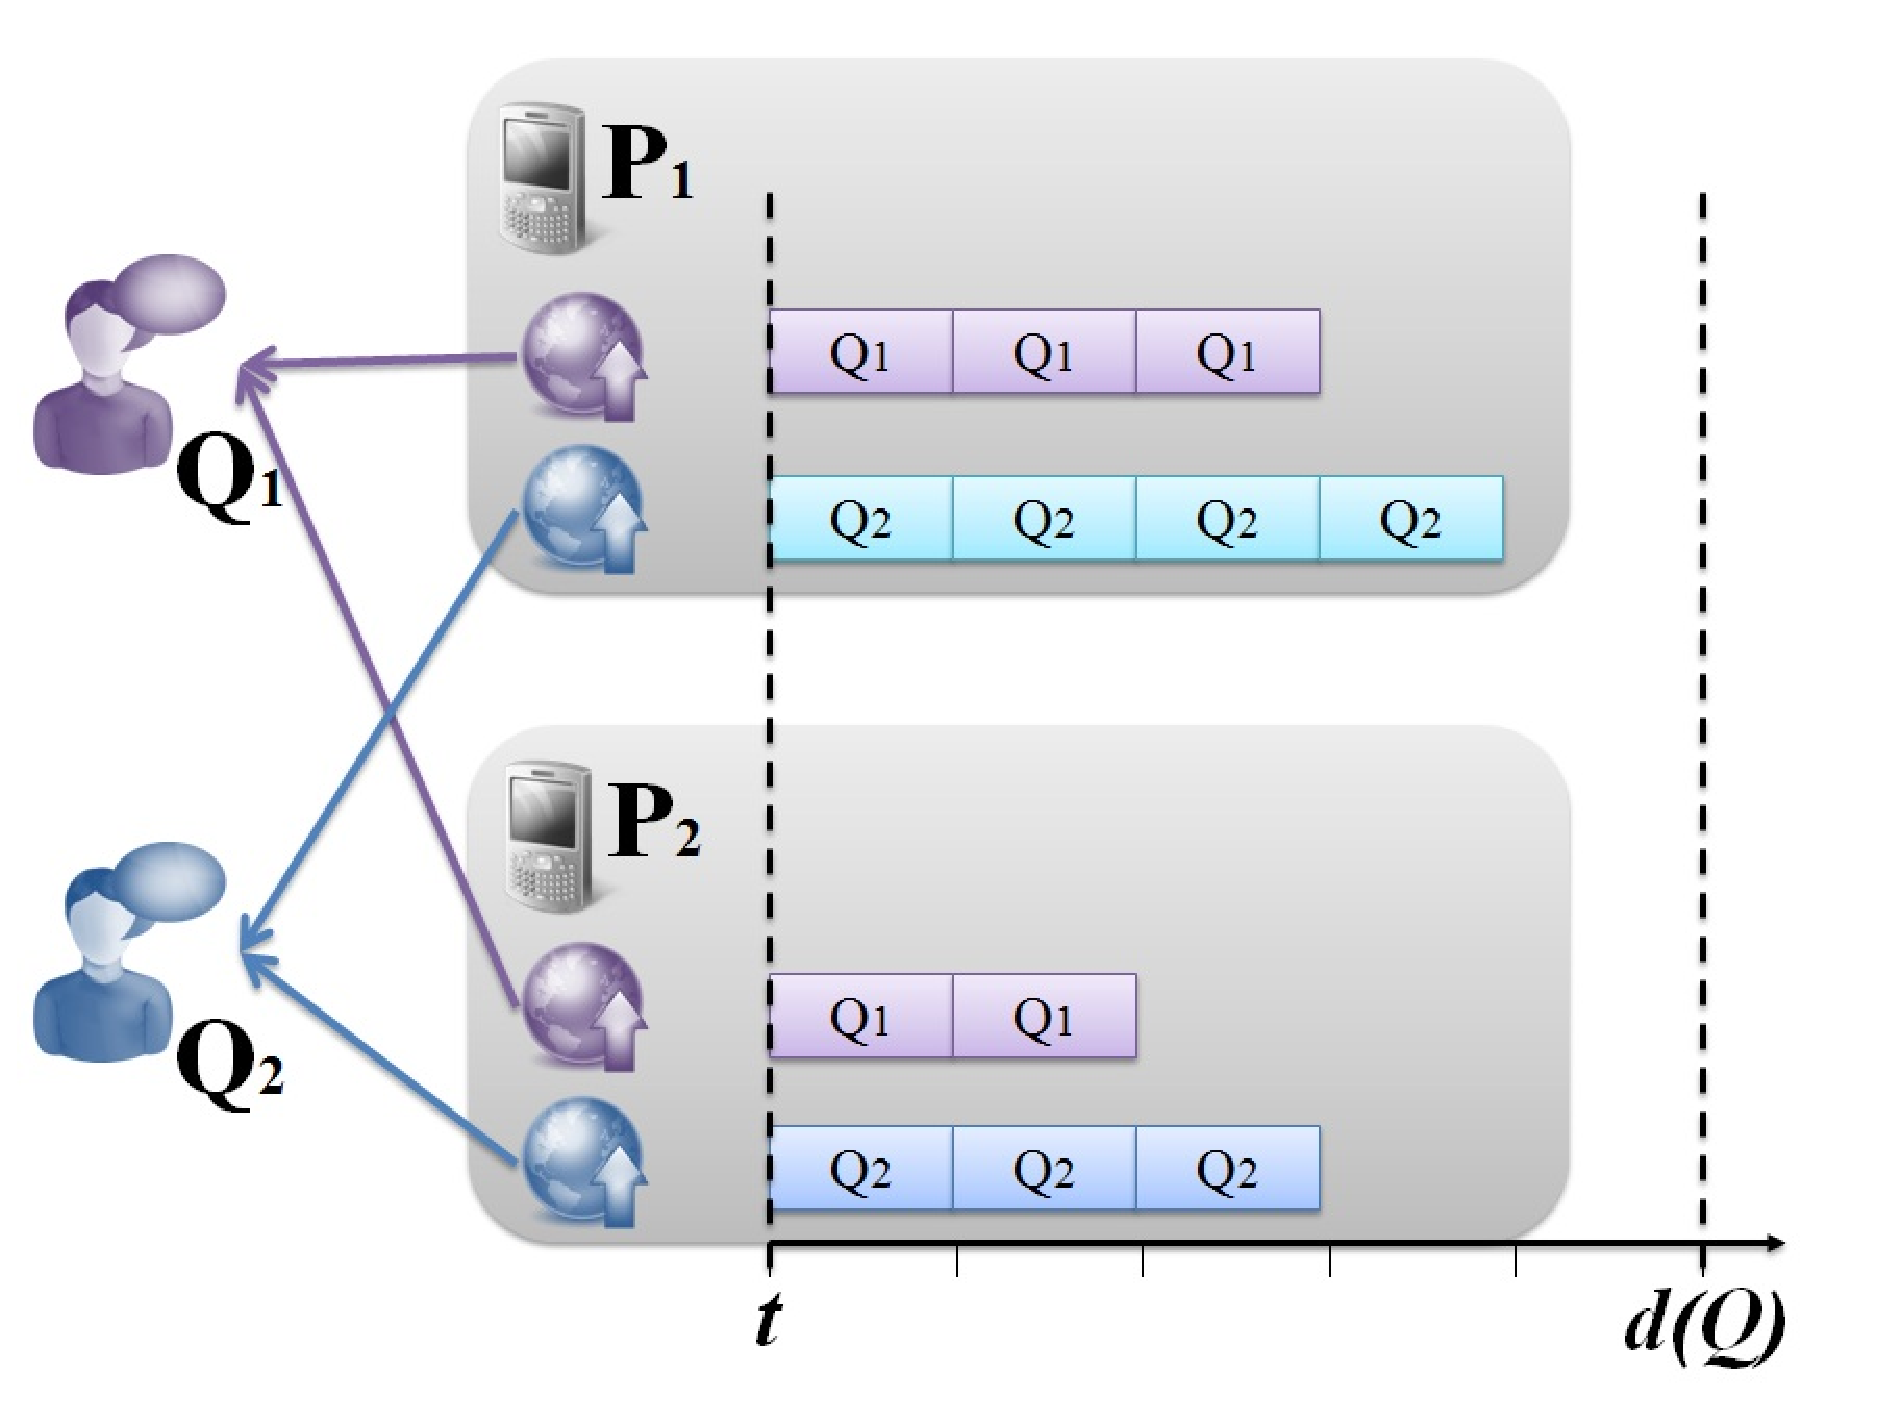
\epsfig{file=pics/example.eps,width=0.96\linewidth}
      \end{center}
%      \vspace{-6mm}
      \caption{Illustration of Concurrent Queries}
%      \vspace{-6mm}
      \label{fig:example}
    \end{minipage}
\end{figure*}

MediaScope is a system that supports timely similarity-based queries
on media objects stored on mobile devices.
%
We begin by describing the MediaScope architecture and then discuss
the design and implementation of each component.

%\vspace*{-0.75ex}
\subsection{Architecture and Overview}
\label{sec-3-1}

Mediascope is conceptually partitioned across a cloud component called
MSCloud, and another component called MSMobile that runs on mobile devices.
%
This partitioned design leverages the computation and storage in
clouds to support geometric queries on the feature space; mobile
devices provide sensing and storage for media objects.

These components interact as follows (Figure~\ref{fig:architecture}).
%
Whenever participants take photos or videos, the \emph{Feature
  Extractor} component of MSMobile continuously extracts, in the
background, image and video features and uploads them to the
\emph{MSCloudDB}.
%
Users (e.g., a security officer or a sportswriter) pose queries to MSCloud
using a standard web interface, possibly on a mobile device.
%
These queries are processed by the \emph{MSCloudQ} query processing
engine, which uses the features stored in the MSCloudDB to compute the
query results.
%
The results of the queries identify the media objects that need to be
retrieved from individual mobile devices.
%
In some cases, a media object may already have been retrieved as a
result of an earlier query; query results are also \emph{cached} in
MSCloudDB in order to optimize retrieval.
%
MSCloudQ coordinates with an \emph{Object Uploader} component on
MSMobile in order to retrieve query results.
%
\camera{Once a query's timeliness bound expires, MSCloudQ terminates
  the corresponding Object Uploader and returns retrieved results.}

MediaScope uses a publicly available crowd sensing platform called
Medusa~\cite{Medusa}.
%
Medusa was originally designed to permit human users to pose
crowd-sensing tasks.
%
MediaScope's retrieval of features and media objects from mobile
devices leverages Medusa's support for ``sensing'' stored information
on these devices.
%
To enable programmed interaction between MSCloud and Medusa, and to
support MediaScope's timeliness requirements, we made several
modifications to the Medusa platform (discussed later).

MediaScope thus provides a high-level abstraction (queries on media
objects) that hides many of the details of object retrieval from
users.
%
In the following subsections, we describe the two most challenging
aspects of MediaScope design: \emph{support for concurrent queries},
a functionality distributed between the MSCloudQ and the Object
Uploader; and \emph{feature extraction}.
%
We conclude with a brief description of other design and
implementation issues.

% First, on MSMobile, there is media file observer which stores all existing media objects (photos and videos)'s general metadata, periodically, MSMobile will execute a media object feature generation task, which compute the feature vectors for each media object, and uploads them to MSCloud. One advantage is that through this way, we avoid the uploading of original media files, which will significantly save the users' bandwidth, e.g. in our implementation, generally one image's original size is about 1.5MB, but the feature data we need to upload is only 54B, for a high definition 30s video taken by Galaxy SIII is about 63M, we only need to upload less than 10 features of the video which is only 540B. Second advantage is that, with a same feature extraction algrithm on the phone as on the cloud, we won't loss any accuracy of these feature metadata.

% Second, interface to commander is clean and concise. Commanders pose search queries of their interest, through the interface to interact with MSCloud. The rest of all the work is left to MSCloud, which will complete all necessarily processing and tasks in the background. MSCloud has two components.
% \begin{itemize}
% \item \textbf{MSCloudDB}: First, Media objects' features uploaded from phones are stored here. It is able to support multiple phones concurrent uploading features at same time, as well as multiple queries concurrent data retrieval. Second, queries' results (original media files) uploaded from phones are also stored here. Since we want to reuse already uploaded media files, MSCloudDB also support media feature data realtime update.
% \item \textbf{MSCloudQ}: MSCloudQ is the query processing engine on the cloud, which includes:
% \begin{itemize}
% \item Interface to Commander. Commander is not necessary to understand the background mechanisms, we provide a detailed query type explaination and straghtforward parameter options for commander. Once the deadline hits or resources are ready, it will pick up the corresponding media files from MSCloudDB, and respond to commander.
% \item Query resolver, and query algorithm execution. Its job is to understand the query objective and parameters, retrieve the data from MSCloudDB, pass them to query optimizer, which will consider all the reality situation and available resources, output the need-to-upload list for each involved users.
% \item Interaction with Phones. After receiving the upload list from query optimizer, MSCloudQ will write task script for each phone, including the uploading scheme parameters, and wait the task execution results from the phone. This part is aware of the deadline of the query, so it will automatically notify the front end interface the file locations, as well as the task termination on the phone.
% \end{itemize}
% \end{itemize}

% Third, MSMobile will accept task notifications from MSCloudQ with task desciption, which are all quite lightweight, usually less than 1Kbytes. MSMobile has its own file uploading scheme, called \emph{maximum credit scheme}, we will discuss it in detail in following.



% In summary, our system work flow is shown in Figure~\ref{fig:architecture} (will be modified to new architecture image).
%%

%\vspace*{-0.75ex}
\subsection{Design: Concurrent Queries}
\label{sec-3-2}

The most challenging component of MediaScope is support for concurrent
queries~---~\camera{MSCloudQ may receive one or more queries while
  other queries are being processed.}
%
In MediaScope, the result of a query is a list of media objects to be
retrieved from a subset of the participating phones.
%
Recall that each query has a timeliness constraint.
%
In the presence of concurrent queries, MediaScope may need to upload
all media objects before their timeliness bound expires.
%
In general, this may be difficult to achieve because \camera{wireless
bandwidth can vary significantly over time, resulting in variable
upload times for images.}

To illustrate this, consider the example of two concurrent queries
$Q_1$ and $Q_2$ that arrive at the same time for media objects
distributed across two phones $P_1$ and $P_2$ in Figure~\ref{fig:example}.
%
Also, assume that both queries have a timeliness bound of 5 seconds,
each object can upload 1 object per second, and all objects are of the
same size.
%
If $Q_1$ needs to retrieve 3 objects from $P_1$ and 2 objects from
$P_2$, while $Q_2$ needs to retrieve 4 objects from $P_1$ and 3 from
$P_2$.
%
Under these circumstances, it is not possible to satisfy the
timeliness requirements of
%\xing{both?} No, there exists a schedule by which either q1 or q2 can
%be satisfied, but not both
one of the two queries.
%
In practice, the problem is much harder because there may be more than
two concurrent queries, many more participating devices, queries can
arrive at different times, media objects may have different sizes, and
wireless available bandwidth can vary dynamically.
%
Especially because of the last reason, \camera{admission control
  cannot guarantee that all timeliness constraints are met, or may
  severely underutilize the available bandwidth}.

MediaScope uses a different approach, \emph{trading off query
  completeness for timeliness}.
%
In MediaScope, not all query results may be uploaded within the
timeliness bound, but the challenge is to upload the most relevant
queries so as to maximize the amount of \emph{information} retrieved.
%
In doing this, there are two challenges: how to differentiate between
queries, and how to prioritize media items for the retrieval in order
to maximize the information retrieved.

% In this case, our goal is to attempt to maximize the amount of
% information delivered across all queries. In particular, this means
% that it would be preferable to obtain as much of the ``high order bits''
% of the query result for each query, than to obtain all of the results
% for one query.

MediaScope addresses these two challenges using a \emph{credit
  assignment} mechanism.
%
Each query is assigned, by MediaScope, a number of credits.
%
The credits assigned to a query reflect the importance of that query
and result in proportionally more information being uploaded for that
query (and therefore the proportional completeness of the query result).
%
The specific credit assignment mechanism for queries is beyond the
scope of this paper, but MediaScope may use monetary incentives (e.g.,
users who pay more get more credits \camera{for their queries}) or other
approaches in order to assign credits to queries.

If a query is assigned $n$ credits, it divides up these credits among
its results (media objects) in a way that reflects the importance of
each object to the query.
%
The key intuition here is that, for a given query, \camera{\emph{the
  importance of a result object to the query can be determined by the
  feature space geometry}}.
%
For example, consider a query $Q$ which attempts to retrieve the two
nearest photos in feature space to a given photo $c$.
%
If the resulting photos $a$ and $b$ are each 20 units and 80 units
distant from $c$ in feature space, and $Q$ has been assigned 100
credits, $a$ and $b$ each receive 80 and 20 credits respectively (in
inverse proportion to their distances to $c$).
%

MediaScope uses this intuition to define credit assignment to result
objects.
%
Once objects have been assigned credits, object uploading is
prioritized by credit in order to maximize the total credit retrieved
across all concurrent queries.
%
In what follows, we first describe the queries that MediaScope
supports and how credits are assigned for each query.
%
We then describe MediaScope's credit-based object scheduling technique
and discuss its optimality.

% Our approach uses two mechanisms to address this challenge:
% \begin{itemize}
% \item a system defined assignment of ``credits'' to individual queries: this
%   assignment roughly determines the relative proportion of resources
%   that this query can use, that is, any query $Q_i$ has been assigned the credits $c(Q_i)$.
% \item for each query, we also define a method by which credits can be
%   allocated to query results and design a scheduling algorithm that
%   attempts to maximize the total number of credits retrieved. For example, $n$ objects best answers query $Q_i$, namely $Q_i=\{o_i^1, o_i^2, \cdots, o_i^n\}$, we assign $n$ objects with credits $c(o_i^1), c(o_i^2), \cdots, c(o_i^n)$ and satisfy $c(Q_i)=\sum_{o\in Q_i} c(o)$
% \end{itemize}

% Thus, query semantics are ``approximate'' necessarily because of
% timeliness constraints one may not get complete queries; level of
% completeness can be varied by adjusting the credits assigned to each query.

%\vspace*{-0.75ex}
\subsubsection{Queries and Credit Assignment}
\label{sec-3-2-1}

Our current instantiation of MediaScope supports three qualitatively
different queries: nearest neighbor, clusters, and spanners.
%
Below, we discuss the design of the query engine MSCloudQ and how
credits are assigned to query results.
%
Recall that for each query, users can specify time, location and
freshness attributes: before performing each of the queries described
below, MSCloudQ filters all the feature vectors stored in MSCloudDB to
select feature vectors that match these attributes.
%
In our description of the queries below, we assume that this filtering
step has been applied.

% We are supporting four queries from the discussion of \ref{sec-2-2}.
% %
% In order to fullfill different query requirement, we design specified
% algorithms for each query that best coordinate the idea of the query.
% %
% Algorithm for each different query not only generates a list of media
% objects to upload, but each media object is associated with a credit,
% indicating the “importance” of such object.
% %

% We introduces the design for different queries, each query is associated with two steps: first, query optimization(algorithm execution), second, credit assignment.

\mypar{k-Nearest Neighbors.}
%
For this query, the user supplies a \emph{target} image and the server
attempts to return the $k$ nearest images (from photos or videos) in
feature space to the target.
%
The implementation of this query is straightforward: it is possible to
build indexes to optimize the search for the $K$ nearest neighbors,
but our current implementation uses a brute force approach.

% \textbf{Step 1}: The algorithm for this query is quite straghtforward, MSCloudQ first filters out those not qualified metadata from MSCloudDB, and returns qualified media metadata, \emph{Top K algorithm} iterates over all qualified feature data, calculate the given image's feature similarity to those from MSCloudDB, and returns Top K similar objects' IDs to MSCloudQ.

Credit assignment for this query attempts to capture the relative
importance of the query results.
%
Thus, the assignment of credits to each result is proportional to its
similarity to the target image.
%
For the $i$-th result, let $s_i$ be the similarity measure to the
target; we then assign credits to the $i$-th result proportional to
$p_i = (1 - \frac{s_i}{\sum{s_i}})$.

%
% So our assigning scheme is to assign credit proportional to the
% similarity to the original given image.
% %
% Specifically, take similarity value for each object from the intended
% object, denote as $s_{i}$, the smaller $s_i$, the more similar, so the
% portion is
%

\mypar{$K$ Clustering.}
%
The second class of queries supported by MSCloudQ is based on
clustering in feature space.
%
This query takes as input the number $k$ as well as well as a
\emph{type} parameter which describes the expected result and can have
one of two values:
\begin{description}
\item[Cluster Representative] With this parameter, the result contains
  $k$ images, one from each cluster. For each cluster, our algorithm
  selects that image as the representative whose distance is least to
  the centroid of the cluster. Intuitively, this query type identifies
  different ``topics'' among images taken by participating users.
\item[Common Interest] With this parameter, the result includes images
  from that cluster which contains objects belonging to the most
  number of users. Thus, if the $i$-th cluster contains images from
  $u_i$ users, the query returns images from that cluster for which
  $u_i$ is the largest. Intuitively, this query identifies the cluster
  that represents the maximal common interest between participating
  users. Within the selected cluster, the query returns one image for
  each participating user, selecting that image of the user that is
  closest to the centroid of the cluster.
\end{description}
%
These queries can be implemented by any standard algorithm for
$k$-means clustering.

For the \emph{cluster representative} type of query, we assign credits
proportional to the size of the cluster.
%
Thus, if the $j$-th cluster's size is $c_j$, the credit assigned to
the image selected from cluster $j$ is proportional to $\frac{c_j}{\sum{c_j}}$.

For the \emph{common interest} type of query, we assign a credit to
each selected image that is inversely proportional to the image's
distance from the centroid of the cluster.
%
The credit assignment is similar to $k$ nearest neighbors above.

% Second query we proposed is \emph{K Representative Objects} , with which, people can find out K most representative objects over the whole database.

% \textbf{Step 1}: We tried few algorithms for  \emph{K Representative Objects} Query. The way we evaluation the algorithm performance is that we manually took around 200 photos in 5 different scenes of 5 different locations with Galaxy SIII, manually marked those 200 photos into 5 clusters. Then we apply different clustering algorithm on the dataset, and compare the results with manually marked clusters. We found that \emph{KMeans} clustering performs best with an average less than 2 error photo classification  per cluster. So the final algorithm we adopted for this query is  K-Means algorithm. After retrieving related feature data from MSCloudDB, we use Kmeans to classify the all qualified objects to $K$ clusters, and select one object from each cluster under the condition that the object is most close(similar) to its cluster center.

% \textbf{Step 2}: The concept of credit assigment here is a little different from previous query, similarity here is not a good metric anymore, since only one object is selected in each cluster. We proposed the cluster size metric which indicates that the larger a cluster, the more credit the representative object should get.  So consider cluster $i$'s size $cs_i$, the credit portion for cluster $i$ is $\frac{cs_i}{\sum{cs_i}}$ and assign credit according to the proportion.

% Third query we proposed is \emph{Common Interest Objects}: people might want know others' common interest, e.g. most people tend to  take photos or videos of some sightseeing, like beach, ocean, if most people has such interest, we can point it out and show these photos or videos to commander.

% \textbf{Step 1}: The algorithm here is same as \emph{K representative objective} query, we use KMeans to clusters qualified features to $K$ clusters(we predefined the parameter $K= 6$ in the algrithm, commander is free to assign or not ). The difference compared to previous query is that we will select the cluster with most different users, if multiple clusters have same number of users involved, we use number of objects as another criteria. We will return the objects in selected cluster.

% \textbf{Step 2}: Here, our idea for credit assigment is that more close to cluster center, more credit it should get, we assign like this is because those close to center objects contains more information compared to those who are far from center. The rest is identical to the algorithm in \emph{Top K Objects} Query.

\ifdefined\notdef
\mypar{Spanner.}
%
The third query that MediaScope supports is based on spanning the
feature space.
%
The intuition behind the query is to return a collections of images
which \emph{span} the feature space.

% Forth query in our system is \emph{Spanner: Most distinct object Set}, the intuition behind this query is that commander may be interested in the total information contained by the available data. To select a set of media objects that contains most information requires those objects to be quite distinct to each other. So for this query, we first defined in a rigorous mathematical way, and give a suboptimal algorithm to the problem.

MSCloudQ uses a maximum weighted spanning tree algorithm in order to
select results for this query; it attempts to find the most dissimilar
pairs of objects from each participating user, while constraining the
number of images selected from each user to a nominal ``budget''.
%
Assume that $K_n$, the complete graph on $n$ vertices (vertices
represent objects), has a vertex set $V$ which is partitioned into $C$
classes $V_{1},\ldots,V_{C}$ (classes represent users).
%
Let $v_{i_t}$ denote vertex $i$ in class $V_t$.
%
Let $e_{i_t j_k}$ represent the edge connecting $v_{i_t}$ with
$v_{j_k}$.
%
Assume edge $e_{i_tj_k}$ has weight $w_{i_tj_k}$ (where the weight
represents the dissimilarity between objects $i_t$ and $j_k$).
%
Furthermore, assume vertex $i_t$ has size $s_{i_t}$ (size of object
$i_t$), and class $j$ has capacity $b_j$ (total size that can be
uploaded from user $j$).
%

The objective is to find a spanning tree of maximum weight on a vertex
subset which respects the class size constraints.
%In this case, we can easily prove that the added edge value decreases with adding order.
%The physical meaning behind this objective is that the
%selected points are as distinct to each other as possible.
This objective selects objects which are dissimilar from one
another.
%
Here is the integer program for this problem:

{\footnotesize
\begin{align}
\max        & \notag
              \sum_{i_t< j_k} w_{i_tj_k} y_{i_tj_k} \\
\text{s.t.     } & \label{con:ineq1}
              y_{i_tj_k} \leq x_{i_t}             & \forall i_t\neq j_k \\
            & \label{con:ineq2}
              y_{i_tj_k} \leq x_{j_k}             & \forall i_t\neq j_k\\
            & \label{con:ineq4}
            \sum_{i_t\in V_t} s_{i_t}x_{i_t}\le b_t        & \forall t=1,\ldots , C \\
            & \label{con:ineq5}
            \sum_{i_t<j_k} y_{i_tj_k}=\sum x_{i_t}-1      &    \\
             & \label{con:ineq6}
            \sum_{i_t<j_k} y_{i_tj_k}\le |S|-1           & \forall S\subset V, S\neq \emptyset\\
            & \notag
            x_{i_t} \in\{0,1\}        & \forall i_t\\
            & \notag
            y_{i_tj_k} \in\{0,1\}                 & \forall i_t\neq j_k
\end{align}
}

In this integer program, variable $x_{i_t}$ is used as the indicator
variable for selecting vertex $v_{i_t}$.
%
Similarly, variable $y_{i_tj_k}$ is used as the indicator variable for
selecting edge $e_{i_tj_k}$.
%
Inequality \ref{con:ineq1} and \ref{con:ineq2} ensure that edge
$e_{i_tj_k}$ is not selected if either vertex $i_t$ or $j_k$ is not
selected.
%
Inequality \ref{con:ineq4} ensures that the total size of vertices
chosen from class $V_i$ does not exceed $b_i$.
%
Denotation \ref{con:ineq5} and \ref{con:ineq6} ensures that a maximum
spanning tree is selected.
%
Since the above problem is NP-hard, we use a $O(N^2log(N)^2)$
heuristic (Algorithm~\ref{alg:mst}).
%

For this query, intuitively, credit assignment should give more
importance to dissimilar images.
%
For the $i$ query result, we compute $d_i$, the average distance from
the $i$-th image to all other images.
%
The credit assigned to this image is proportional to
$\frac{d_i}{\sum{d_i}}$. %\ramesh{Please check.}\jyr{I didn't find problem here}

% \textbf{Step 2}: From the above algorithm we get a set of media objects that most dissimilar to each other. Our design for the credit assignment is that take average similarity to all other selected objects as the metric for each objects, say for object $i$ that average similarity to other objects is $avgsim_i$, and its credit portion is $\frac{avgsim_i}{\sum{avgsim_i}}$ the credit assignment is according to the portion. The meaning for this assigment is that those who are farest from others need more credit because it contains the information that might quite independent to others.

% Algorithm for each different query not only generates a list of
% media objects to upload, but each media object is associated with a
% credit, indicating the ``importance'' of such object. We can
% evaluate each query's result as the total credits of uploaded media
% objects.

\fi

\mypar{Spanner.}
%
The third, and qualitatively different query that MediaScope supports
is based on spanning the feature space.
%
The intuition behind the query is to return a collection of images
which \emph{span} the feature space.
%
In computing the spanner, we assume that each user $t$ contributes
exactly $s_t$ images, where $s_t$ is derived from the query's
timeliness bound and a nominal estimate of the average upload rate
from the corresponding mobile device\footnote{ \camera{As we describe
    later, the average upload rate is estimated dynamically by MSCloudQ.}}
%
Our spanner maximizes the minimum dissimilarity between all pairs.
%
% Each user has a collection of relevant images.  The commander would like to receive all relevant images from each user, but due to deadline constraints, this is not feasible.  Therefore, we assume that user $t$ uploads exactly $s_t$ images.  Each pair of images has a dissimilarity metric associated with it.  The commander would like to receive a subset of images, which maximizes the minimum dissimilarity between all pairs, with the intuition that such an objective returns a collection of photos which span the feature space.

We now express this problem mathematically.
%
Assume that $K_n$, the complete graph on $n$ vertices (vertices
represent images), has a vertex set $V$ partitioned into $C$ classes
$V_{1},\ldots,V_{C}$ (classes represent users).
%
Let $v_{i_t}$ denote vertex $i$ in class $V_t$.
%
Let $e_{i_t j_k}$ represent the edge connecting $v_{i_t}$ with
$v_{j_k}$.
%
Assume edge $e_{i_tj_k}$ has weight $w_{i_tj_k}$ (where the weight
represents the dissimilarity between objects $i_t$ and $j_k$).

Assuming that exactly $s_t$ vertices must be selected from $V_t$, we
need to select a set of vertices so that the minimum edge weight of
the selected clique is maximized.
%
This problem can be formulated as a mixed-integer program: % (general we
% find that all files are roughly the same, so \emph{WLOG} we assumption
% that all file size equal to 1):
%
%\vspace{-5mm}
\begin{align} \footnotesize
\textbf{$\max$}        & \notag
             \   z \\
\text{s.t.     }&\label{con:min}
             z\le w_{i_tj_k} y_{i_tj_k}           & \forall i_t,j_k \ s.t.\  i_t<j_k\\
            & \label{con:ineqx1}
              y_{i_tj_k} \leq x_{i_t}             & \forall i_t,j_k \ s.t.\ i_t<j_k \\
            & \label{con:ineqx2}
              y_{i_tj_k} \leq x_{j_k}             & \forall i_t,j_k \ s.t.\ i_t<j_k\\
            & \label{con:ineqx3}
            x_{i_t}+x_{j_k}-y_{i_tj_k}\le 1     & \forall i_t,j_k \  s.t.\ i_t<j_k\\
            & \label{con:ineqx4}
            \sum_{i_t\in V_t} x_{i_t}= s_t        & \forall t=1,\ldots , C \\
            & \notag
            x_{i_t} \in\{0,1\}        & \forall i_t\\
            & \notag
            y_{i_tj_k} \in\{0,1\}                 & \forall i_t,j_k \  s.t.\ i_t < j_k
\end{align}
%\vspace{-4mm}

In this mixed-integer program, variable $x_{i_t}$ is used as the
indicator variable for selecting vertex $v_{i_t}$ for the clique.
%
Similarly, variable $y_{i_tj_k}$ is used as the indicator variable for
selecting edge $e_{i_tj_k}$ for the clique.
%
Variable $z$ is used to achieve the $\min_{i_t<j_k}{w_{i_tj_k}
y_{i_tj_k} }$.
%
Inequalities \ref{con:ineqx1} and \ref{con:ineqx2} ensure that edge
$e_{i_tj_k}$ is not selected if either vertex $i_t$ or $j_k$ is not
selected.
%
Inequality \ref{con:ineqx3} guarantees that $y_{i_tj_k}$ is
selected if both vertices $i_t$ and $j_k$ are selected.
%
Inequality \ref{con:ineqx4} ensures that the number of vertices
selected from class $t$ is $s_t$.
%

The above problem is NP-hard so we use a $O(|V|^2)$ heuristic
(Algorithm~\ref{alg:mst}) for solution.
%
The idea behind this heuristic is to select the set of vertices
greedily i.e., add ``qualified'' vertices whose minimum weighted edge
to the set selected thus far is maximum.
%
``Qualified'' vertices are vertices in the classes which have not yet
met their constraint, and hence these vertices can still be selected.
%
%
We deal with the issue of which vertex should be selected first by
trying all possible vertices as being the first vertex in the set and
taking the maximal such set.
%

\begin{algorithm}[H]
\caption{: \textsc{MaxMin Heuristic}} \label{alg:mst}
\begin{small}
\begin{algorithmic}[1]
\STATE Define a list $l$ for storing best vertex set and a variable $max\_min$ for minimum weighted edge
\STATE $l\leftarrow []$, $max\_min \leftarrow 0$
\FORALL{ $i\in\{1,\ldots,V\}$}
        \STATE $min=\infty$
        \STATE Define a temporary list $l_t$ and $l_t \leftarrow i$
        \WHILE {new item added to $l_t$}
            %\STATE initialize an empty list $Temp_L$
            \FOR {$j \in\{1,\ldots,V\}$ and $j \not \in L$}
                %\STATE compute $j$ minimum similarity distance $msd_j$ to vertices in $LT$, and add $[msd_j, j]$ to $Temp_L$
                \STATE $d(j) \leftarrow \min_{o \in l_t} similarity\_dist(o,j)$
            \ENDFOR
            \IF{ $\exists$ qualified vertex $v$ }
                \STATE $l_t.add(\{v | \max {d(v)}\})$
                \STATE  $temp\_min\leftarrow d(\{v | \max {d(v)}\})$
            \ENDIF
        \IF{ $temp\_min < min$}
            \STATE $min = temp\_min$
        \ENDIF
        \ENDWHILE
        \IF{$min>max\_min$}
                \STATE $max\_min=min$
                \STATE $l=l_t$
        \ENDIF
\ENDFOR
\end{algorithmic}
\end{small}
$\textbf{OUTPUT}$: $l$ and $max\_min$
\end{algorithm}

For this query, intuitively, credit assignment should give more
importance to dissimilar images.
%
For the $i$-th query result, we compute $d_i$, the average distance from
the $i$-th image to all other images.
%
The credit assigned to this image is proportional to
$\frac{d_i}{\sum{d_i}}$.

\mypar{Extensibility of MSCloudQ.}
%
These are, of course, not the only kinds of geometric queries that can
be supported.
%
Developers wishing to extend MSCloudQ by adding new queries can do so
quite easily by: (a) defining the query syntax and semantics, (b)
implementing the query algorithm, and (c) specifying a proportional
credit assignment based on the semantics of the query.

% \begin{algorithm}[H]
% \caption{: \textsc{MST Heuristic}} \label{alg:mst}
% \begin{small}
% \begin{algorithmic}[1]
% \STATE Define a list $l$ for storing tree and a variable $opt\_sum\_mst$ for minimum-spanning-tree(MST) edge sum
% \STATE $l\leftarrow []$, $opt\_sum\_mst \leftarrow 0$
% \FORALL{ $i\in\{1,\ldots,V\}$}
%         \STATE {Define a temporary list $l_t$ and $l_t \leftarrow i$}
%         \WHILE {New vertice added to $l_t$}
% %            \STATE Define hashmap $hm$ and $hm \leftarrow \emptyset $
%             \FOR {$j \in\{1,\ldots,V\ and \  j  \not \in l_t$}
% %                \STATE Compute $j$'s minimum similarity distance $msd_j$ to vertices in $l_t$, $hm.add[msd_j, j]$
%                 \STATE $d(j) \leftarrow \min_{o \in l_t} similarity\_dist(o,j)$
%             \ENDFOR
%             %\STATE Desend sort $hm$
%             \IF{ $\exists$ qualified vertice $v$ }
%                 \STATE $l_t.add(\{v | \max {d(v)}\})$
%             \ENDIF
%         \ENDWHILE
%         \STATE Compute MST for vertices in $l_t$, and compute edge sum of MST $sum\_mst$
%         \IF{ $sum\_mst > opt\_sum\_mst$}
%             \STATE $l\leftarrow l_t$ and $opt\_sum\_mst = sum\_mst$
%         \ENDIF
% \ENDFOR
% \end{algorithmic}
% \end{small}
% $\textbf{OUTPUT}$: $l$ and $opt\_sum\_mst$
% \end{algorithm}


% We currently developed four sample queries in our system frameworks as discussed above. Our system is a complete and extensible framework that opens most APIs to developers, by which they can easily improve or change the scheme we used in the system as well as add new interesting queries to the system.

% For the system extension, developers are able to integrate \mscope in addition to the social apps, people is able to know friends' willing-to-share media content actively, besides, since some query design are NP-hard, developers can improve the system performance with other closer optimal algorithms.

% For Query Extension,  we offers neat APIs for advanced developers to design their own interested queries. Developer only need to set their optimization goal here, and combine or design their algorithm for the query, system libraries provides some popular algorithm implementation, like Centroid-based clustering,  Distribution-based clustering, Top K Selection, Minimum Spanning Tree, etc. System provides standard api to interact with MSCloudDB, the developers only need to use the API to retrieve metadata for their optimization function, and pass the output to MSCloudQ, that's all set for query design part. Another part of query extension is the credit assignment scheme for new query results. A constant $TOTAL_CREDIT$ is predefined in system library, the things left to developer is the way to assign the credit to the query algorithm output and pss to MSCloudQ's $Credit_Evaluation()$, general rule for credit assignment is higher credit, high uploading priority. After the above two steps, new query is ready to use from MSCloudQ's user interface.

%\vspace*{-0.75ex}
\subsubsection{Credit-based Scheduling}

In general, users can pose concurrent queries to MSCloudQ.
%
Queries may arrive at different times and may overlap to different
extents (we say one query overlaps with another when one arrives while
the other's results are being retrieved).
%
Furthermore, different queries may have different timeliness
constraints, may retrieve different numbers of objects (e.g., for
different values of $k$, or different sizes of spanners), and  the
retrieved media objects may be of different sizes (images with
different resolutions).
%
In these cases, MSCloudQ needs an algorithm that schedules the
retrieval of different objects subject to some desired goal.

In MediaScope, this goal is to maximize the total completeness of
queries, defined as the sum of the credits of all the uploaded images.
%
To achieve this, recall that MSCloudQ assigns a credit budget to each
query based on the importance of that query; then, using the
proportions defined above, it assigns credit values to each query
result.

% values to selected media objects, such credits assignment can help
% evaluate the completeness of one query.
% %
% For each query we can observe how many credits are uploaded to
% MSCloudQ within their timeliness constraint.
%

To mathematically define the completeness goal, we first introduce
some notation.
%
Let $Q_i$ denote the set of media objects that form the result of the
$i$-th query, and let that query's timeliness constraint be $d(Q_i)$.
%
Let $g(o)$ be an indicator variable that denotes whether a media
object $o$ is retrieved before $d(Q_i)$.
%
Then, for the $i$-th query, the total credit for all uploaded media
objects is given by: $$g(Q_i)=\sum_{o\in Q_i}g(o)\cdot c(o)$$
%


\begin{figure*}[t]
\centering
\subfigure[Average CEDD Execution Time Per Image for Different Size]{
\includegraphics[width = 5.6cm]{pics/cedd.eps}
\label{fig:resize_1}}
    \hfil
\centering
\subfigure[Average Time of Resizing image to Different Size]{\includegraphics[width = 5.6cm]{pics/resize.eps}
\label{fig:resize_2}}
    \hfil
\centering
\subfigure[Average Error Rate of KMeans Clustering for Different Size]{\includegraphics[width = 5.6cm]{pics/kmeans.eps}
\label{fig:resize_3}}
\caption{Image Resizing Overhead and Tradeoffs}
\label{fig:resize}
\end{figure*}


Thus, given a series of concurrent queries $\mathbb{Q}$, the total
number of credits retrieved is given by:
%
$$c(\mathbb{Q})=\sum_{Q\in \mathbb{Q}}\sum_{o\in Q}g(o)\cdot c(o)$$
%
Maximizing this quantity is the objective of MediaScope's retrieval
scheduling algorithm.

It turns out that it is possible to decompose this objective into a
per-device \emph{credit maximization scheduling} algorithm.
%
To see why this is so, let $\mathbb{P}$ denote the set of
participating devices, and the $k$-th device be denoted by $p_k$.
%
Then, the above credit sum can be written, for concurrent queries $\mathbb{Q}$:
%
% From participated phones' (denoted as $\mathbb{P}$) perspective, after aggregated assigned media objects for $Q$ of concurrent queries $\mathbb{Q}$, the $i$-th phone $p_i$ uploading list can be denoted by $p_i=\{o_1, o_2, \cdots, o_n\}$ with credits $c(o_1), c(o_2),\cdots,c(o_n)$ and deadlines $d(o_1), d(o_2),\cdots,d(o_n)$. Therefore, for any series of concurrent queries $\mathbb{Q}$, we have:
\begin{align*} \small
c(\mathbb{Q})&=\sum_{Q\in \mathbb{Q}}\sum_{o\in Q}g(o)\cdot c(o)&\\
&=\sum_{Q\in \mathbb{Q}}\sum_{P\in \mathbb{P}}\sum_{o\in P\cap Q}g(o)\cdot c(o)&\\
&=\sum_{P\in \mathbb{P}}\sum_{o\in P}g(o)\cdot c(o)&\\
\end{align*}
%\vspace{-5mm}

This equality shows that, in order to maximize the total credits
retrieved across a set of concurrent queries $c(\mathbb{Q})$, it
suffices to maximize the total credits uploaded by each participating
device: $\sum_{P\in \mathbb{P}}c(P)$.
%
This is true under the following two assumptions:
(a) if two different queries retrieve the same object from $P_k$, then
%object is uploaded only once if it is uploaded at all,
\camera{the object will need to be uploaded at most once} and
(b) the credit assigned to that object is the sum of the credits
allocated by each query to that object.
%

This finding has a nice property from the systems perspective: it
suffices to run a local credit-maximizing scheduler on  each
participating device in order to achieve the overall objective.
% %
% With this property, each phones can make their own best decision of
% uploading objects, i.e., local optima, to achieve the overall optima
% at MSCloudQ side.
% %
% The key advantage of doing this is uploading schedule can be adjust
% freely based on phone's current uploading progress.
%
In general, local schedulers have the attractive property that they
can locally adapt to bandwidth variations without coordinating with
MSCloudQ, and need only minimal coordination with MSCloudQ in order to
deal with new query arrivals.
%
In MediaScope, the Object Uploader component of MSMobile implements
the scheduling algorithm.

% Such adjustment is important because sometimes bandwidth varies a lot
% and incoming queries might largely change the existing uploading
% schedule as well.
% %
% It is inefficient for MSCloudQ to keep updating all phones' progress
% status and communicate with phones to transfer updated schedules.
% %
% Therefore, we decide to implement the scheduling component on MSMobile
% side.
%

\mypar{An Optimal Scheduler.}
%
We first describe a scheduling algorithm that is \emph{optimal} under
the assumption of fixed file sizes and fixed wireless bandwidth per
participating device.
%
Under these assumptions, for each object $o$, it is possible to
compute the exact upload time $t(o)$ which is the same for all
objects.
%
If each object's timeliness bound is $d(o)$ (different objects can have
different bounds), our goal is to find an uploading sequence such
that $\sum_{o} g(o)\cdot c(o)$ is maximized.

First, we may assume that an optimal schedule orders the objects by
earliest timeliness bound first.
%
Assume an optimal schedule does not order objects by earliest
timeliness bound first.
%
Then there exist two objects $i$ and $j$ for which $d(o_i)>d(o_j)$ but $i$
is scheduled before $j$.
%
By switching the order of objects $i$ and $j$ we can obtain
another optimal schedule.
%

However, merely scheduling by earliest timeliness bound is not likely to
maximize credit.
%
To do this, the algorithm preprocesses the schedule to obtain a set of
scheduled objects in the following way.
%
It orders the objects by earliest timeliness bound first.
%
Then, it adds objects to the schedule one right after another as long
as each object's finish time does not exceed the timeliness bound.
%
If an object's end time exceeds its timeliness bound, the algorithm removes
the object receiving the smallest credit of those objects scheduled thus
far (including current object) and shifts objects to the right of this
object to the left by $t(o)$ to cover the gap.
%
Intuitively, this step maximizes the total credit
uploaded: lower credit objects, regardless of the query they belong
to, are replaced.
%
The algorithm then selects the next object in order of timeliness.

\begin{algorithm}[H]
\caption{: \textsc{Optimal Uploading Schedule}} \label{alg:opt}
\begin{small}
\begin{algorithmic}[1]
\STATE Arrange the pending objects list $\mathbb{O}$ by earliest timeliness bound first, scheduling $\mathbb{S}\leftarrow[]$
\STATE $l\leftarrow 0$

\FOR {$o$ $\leftarrow$ $\mathbb{O}.first$}
        \STATE $\mathbb{S}\leftarrow o$
        \STATE $\mathbb{O}.remove(o)$
        \IF {$l+t(o)\le d(o)$}
                \STATE $l\leftarrow l+t(o)$
        \ELSE
                \STATE Remove the smallest credited object in $\mathbb{S}$
                \STATE Shift all objects to the right of this object to left by $t(o)$
        \ENDIF
\ENDFOR
\end{algorithmic}
\end{small}
$\textbf{OUTPUT}$: scheduling $\mathbb{S}$, uploading object $\mathbb{S}[0]$
\end{algorithm}

The following example illustrates this algorithm.
%
Suppose there are 3 queries, each with one result object.
%
Let their respective timeliness bounds be 2, 3, and 5 and the credits
they receive be 7, 8, and 6 respectively.
%
Finally, suppose $t(o)$ is 2 time units.
%
The algorithm would proceed in the following way.
%
It would schedule the first object initially.
%
Since the second object would not be delivered in a timely manner if
scheduled after the first object, and since the second object receives
more credits than the first, the first is removed and the second is
scheduled from time 0-2.
%
The third object is then scheduled from time 2-4 giving a maximal 14
total credits to the system.
%


This algorithm is a special case of an optimal pseudo-polynomial
algorithm discussed below, so we omit a proof of its optimality.


%\textbf{Proof of Optimality:} assume Algorithm \ref{alg:opt} outputs schedule $\mathbb{S}$ which is not optimal, i.e., there is a optimal schedule $\mathbb{S}^*$ with larger total credit and also ordered by earliest timeliness bound first.  Consider the first location where the two schedules differ. Let $o_s$ be the object in and . If  has an earlier timeliness bound than  , then $S$ must have scheduled it initially but then swapped it out for an object with a larger credit.

%\ramesh{Need to add proof of optimality.}

\mypar{Optimality under different object sizes.}
%
If object uploading times are different, the scheduling problem is NP-hard; the
simple case of different object sizes with all objects having the same
timeliness bound is equivalent to the NP-Hard Knapsack
problem~\cite{GarJoh79}.
%
We can however give the following pseudo-polynomial time dynamic
programming algorithm for this problem.
%
Let $S[i,q]$ be the maximum credited schedule using only the first $i$
objects, i.e., objects $o_1,\ldots,o_i$, taking up $q$ time units.
%
Let $s[i,q]$ be the corresponding credit for such a schedule.
%
Then $s[i,q]$ is defined in the following way:
%
% \begin{equation}
% s[i,q]=\begin{cases}\max\{s[i-1,q-t(o_{i})]+c(o_{i}),s[i-1,q]\} & \mbox{if } q\le d_i\\
%                      s[i-1,q]      &  \mbox{otherwise},\\
%         \end{cases}
% \end{equation}

%\jyr{Pete:
\begin{equation}\small
s[i,q]=\begin{cases}\max\{s[i-1,q-t(o_{i})]+c(o_{i}),s[i-1,q]\} & \mbox{if } q\le d(o_i)\\
                     s[i-1,q]      &  \mbox{if } q>d(o_i),\\
        \end{cases}
\end{equation}
%}
%
where the following initial conditions hold: $s[0,q]=s[i,q<t(o_1)]=0$.
%
If $s[i-1,q-t(o_{i})]+c(o_{i})>s[i-1,q]$ and $q\le d(o_i)$, then
%If $s[i-1,q-t(o_{i})]+c(o_{i})>s[i-1,q]$ and $q\le d_{i}$, then
$S[i,q]\leftarrow S[i-1,q-t(o_{i})]\cup \{o_i\}$, else
$S[i,q]\leftarrow S[i-1,q]$.
%
%The desired output is $S(n,d_n)$.
The desired output is $S(n,d(o_n))$ for an input of $n$ objects.
%

%The running time of this algorithm is $O(nd_n)$.
The running time of this algorithm is $O(nd(o_n))$.
%
The optimality of Algorithm~\ref{alg:opt} follows from the
optimality of this dynamic programming algorithm for the
general case~\cite{Schedhandbook}.
%

\mypar{Practical Considerations.}
%
In a practical system, the Object Uploader estimates $t(o)$
continuously, and re-computes the schedule after each upload is
completed, in order to determine the next object to upload.
%
There are two reasons for this.
%
First, $t(o)$ can change because available wireless bandwidth can
vary.
%
Second, new queries may arrive at MSCloud; when a query arrives,
MSCloud evaluates the query, assigns credits to the query results, and
notifies the relevant devices (those which contain one or more result
objects).
%
Thus, at a given device, the set of objects to be uploaded can vary
dynamically, so the Object Uploader needs to re-evaluate the schedule
after every upload.
%
Finally, for large objects, bandwidth variability might cause their
timeliness bounds to be violated (e.g., because the available
bandwidth became lower than the value that was used to compute the
schedule); in this case, the Uploader can abort in-progress
transmission to reduce the bandwidth consumed and \camera{and thereby
  trade-off query completeness for timeliness}.
%
We have left this optimization to future work.
%

%\jyr{Clearly, due to the above practical constraint, the uploader may not always be able to provide best possible results given timeliness constant. Another thing to notice is that the latency bottleneck is not so much in the cloud query processing, as it is in the uploading the actual images. }
%\xing{we need to mention the ``switching'' somewhere, it's important to handle incoming future queries and i also analyzed it in evluation section}
%
% \textbf{Improvements for Empirical Experiment:} 1) in reality, since
% $t(o)$ is varying, MSMobile estimates $t(o)$ online and adaptively
% adjusts the schedule, which means that MSMobile only interested in
% $\mathbb{S}[0]$ and the loop in Algorithm \ref{alg:opt} will be broken
% whenever $\mathbb{S}[0]$ has been assigned; 2) for two objects with
% different credit but same timeliness bound, it is always better to upload the
% one with higher credit, thus in Algorithm \ref{alg:opt} when we got
% $\mathbb{S}[0]$, we will replace it by the object with the same
% timeliness bound but has maximal credits, such small modification improves the
% scheduling significantly whenever there are busty queries coming in.
%

% \subsubsection{Credit-based Scheduling}
% \label{sec-3-2-2}

% MSCloudQ evaluates each query with the metadata and assigns credit values to selected media objects, such credits assignment can help evaluate the completeness of one query. For each query we can observe how many credits are uploaded to MSCloudQ within their timeliness constraint. By using binary function $g(o)$ to denote whether media object $o$ is uploaded before $Q_i$'s timeliness bound $d(Q_i)$ ($1$ for uploaded while $0$ for otherwise), the uploaded credits for query $Q_i$ is: $$g(Q_i)=\sum_{o\in Q_i}g(o)\cdot c(o)$$

% Thus, given a series of concurrent queries $\mathbb{Q}$, we use the sum of each query's individual uploaded credits as the evaluation matric:
% $$c(\mathbb{Q})=\sum_{Q\in \mathbb{Q}}\sum_{o\in Q}g(o)\cdot c(o)$$

% From participated phones' (denoted as $\mathbb{P}$) perspective, after aggregated assigned media objects for $Q$ of concurrent queries $\mathbb{Q}$, the $i$-th phone $p_i$ uploading list can be denoted by $p_i=\{o_1, o_2, \cdots, o_n\}$ with credits $c(o_1), c(o_2),\cdots,c(o_n)$ and timeliness bounds $d(o_1), d(o_2),\cdots,d(o_n)$. Therefore, for any series of concurrent queries $\mathbb{Q}$, we have:
% \begin{align*}
% c(\mathbb{Q})&=\sum_{Q\in \mathbb{Q}}\sum_{o\in Q}g(o)\cdot c(o)&\\
% &=\sum_{Q\in \mathbb{Q}}\sum_{p\in \mathbb{P}}\sum_{o\in p\cap Q}g(o)\cdot c(o)&\\
% &=\sum_{p\in \mathbb{P}}\sum_{o\in p}g(o)\cdot c(o)&\\
% \end{align*}

% Above formula states that for any series of concurrent queries, overall earned credits $c(\mathbb{Q})$ equals to the sum of credits earned by each phone $\sum_{p\in \mathbb{P}}c(p)$. With this property, each phones can make their own best decision of uploading objects, i.e., local optima, to achieve the overall optima at MSCloudQ side. The key advantage of doing this is uploading schedule can be adjust freely based on phone's current uploading progress. Such adjustment is important because sometimes bandwidth varies a lot and incoming queries might largely change the existing uploading schedule as well. It is inefficient for MSCloudQ to keep updating all phones' progress status and communicate with phones to transfer updated schedules. Therefore, we decide to implement the scheduling component on MSMobile side.



% \textbf{Credit-based Scheduling Problem:} assume each phone has a list of uploading objects from MSCloudQ, each object $o$ is associated with a credit $c(o)$ and timeliness bound $d(o)$. Assuming that we know the exact uploading time $t(o)$, the goal is to find an uploading sequence such that $\sum_{o} g(o)\cdot c(o)$ is maximized.

% \textbf{Optimal Solution with Same File Size:} assume all the objects are with the same file size and same uploading time $t(o)$ (which in our case is not far from the reality, since all the objects are captured by the same phone and thus have similar file sizes), without loss of generality, let $t(o)=1$, then transform objects' timeliness bound to an integer approximately, e.g., there are $4$ pending objects with credits $900,900,1000,1000$ and timeliness bounds $2, 2, 4, 4$. Algorithm \label{alg:opt} can output an optimal uploading schedule, which will order pending objects as $1000(4),1000(4),900(2),900(2)$ and arrange their uploading slot sequentially as $\mathbb{S}[4]=1000(4)$, $\mathbb{S}[3]=1000(4)$, $\mathbb{S}[2]=900(2)$, $\mathbb{S}[1]=900(2)$.

% \begin{algorithm}[H]
% \caption{: \textsc{Optimal Uploading Sequence}} \label{alg:opt}
% \begin{small}
% \begin{algorithmic}[1]
% \STATE Arrange the pending objects list $\mathbb{O}$ in decreasing order of credit, scheduling $\mathbb{S}\leftarrow[]$
% \FOR {$o$ $\leftarrow$ $\mathbb{O}.first$}
%         \IF {exist $u^*$ = $\sup$\{available uploading slots $u$ for $o$: satisfy $0\leq u<d(o)$\}}
%                 \STATE $\mathbb{S}[u^*]\leftarrow o$
%                 \STATE $\mathbb{O}.remove(o)$
%         \ENDIF
% \ENDFOR
% \end{algorithmic}
% \end{small}
% $\textbf{OUTPUT}$: scheduling $\mathbb{S}$, uploading object $\mathbb{S}[0]$
% \end{algorithm}

% \textbf{Proof of Optimality:} assume Algorithm \ref{alg:opt} outputs schedule $\mathbb{S}$ is not optimal, then there is an optimal schedule $\mathbb{S}^*$ with more credits. Check object $o$ in $\mathbb{O}$ in credit decreasing order, if $\mathbb{S}$ and $\mathbb{S}^*$ scheduled $o$ in the same time slot, check next $o$, otherwise there are three cases: 1) $\mathbb{S}$ and $\mathbb{S}^*$ both contains $o$ but with different schedule time, in this case, the schedule time of $o$ in $\mathbb{S}$ is definitely later than $\mathbb{S}^*$, then we can just swap $o$'s schedule time in $\mathbb{S}^*$ to the same slot of $\mathbb{S}$ and continue; 2) $o\notin \mathbb{S}$ but $o\in\mathbb{S}^*$, this cannot happen because Algorithm \ref{alg:opt} tried to schedule $o$ but failed; 3) $o\in \mathbb{S}$ but $o\notin\mathbb{S}^*$, let $t$ denotes the scheduled slot for $o$ in $\mathbb{S}$, then we schedule $o$ to $\mathbb{S}^*$'s $t$-th slot, then $\mathbb{S}^*$ becomes a better schedule which contradicts its optimality assumption. Since $\mathbb{S}$ and $\mathbb{S}^*$ are different, finally the checking process will reach the case 3), which encounters the contradiction.

% \textbf{NP-hardness with Different File Sizes:} with different uploading time $t(o)$, by letting all the objects sharing the same timeliness bound $d$, the problem is equivalent to Knapsack problem and thus our credit-based scheduling problem is NP-hard.

% \textbf{Improvements for Empirical Experiment:} 1) in reality, since $t(o)$ is varying, MSMobile estimates $t(o)$ onlinely and adaptively adjust the schedule, which means that MSMobile only interested in $\mathbb{S}[0]$ and the loop in Algorithm \ref{alg:opt} will be broke whenever $\mathbb{S}[0]$ has been assigned; 2) for two objects with different credit but same timeliness bound, it is always better to upload the one with higher credit, thus in Algorithm \ref{alg:opt} when we got $\mathbb{S}[0]$, we will replace it by the object with the same timeliness bound but has maximal credits, such small modification improves the scheduling significantly whenever there are busty queries coming in.

% \textbf{Phone side concurrent query global statement from original draft by Yurong(in case useful)}
% To answer query server's request, we should design rules for phone
% to achieve server assigned goal. We need the algorithm that
% support our intended features. The design of uploading is quite
% complicated since we have quite complex requirements. To make the
% problem rigorous and clear, we give a mathematical expression
% here. Since each phone's uploading is independent, we only
% consider the optimization problem with optimal condition on one
% phone to make it simpler, by optimal condition, we mean we know
% exactly the time cost for any file to upload. Assume there are $N$
% overlapping tasks, each with time slot $TS_n = [s_n, t_n]$ in
% which $1 \leq n \leq N$, each task $n$ has $K_n$ files that
% tightly fit the time slot, the credit for the $k_n$th file is
% $C_{k_n}$. We use a binary indicator $x_{k_n}$ to indicate the
% selection of $k_n$ file, and $l_{k_n}$ as corresponding uploading
% time. Consider the $N$ as a set $\Omega$, in any subset
% $S\subseteq\Omega$, file uploaded time won't exceed the time
% constraint.


% \begin{align}
% \max \text{     }    & \notag
%               \sum_{i=1}^N \sum_{j=1}^{K_i} C_{i_j}x_{i_j} \\
% \text{s.t.     }  & \label{con:work}
%               \sum_{i \in S}\sum_{j=1}^{K_i}x_{i_j}l_{i_j}\le \cup_{S \subseteq \Omega} TS_i   & \forall S \subseteq \Omega\\
%               &\notag
%               x_{i_j} = 0           & i \not \in TS_{i}\\
%               &\notag
%              x_{i_j} \in\{0,1\}        & \forall i,j\\
% \end{align}

% The above optimization problem is NP-hard, it's impossible for the
% phone to finish such heavy computation as well as a waste of time.
% we want to find some heuristic solution for phone to quickly
% decide what to upload. Some very intuitive ideas come out,
% \emph{earliest timeliness bound first}, \emph{maximum credit first},
% \emph{maximum unit credit per size first}, to evaluate the
% performance of these algorithms directly from the system is not
% possible, we don't know when a query comes, and the accurate time
% for each file to upload, so we implemented a simulator that takes
% all the information beforehand, and output the best result for
% these algorithms. The result shows that \emph{maximum unit credit
% per size first} performs best

%\vspace*{-0.75ex}
\subsubsection{Feature extraction on the phone}
\label{sec-3-2-3}

In MediaScope, feature extraction is performed on the mobile device by
the Feature Extractor component of MSMobile\footnote{\camera{MSCloudQ
    also needs to implement the same feature extraction algorithm for
    a Top-K query. Since mobile devices are more constrained, we focus
    on feature extraction on these devices.}}.
%
This component extracts features for photos, as well as images
extracted from videos.
%
Even for high-end smartphone platforms, these are nontrivial
computation tasks and some computation vs. accuracy trade-offs are
required in order to achie\-ve good performance.
%
We now discuss these trade-offs.

\mypar{Image Feature Extraction.}
%
The Samsung Galaxy S III (a high-end smartphone at the time of
writing) can  generate images with native resolution of 3264x2448.
%
At this resolution, our CEDD feature extraction algorithm fails
because of lack of memory on the device.
%
One way to overcome this limitation is to resize the image to a
smaller size and compute features on the smaller image.
%

As Figure~\ref{fig:resize}(a) shows, the time to compute features
(averaged over 300 images taken on the Galaxy SIII) can reduce
significantly for different sizes, ranging from 4s for a resolution
about 1/2 the native resolution to about 1s for 1/4 the native
resolution.
%
The cost of the resizing operation itself is about 250ms, as shown
in Figure~\ref{fig:resize}(b), roughly independent of the resized
image size.

However, computing features on a smaller image trades off accuracy for
reduced computation time.
%
To explore this trade-off, we evaluated two queries to see how
accuracy varies with resizing.
%
Figure~\ref{fig:resize}(c) shows the results for K-means clustering,
whose error rate is obtained by dividing the total number
mis-classified images by the total number of images.
%
This error rate is less than 5\% for a 1280x768 resolution, but jumps
to 20\% for the 816x612 resolution.
%
The error rate for K-nearest neighbor queries is defined as the
ratio of incorrect images (relative to the full size) selected by
feature vectors computed on a resized image and $k$, averaged over
different values of $k$.
%
In this case, the knee of the error curve occurs somewhere in between
the resolution of 1280x960 and 1024x768 (figure omitted for space).
Given these results, we use a resizing resolution of 1024x7\-68 in our
implementation as the best trade-off between computation time and
accuracy.

\mypar{Video frame extraction.}
%
The second major component of MSMobile's Feature Extractor is video
frame extraction.
%
Ideally, for videos, we would like to be able to extract every frame
of the video and compute features for it.
%
This turns out also to be computationally infeasible even on a
high-end device, and one must perform a computation accuracy trade-off
here as well, by subsampling the video to extract frames at a lower
rate than full-motion video.
%
% \camera{A promising improvement here is to use video segmentation and
% pick a representative image from each scene.
% %
% We have left this to future work.}

%
% One of \mscope's key components
%is phone side metadata auto\-generation % and uploading.
%
% % % Though smartphones are becoming increasingly powerful,
%processing high % definition media files needs great amount of
%resources and heavy % computation.
%
% % % The design of efficient media file processing would be extremely
% important and essential here.
%
% % % We separate the media processing into 4 components: Image and
%video % feature extraction, Video Frame Extraction, Video Segmentaion,
%Image % resizing.
%
% %
%

% First, Image and Video feature extraction, we compared currently
% commonly used image features: CEDD\cite{cedd}, JCD\cite{jcd},
% ImgSeek\cite{imgseek} and so on and evaluated the accuracy and
% computational complexity, finally decide to use CEDD which turns out
% to achieve a good tradeoff of accuracy and time consumption, the size
% of an image's CEDD feature is about 54byte, while file's original size
% is over 1.5M.
% %
% As to video features, we set a rate for frame extraction, and apply
% CEDD to each extracted, compare the neighbor frame similarity, only
% keep those frames that similarity goes over a threshold, which
% significantly reduced the metadata size, e.g.
% %
% for an 30s video with size over 63M, we may only take about 10 frames'
% feature to upload that's only less than 1Kbytes.
% %

% Second, Video Frame Extraction, ffmpeg \cite{ffmpeg} is a common way to extract frame from video, but we compile a complete version of ffmpeg using NDK for android takes time and not efficient for special case processing, so we just take out some functions of ffmpeg source code, such as $avformat_seek_file$, and only compile the functions, the average frame extraction time is reduced by over $99\%$  compared with full version of ffmpeg.
% %
% For Video segmentation, traditional full version of ffmpeg also works here, but the same problem: not efficient. So in our improved design, we use NDK to compile MLT as well as FFmpeg shorted version for android just as VidTrim\cite{vidtrim}, and which improves the time processing significantly.
% %
% Finally, we also applied image resizing when doing feature extraction, since the original image file is too large that processing takes too much time, but our goal is to make feature extraction low overhead, we need to resize the image while still keep the feature as accurate as possible.

% To excercise the parameters that work best for our system, we evaluate
% one by one in our system testbed. All the experiment is based on
% Samsung Galaxy SIII with specification: Quad-core 1.4 GHz Cortex-A9,
% Android OS, v4.0.4, with 8 MP, 3264x2448 pixels, 1080p@30fps.
\begin{figure*}[t]
\begin{minipage}[t]{9cm}
    \centering \epsfig{file=pics/frame.eps, width=0.6\linewidth}
    % \vspace{-1mm}
    \caption{Average Video Frame Extraction Time For Different Duration and Frequency}
    % \vspace{-6mm}
    \label{fig:frame}
\end{minipage}
\begin{minipage}[t]{9cm}
    \centering \epsfig{file=pics/similarity.eps, width=0.6\linewidth}
    % \vspace{-1mm}
    \caption{Average Inter-frame Feature-Space Distance}
    % \vspace{-6mm}
    \label{fig:similarity}
\end{minipage}
\end{figure*}


Figure~\ref{fig:frame} shows the total cost of frame extraction for
videos of different durations.
%
Clearly, for long videos, even are relatively modest sampling rate of
4 fps can incur a total processing time of 150 seconds!
%
On the other hand, extracting a single frame takes on average 240 ms,
regardless of frame rate or duration.
%
% algorithm, we test with multiple videos of different duration, more
% specifically, we separate videos by the duration: 30s, 60s, 120s, and
% for each duration, phone takes around 10 videos by itself, we also set
% the extraction frequency as follows: 8Hz, 4Hz, 2Hz, 1Hz, 0.5Hz,
% 0.25Hz, 0.125Hz, by Hz we mean the number of frames extracted in 1
% second.
% %
% In the Figure~\ref{fig:frame}, we show the average total extraction
% time with different frequency.
%



% Frame extraction algorithm needs less than 240ms to extract a frame
% from video, and results show us that this performance doesn't get
% affected by either the video duration or extraction rate.
% %
% But obviously more frequent we draw frames, more time we need,
% although with higher frequency we can get more detailed information
% from video, but when we set a threshold of frame similariy: 10, it
% turns out that the final saved frame frequency is only about 1 frame
% per second, regardless of the frequency you selected to extract.

On the flip side, subsampling a video can introduce errors; successive
frames, if they are far apart from each other, may miss important
intervening content.
%
Figure~\ref{fig:similarity} shows the average distance in feature
space between successive frames for videos of different durations and
sampling frequencies.
%
For context, our clustering algorithms have generally found that
cluster diameters are at least about 20  units.
%
At 0.5fps, the interframe distance is more than this number, but at 1
fps, it is less.
%
More generally, 1 fps seems to be a good choice in the trade-off
between computation time and accuracy, so our current prototype uses
this value.
%
% Generally, based on our empirical result of image clustering, usually a cluster similarity threshold is about 21. Clearly, if we process with a sparse sampling rate, like 0.5
% fps, the successive frames similarity goes over 30, which means too dissimilar in our system, thus can not represent the video segment content.
% %
% On the other hand, the successive frame similarity with 1 fps is about 20 with no affects from different video duration. Moreover, for the similarity value of 20, it coincides with our images's result, and will be a nice representative frame for the video segment.
% }
% %
% So 1HZ is a good balance point here for the tradeoff of accuracy and
% time.
%

\camera{An alternative approach to feature extraction for videos  would have
been to \emph{segment} a video on the mobile device and then select
frames from within the segment.
%
A segment roughly corresponds to a scene, so one might expect that
frames within a segment might have similar feature vectors.
%
We have left an exploration of this to future work.
}

% \textbf{Video Segmentaion} Video truncation is always a heavy task,
% since it envolves both frame recompression and chunk data saving on
% sdcard.
% %
% We were able to compile FFmpeg and MLT libraries for android, and we
% use our Galaxy SIII to take a number of videos with duration 60s,
% 120s, 180s and 240s, around 5 videos each duration.
% %
% We randomly truncate a set of video segmentation with duration: 15s,
% 30s, 45s, we record the average time for truncate each video duration
% set, and result is shown in Figure~\ref{video}.
% %
% Also, we can find that video segmentation here depends on the duration
% you want to truncate other than the length of video or position of
% video, usually takes about 7.5s to truncate a 15s segment.
% %
% \begin{figure}
% \centering 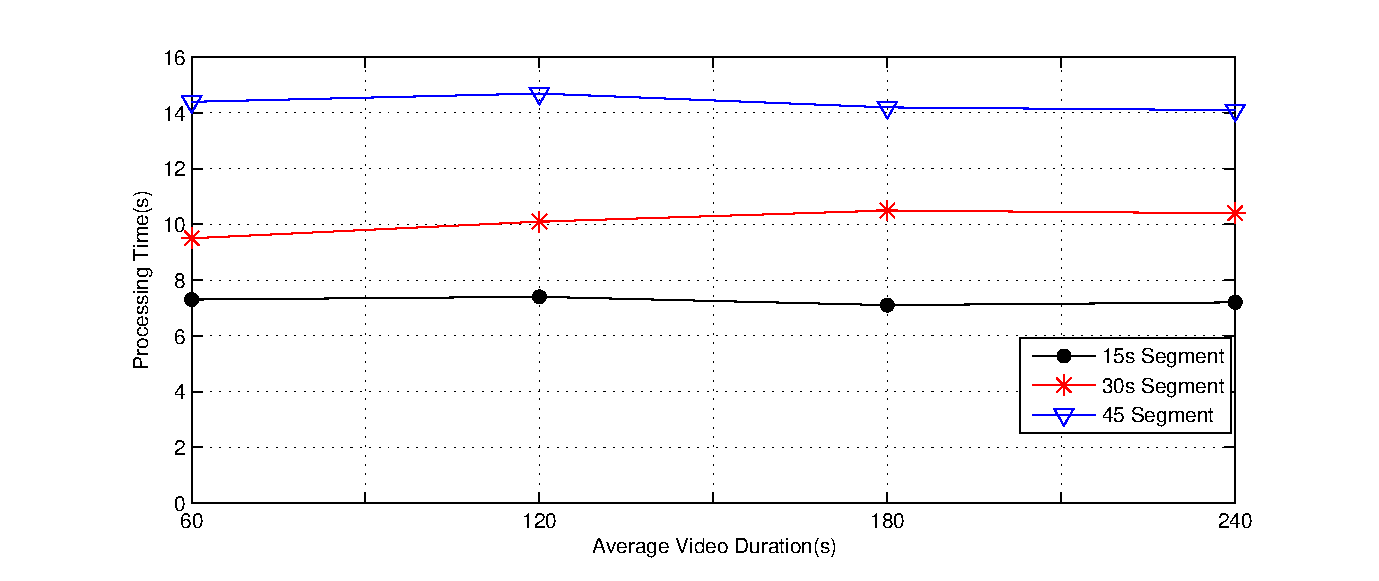
\epsfig{file=pics/videosegment.eps, height=1.7in,width=3.4in}
% %\vspace{-1mm}
% \caption{Average Video Segmentaion Time For different Duration}
% \vspace{-6mm}
% \label{fig:video}
% \end{figure}

% \textbf{Image Resize Tradeoff}
% \begin{figure*}[!t]
% \centering {
%     \subfigure[Average CEDD Execution Time Per Image for different SIZE ]{\includegraphics[width=1.6in]{pics/cedd.eps}\label{fig:resize_1}}
%     \hfil
%     \subfigure[Average Time of Resizing image to Different SIZE]{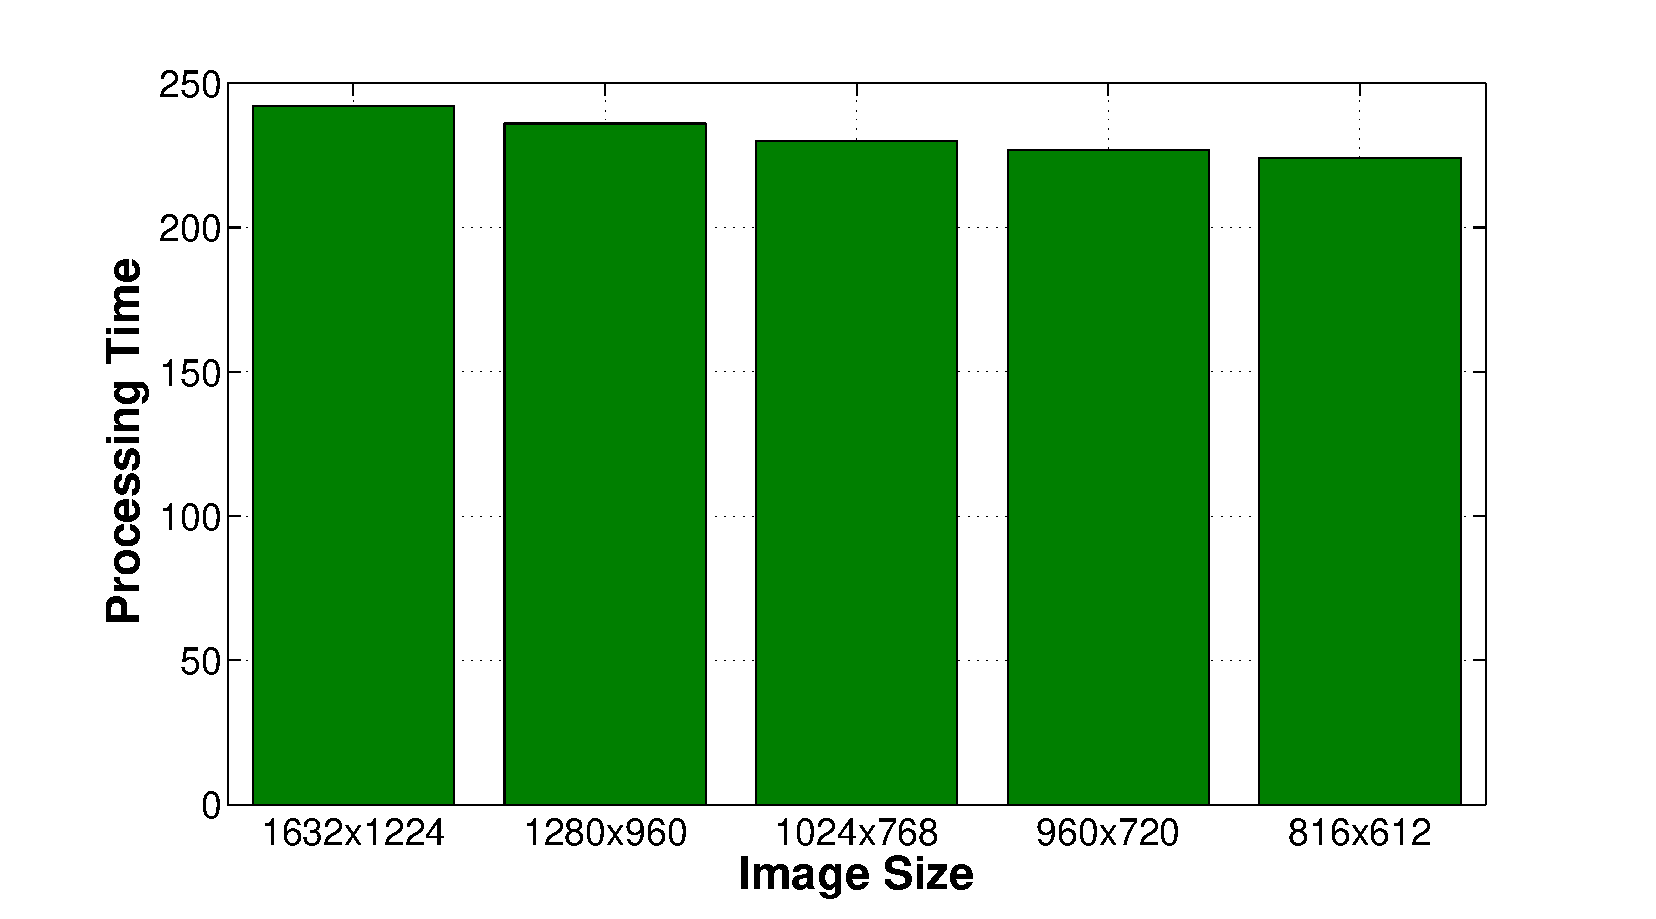
\includegraphics[width=1.6in]{pics/resizing.eps}\label{fig:resize_2}}
%     \hfil
%     \subfigure[Average Error Rate of KMeans Clustering for different Size]{\includegraphics[width=1.6in]{pics/kmeans.eps}\label{fig:resize_3}}
%     \hfil
%     \subfigure[Average Error Rate of Top K for different Size]{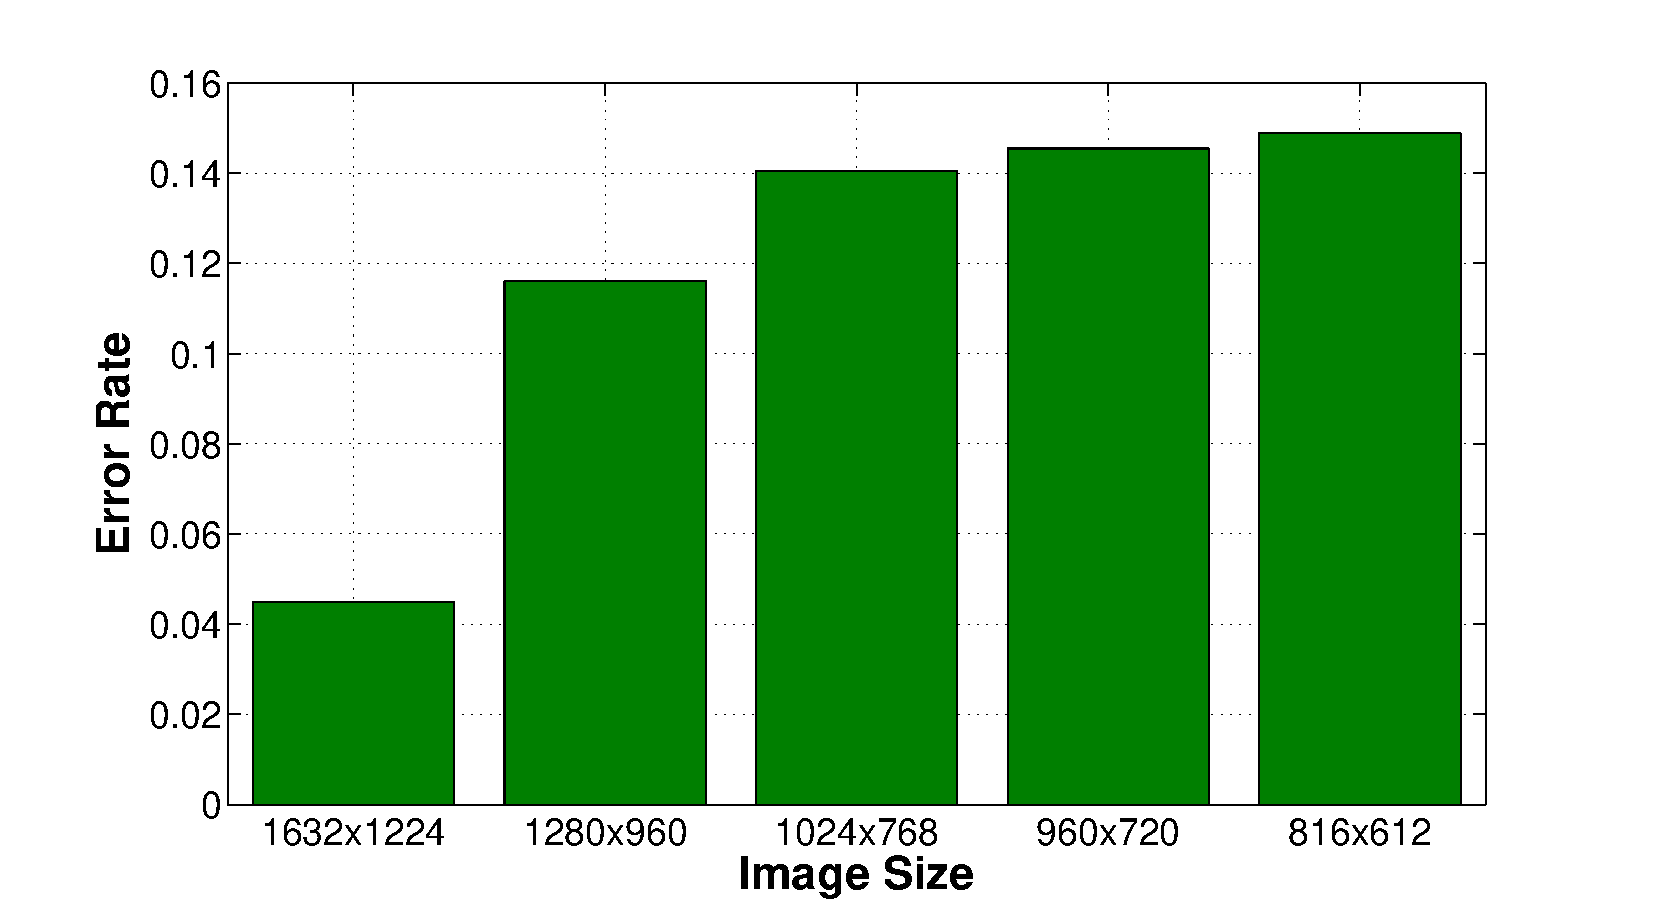
\includegraphics[width=1.6in]{pics/topk.eps}\label{fig:resize_4}}
% }
% \vspace{-1mm}
% \caption{Average Video Frame Extraction Time For Different Duration and Frequency}
% \vspace{-6mm}
% \label{fig:resize}
% \end{figure*}

% From the results, we will find 1280x960 is a good balance point here for the tradeoff of accuracy and processing time.

%\vspace*{-0.75ex}
\subsubsection{Leveraging a Crowd-Sensing Framework}
\label{sec-3-2-4}

MediaScope leverages an existing, publicly available, crowd sensing
programming framework called Medusa~\cite{Medusa}.
%
Medusa provides high-level abstractions for specifying the steps
required to complete a crowd-sensing task: in our case, uploading the
feature vectors can be modeled as a crowd-sensing task and so can the
upload of selected media objects.
%
Medusa employs a distributed runtime system that coordinates the
execution of these tasks between mobile devices and a cloud service.
%
In MediaScope, MSCloud uses Medusa to distribute tasks and collect the
results; MSMobile consists of extensions to Medusa's runtime to
implement the Feature Extractor and the Object Uploader.
%

However, in order to support MediaScope, we needed to extend the
Medusa model, which was focused on tasks generated by human users.
%
We also needed to make several performance modifications in Medusa.
%
In the former category, we modified Medusa's programming language to
selectively disable Medusa's recruitment feature and data privacy
opt-in: these features require human interaction, and
MediaScope assumes that participants have been recruited and have
signed a privacy policy out-of-band.
%
We also added a data delivery notification system that
would allow Medusa's cloud runtime to deliver notification of data
upload to external servers, such as MSCloudDB.
%
In the second category, we modified Medusa's mobile device
notification system, which originally used SMSs, to use Google's C2DM
notification service, which greatly reduced the latency of task
initiation on mobile devices.
%
We also optimized several polling loops in Medusa to be
interrupt-driven, so that we could hand-off data quickly to components
within Medusa's runtime as well as to external servers.

% to implement \mscope on Medusa, we
% need to do following modifications.
% %
% Firstly, we need to reduce the latency in Medusa system.
% %
% Medusa originally using polling-based notification indicating stage
% completed, which polls database periodically (10s) to check whether a
% stage has finished.
% %
% We add the option of directly notify Medusa server to reduce latency.
% %
% In addition, Medusa server use short message to notify smartphones to
% distribute task, we found short message delivering introduces instable
% latency, sometime over X seconds, which is not suitable for our
% timeliness query case.
% %
% To tackle this, we implement a new push notification method through
% C2DM \ref{C2DM} to reduce the notification delay.
% %
% Secondly, we can now configure a Medusa task to nitify any external
% server for particular events, for example, in a uploading task, once
% there is a new file got uploaded, Medusa can notify any specified
% external server.
% %
% Thirdly, we make Medusa server accept machine-generated tasks for
% automatic distribute tasks.
% %
% Lastly, we make the transfer component of Medusa more flexible,
% supporting different uploading schemes instead of FCFS only and the
% uploading scheme can be changed from Medusa server.
% %

% \textbf{\mscope on Medusa:} with aforementioned modification to Medusa, we can implement \mscope completely on top of it. MSCloud will periodically generate feature extraction and uploading task, which will ask all the smartphones to extract the feature of their newly captured image objects (by providing the last object id on each phone). Uploaded file containing extracted features will firstly be uploaded to Medusa server, Medusa notify MSCloud and then MSCloud parse the file and store the features in the MSCloudDB. Whenever there is a query, MSCloudQ will generate the uploading task to all the smartphones, associated with each phone's selected media objects, assigned credits and timeliness bound for the query. Then MSMobile will start to upload selected media objects based on current uploading scheme (for default OPTNAME). Once a file got uploaded to Medusa server, a notification will be sent to MSCloud, MSCloud collect such file and get prepared to return the query result page.

%\vspace*{-1ex}
\section{Evaluation}
\label{sec-4}

% \subsection{Methodology}
% \label{sec-4-1}

In this section, we evaluate the performance of MediaScope.
%
Although MediaScope's credit assignment algorithm is optimal in a
pseudo-polynomial sense, we are interested in its practical
performance under bandwidth variability.
%
Furthermore, in practice, since query arrival cannot be predicted
ahead of time, the practical performance of MediaScope may deviate
from the optimal.
%
Finally, it is instructive to examine alternative scheduling
mechanisms to quantify the performance benefits of MediaScope's
algorithms.
%
We are also interested in the overhead imposed by MediaScope; since
timeliness is an essential attribute of many queries, system
inefficiencies can impact query completeness.

All our experiments are conducted on a prototype of MediaScope.
%
MSCloud is written mainly in Python; PHP and Python are used for
MSCloudQ web interface.
%
The implementation of MSCloud is about 4300 lines of PHP and Python
code, and MSMobile requires about 1150 lines of C and Java code
(measured using SLOCCount~\cite{sloccount}).
%
% Overall 4093 lines of Python code, and about 200 lines of PHP on
% MSCloud, added/modified 931 lines of java code and 223 lines of C code
% to Medusa on MSMobile side (Counted by SLOCCount).
%

Our experiments use commodity hardware, both for MSCloud and the
mobile device.
%
We use up to 8 Android phones, which are either the Galaxy Nexus or
the Galaxy SIII.
%
MSCloud runs on a Dell XPS 7100 (six-core AMD Phenom II X6 1055T 2.8
GHz processor and 6MB built-in cache).

\begin{figure*}
\centering
\begin{minipage}[t]{5.8cm}
\centering
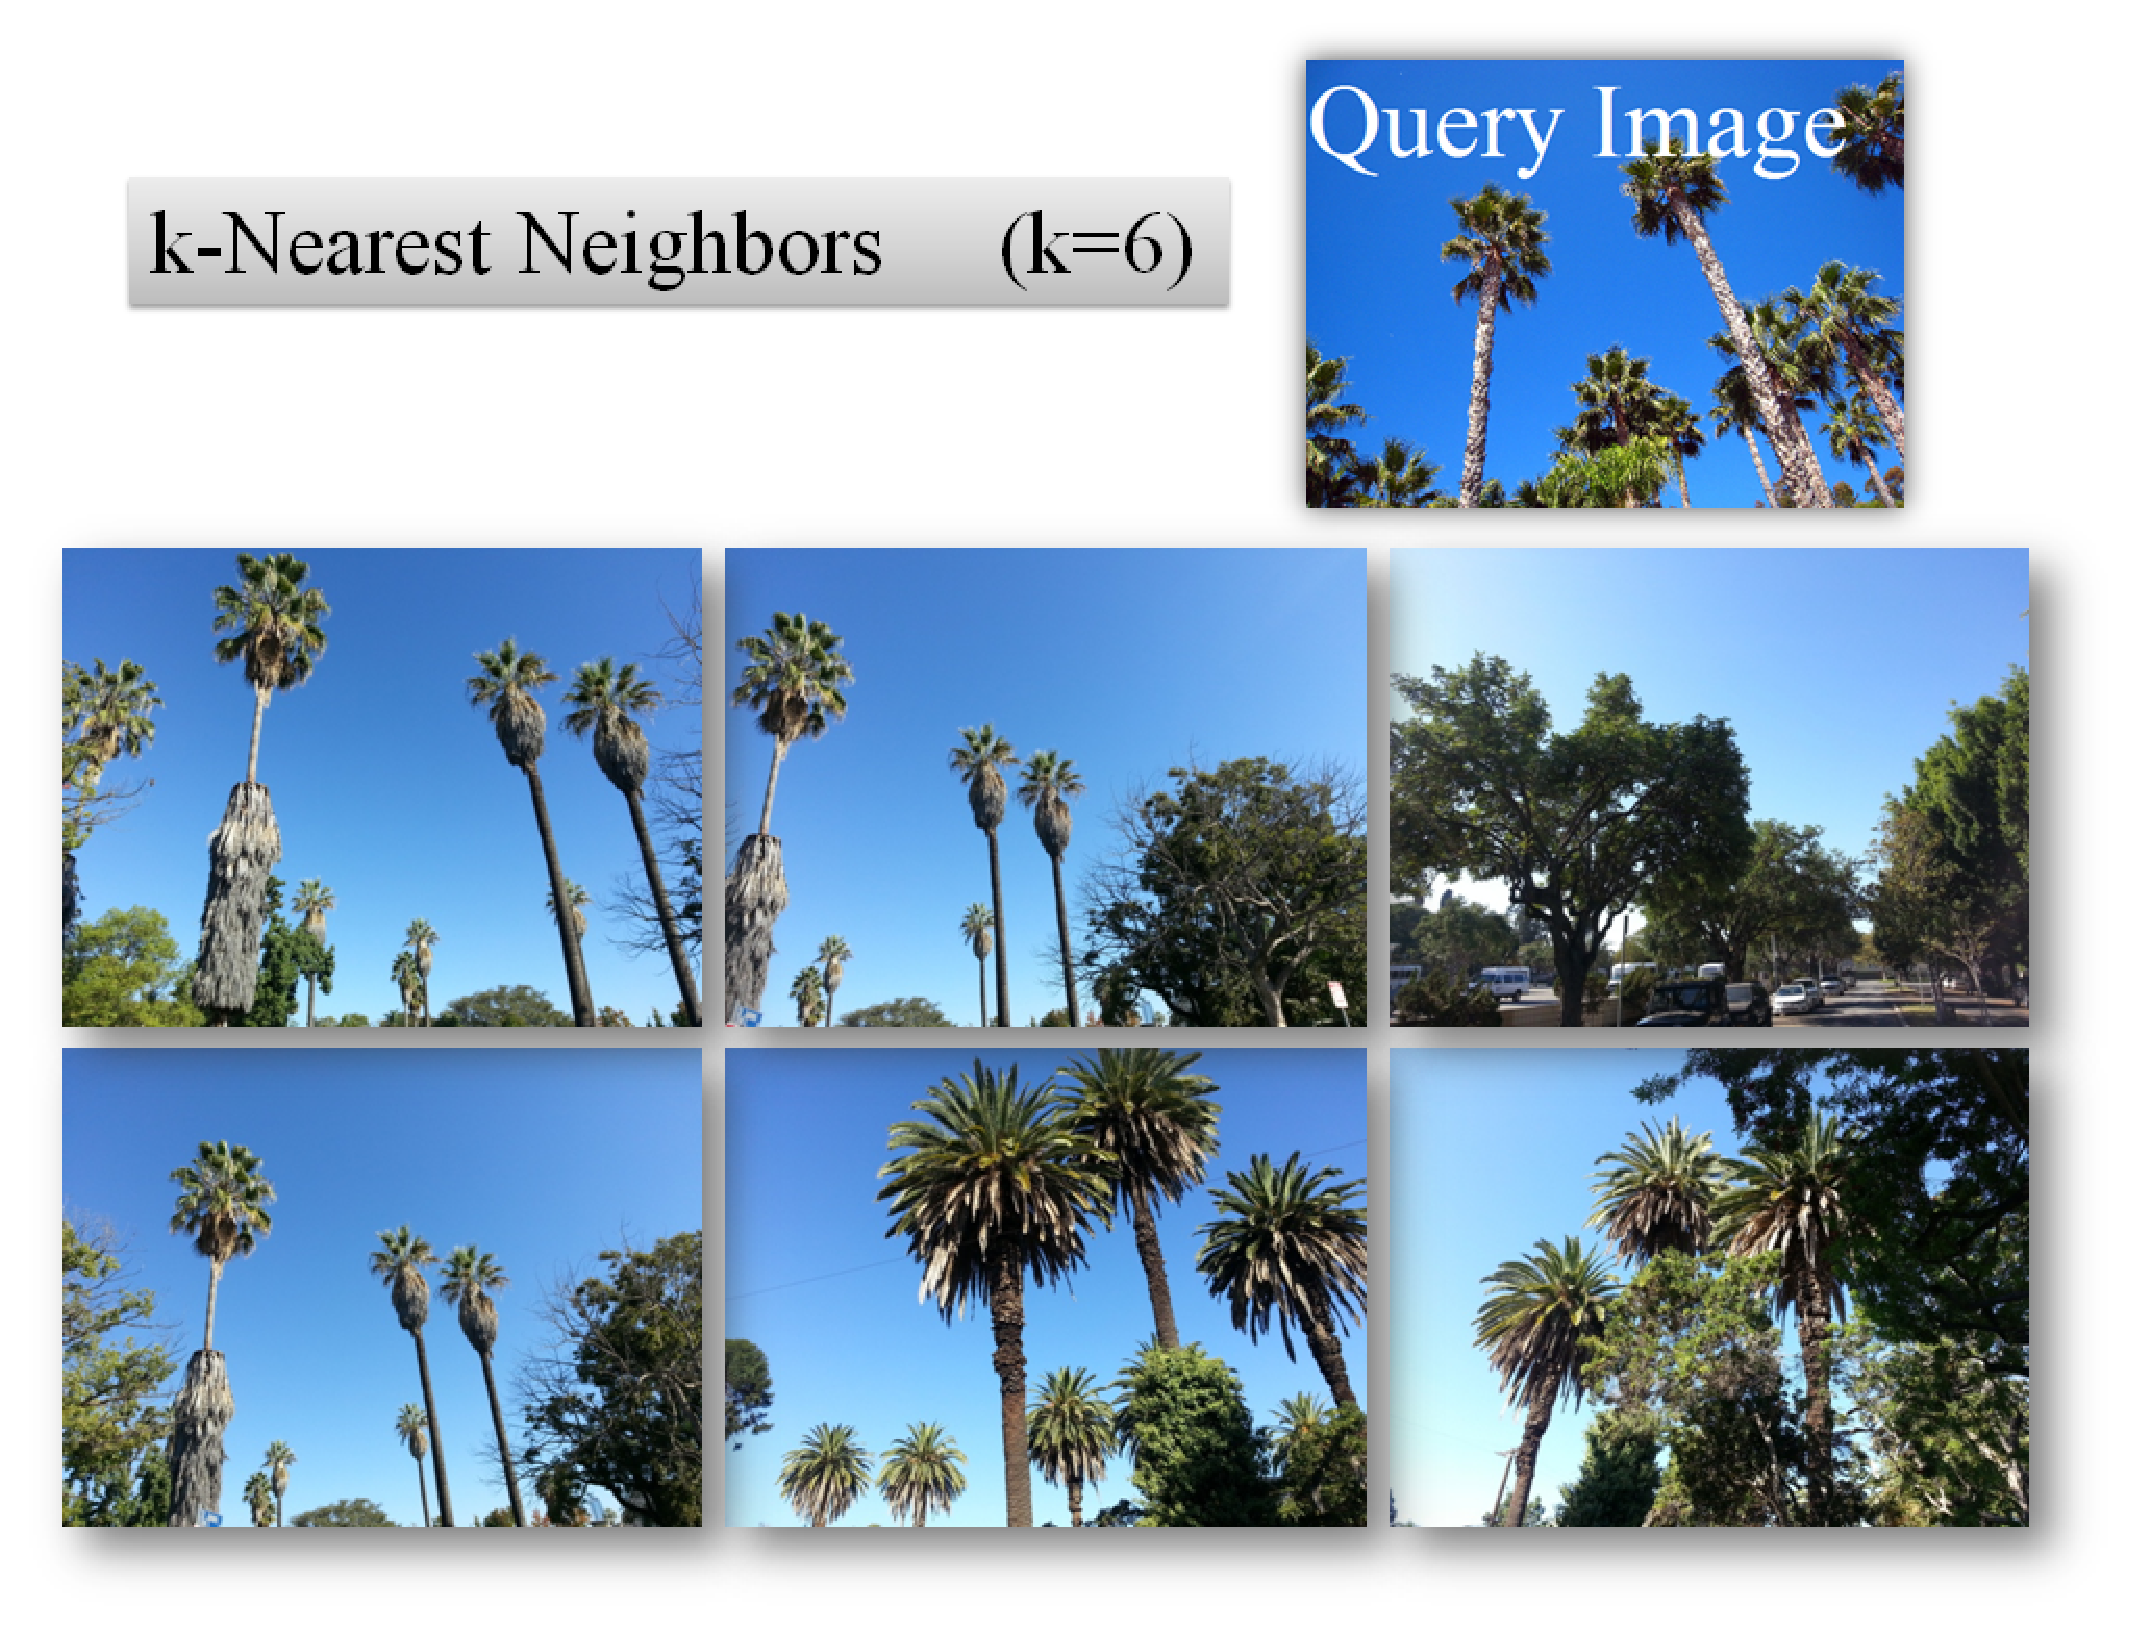
\includegraphics[width = 5.6cm]{pics/1.eps}
\centering \caption{K Nearest Neighbor Result} \label{fig:top_k}
\end{minipage}
\begin{minipage}[t]{5.8cm}
\centering
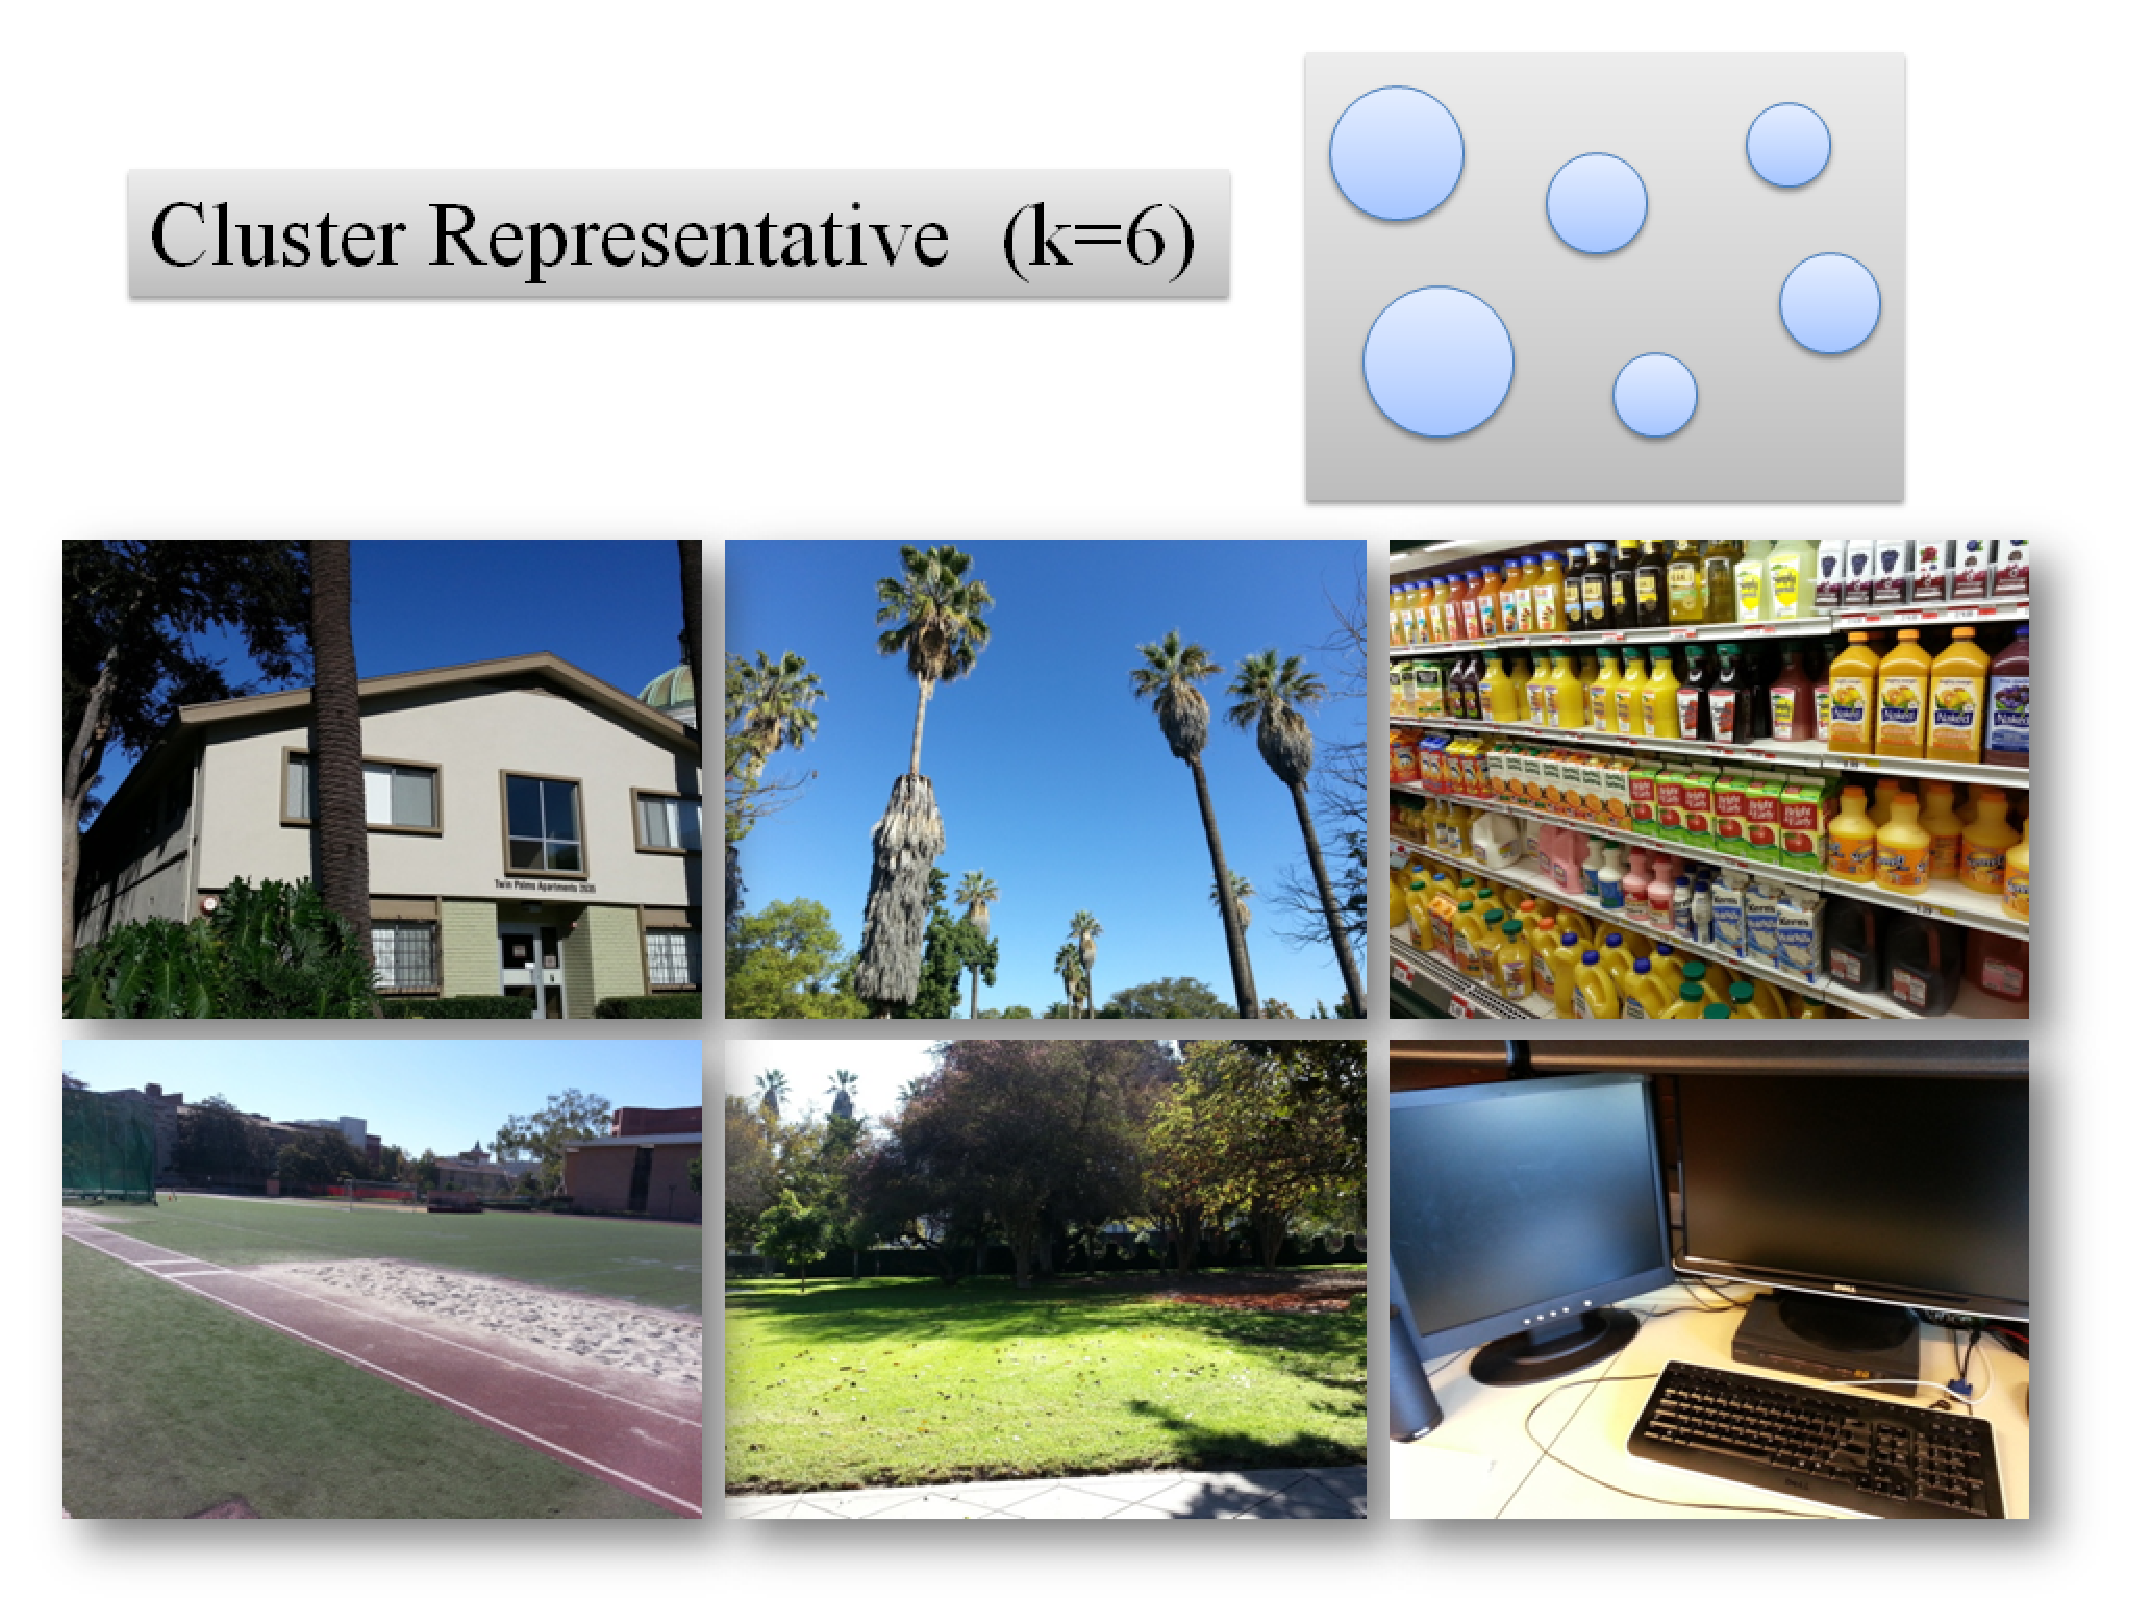
\includegraphics[width = 5.6cm]{pics/2.eps}
\centering \caption{Cluster Representative} \label{fig:cluster_representative}
\end{minipage}
\begin{minipage}[t]{5.8cm}
\centering
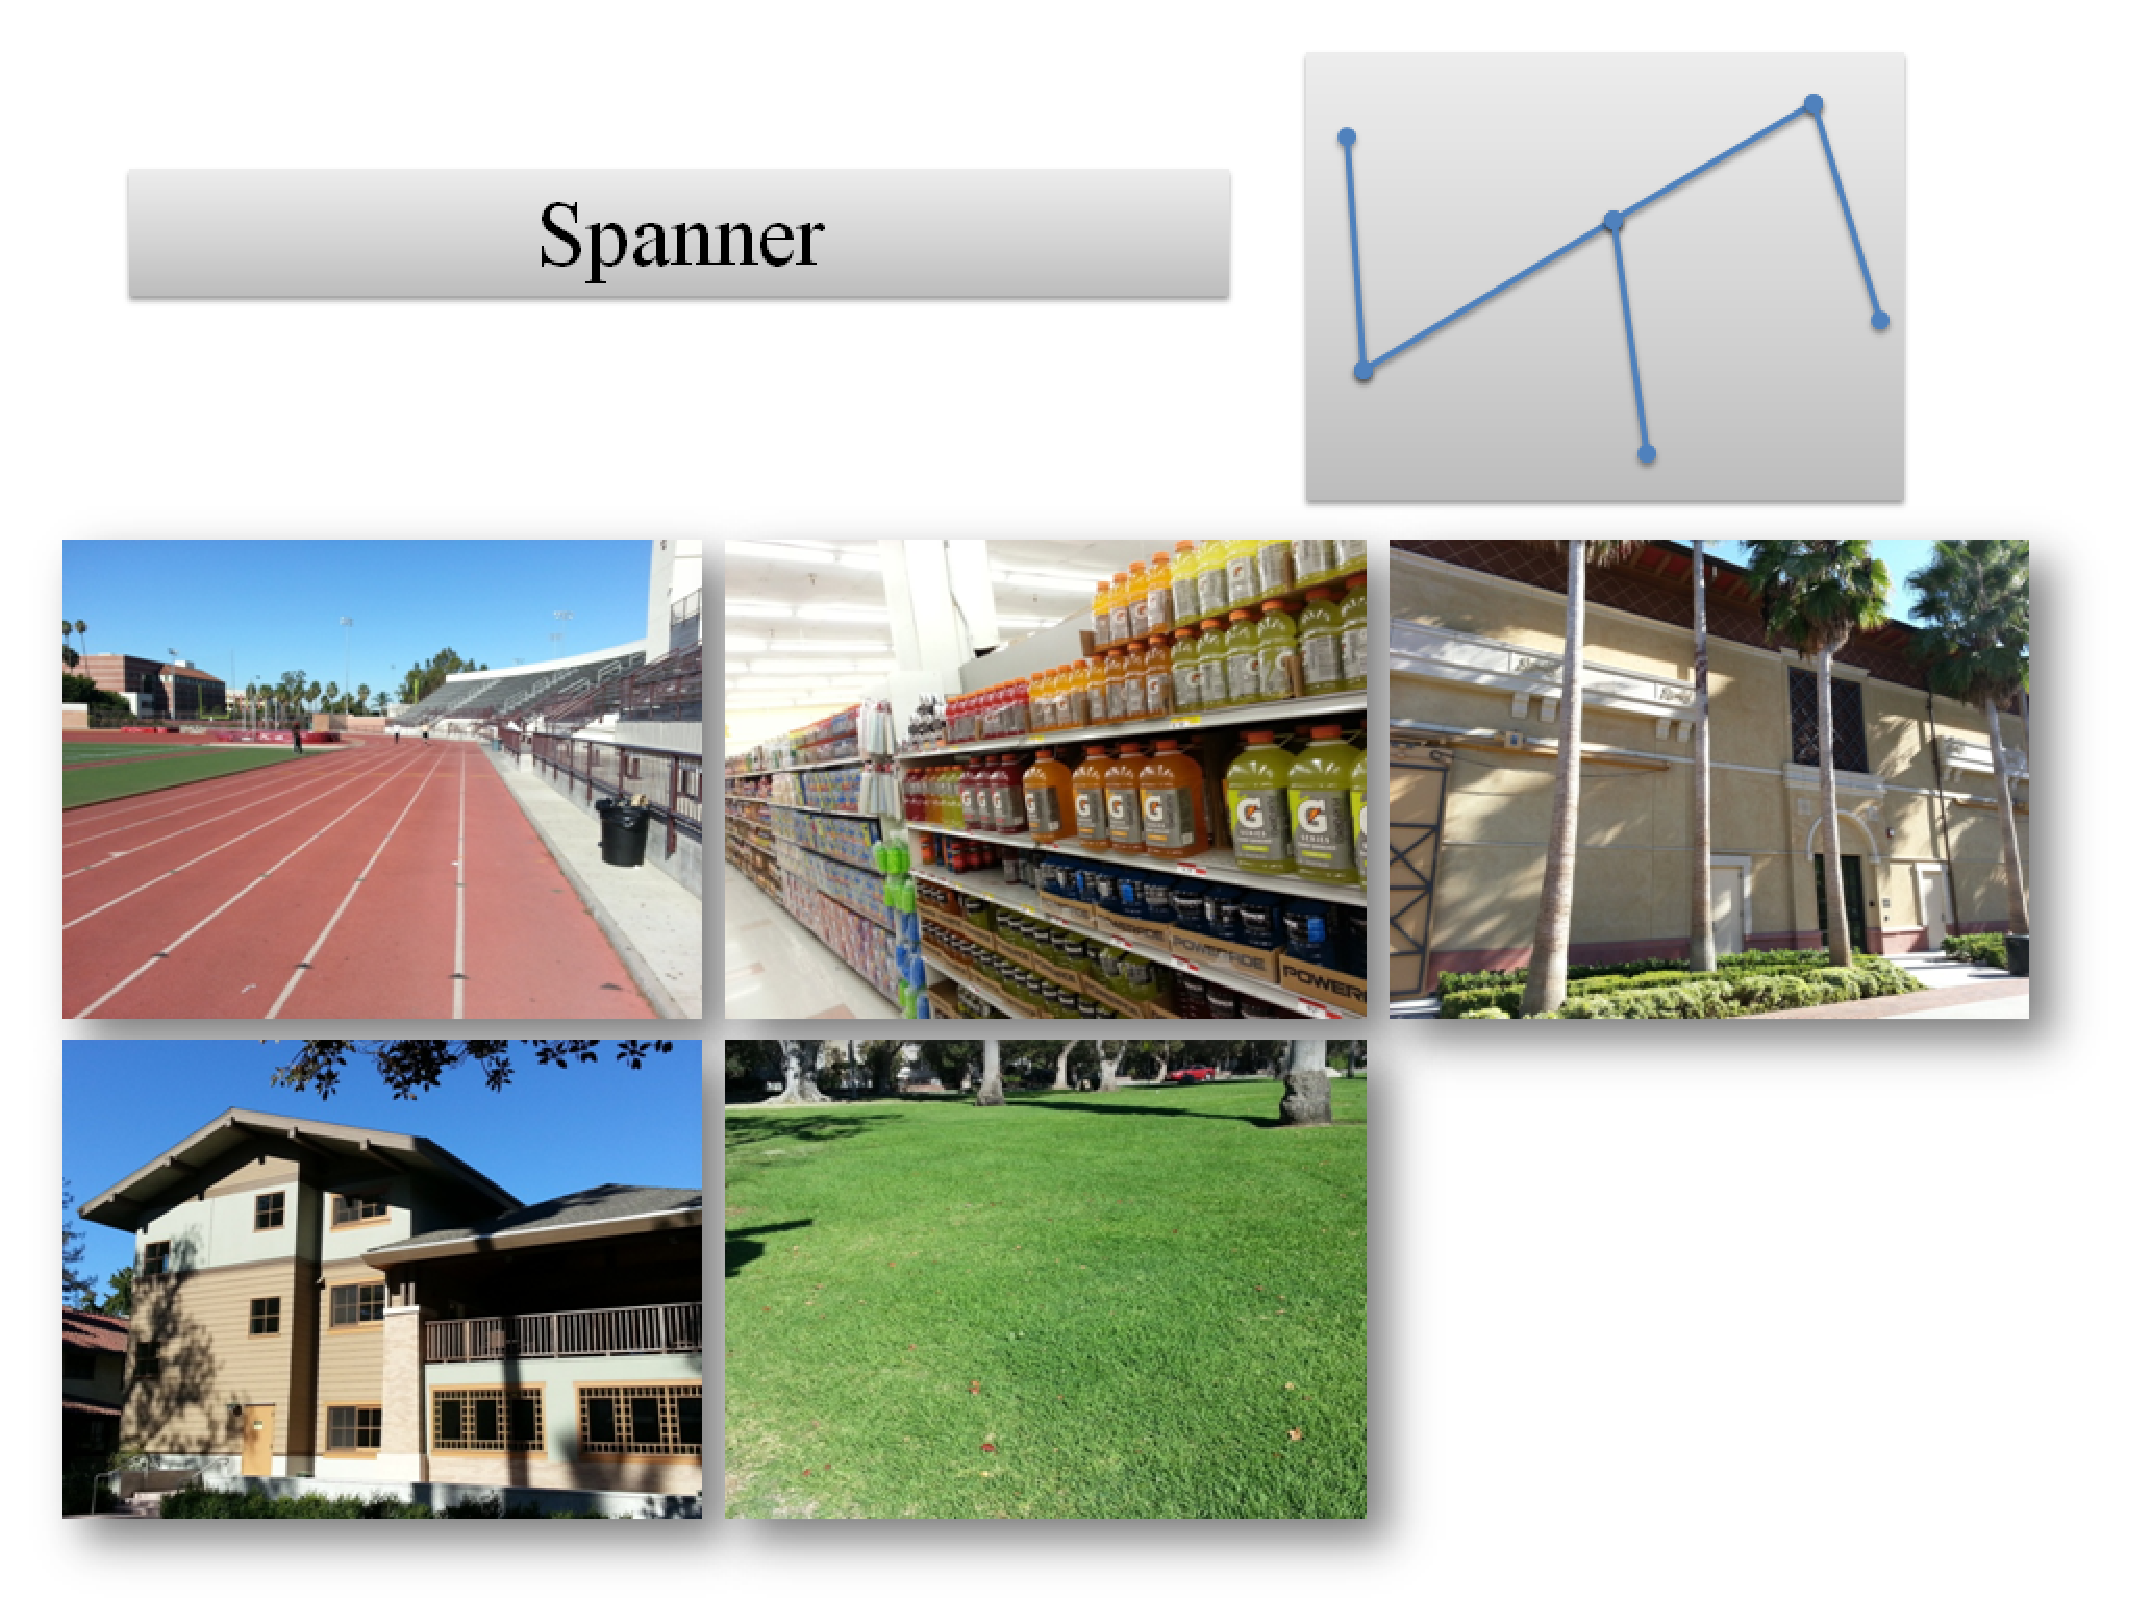
\includegraphics[width = 5.6cm]{pics/3.eps}
\centering \caption{Spanner} \label{fig:spanner}
\end{minipage}
\end{figure*}

Before describing our results, we give the reader some visual
intuition for the usefulness of MediaScope.
%
Figures~\ref{fig:top_k}, ~\ref{fig:cluster_representative},
and~\ref{fig:spanner} show the results of three different queries: a K
nearest neighbor query, a Cluster Representatives query and a Spanner
on a set of six groups of photos: a university campus, a garden, a
view of the sky framed by trees, an athletics track, a supermarket,
and a laboratory.
%
Notice that the cluster representatives query identifies
representatives from each of groups, while the Spanner extracts
qualitatively different pictures, while the K nearest neighbor query
extracts matching images as we might expect.
%
%In contrast,... \ramesh{Will fix after top-K}

% We run our $K Cluster Representative$ query and $Spanner$ query on the photo set with  total 175 feature vectors (some from short videos), and results are shown on Figure~\ref{fig:sample}
%  }

%\vspace*{-0.75ex}
\subsection{Query Completeness}
\label{sec-4-2}

In this section, we evaluate query completeness in the presence of
concurrent queries.

\mypar{Metrics and Methodology.}
%
Our metric for query completeness is the total credit associated with
all the query results successfully uploaded before their timeliness
bounds.
%
We evaluate several \emph{query mixes} (described below), with
different concurrent queries of query types that arrive at different
times and have different timeliness bounds.
%
These queries are all posed on 320 images captured on 8
mobile devices.
%

Our experiments are conducted as follows.
%
For each query mix, we first compute the results of each query and the
credit assigned to each result object.
%
This computation yields a \emph{trace}, on each mobile device, of
objects, their associated credits and the arrival time.
%
We use this trace to replay the credit-based scheduling algorithm
during repeated runs and report the average of 10 runs.

This trace-based methodology is also useful in comparing MediaScope's
credit-based scheduling algorithm (henceforth, \emph{MSC}) with
several alternatives.
%
For each alternative, we replay the trace for that particular
scheduling algorithm.
%
We consider the following alternatives: an \emph{Omniscient} algorithm
that knows about future query arrivals; a \emph{Max Credit First
  (MCF)} that always selects the object with a maximum credit to
upload; a \emph{Round Robin (RR)} that allocates bandwidth fairly to
each concurrent query so that, in each round, the object with the
highest credit from each query is uploaded; and an \emph{Earliest
  Deadline First (EDF)} scheduler that always schedules that object
with the earliest timeliness bound first, breaking ties by credit.
%
The Omniscient algorithm demonstrates the benefits of lookahead, while
each of the other algorithms has at most one of MSC's features
(timeliness-, credit-, and bandwidth-awareness).

In our experiments,  each mobile device contains a number of images
taken with its camera.
%
These images are naturally of different sizes because they have
different levels of compressibility.
%
Furthermore, we make no attempt to control network variability; upload
bandwidths in our experiments vary and MSC estimates upload bandwidth
by measuring the average speed of the last upload (MSC's algorithm
needs uses this estimate for $t(o)$).

%
% In our evaluation, 8 Android phones each has captured roughly 40 images in advance for querying. We design several series of concurrent queries, including all the query types we implemented. For each series of concurrent queries, we record the starting time and deadline of each query, as well as selected objects with its credits for repeating the process of uploading for $10$ times. For each generated series of concurrent queries $\mathbb{Q}$, total credit received $c(\mathbb{Q})$ will be considered as the (only? fairness?) matric.

% We will compare our scheme described in \ref{sec-3-2-2} against a variety of alternative approaches, namely \textit{Max Credit First}, \textit{Earliest Deadline First} and \textit{Round Robin}. Max Credit First (MCF) scheme always picks the one with the maximum credit to upload; Earliest Deadline First (EDF) scheme uploads the object with the earliest deadline; \textit{Round Robin} allocates bandwidth fairly to all the ongoing queries, in each round, every query will be uploaded one media object. The last competitor acts as a theoretical upper bound, which knows all the future queries $\mathbb{Q}$ at time $0$ and uploads based on the optimal schedule, we call it $\textit{Optimal with Full Knowledge} (FULL)$.

\begin{figure*}[t]
  \begin{minipage}{0.32\linewidth}
    \centering \epsfig{file=pics/different_queries.eps, width=0.95\linewidth}
    % \vspace{-1mm}
    \caption{Different Query Mixes by Size}
    %\vspace{-6mm}
    \label{fig:different_queries}
  \end{minipage}
  \begin{minipage}{0.32\linewidth}
    \centering \epsfig{file=pics/different_times.eps, width=0.95\linewidth}
    % \vspace{-1mm}
    \caption{Different Query Mixes by Timeliness Bound}
    %\vspace{-6mm}
    \label{fig:different_times}
  \end{minipage}
  \begin{minipage}{0.32\linewidth}
    \centering 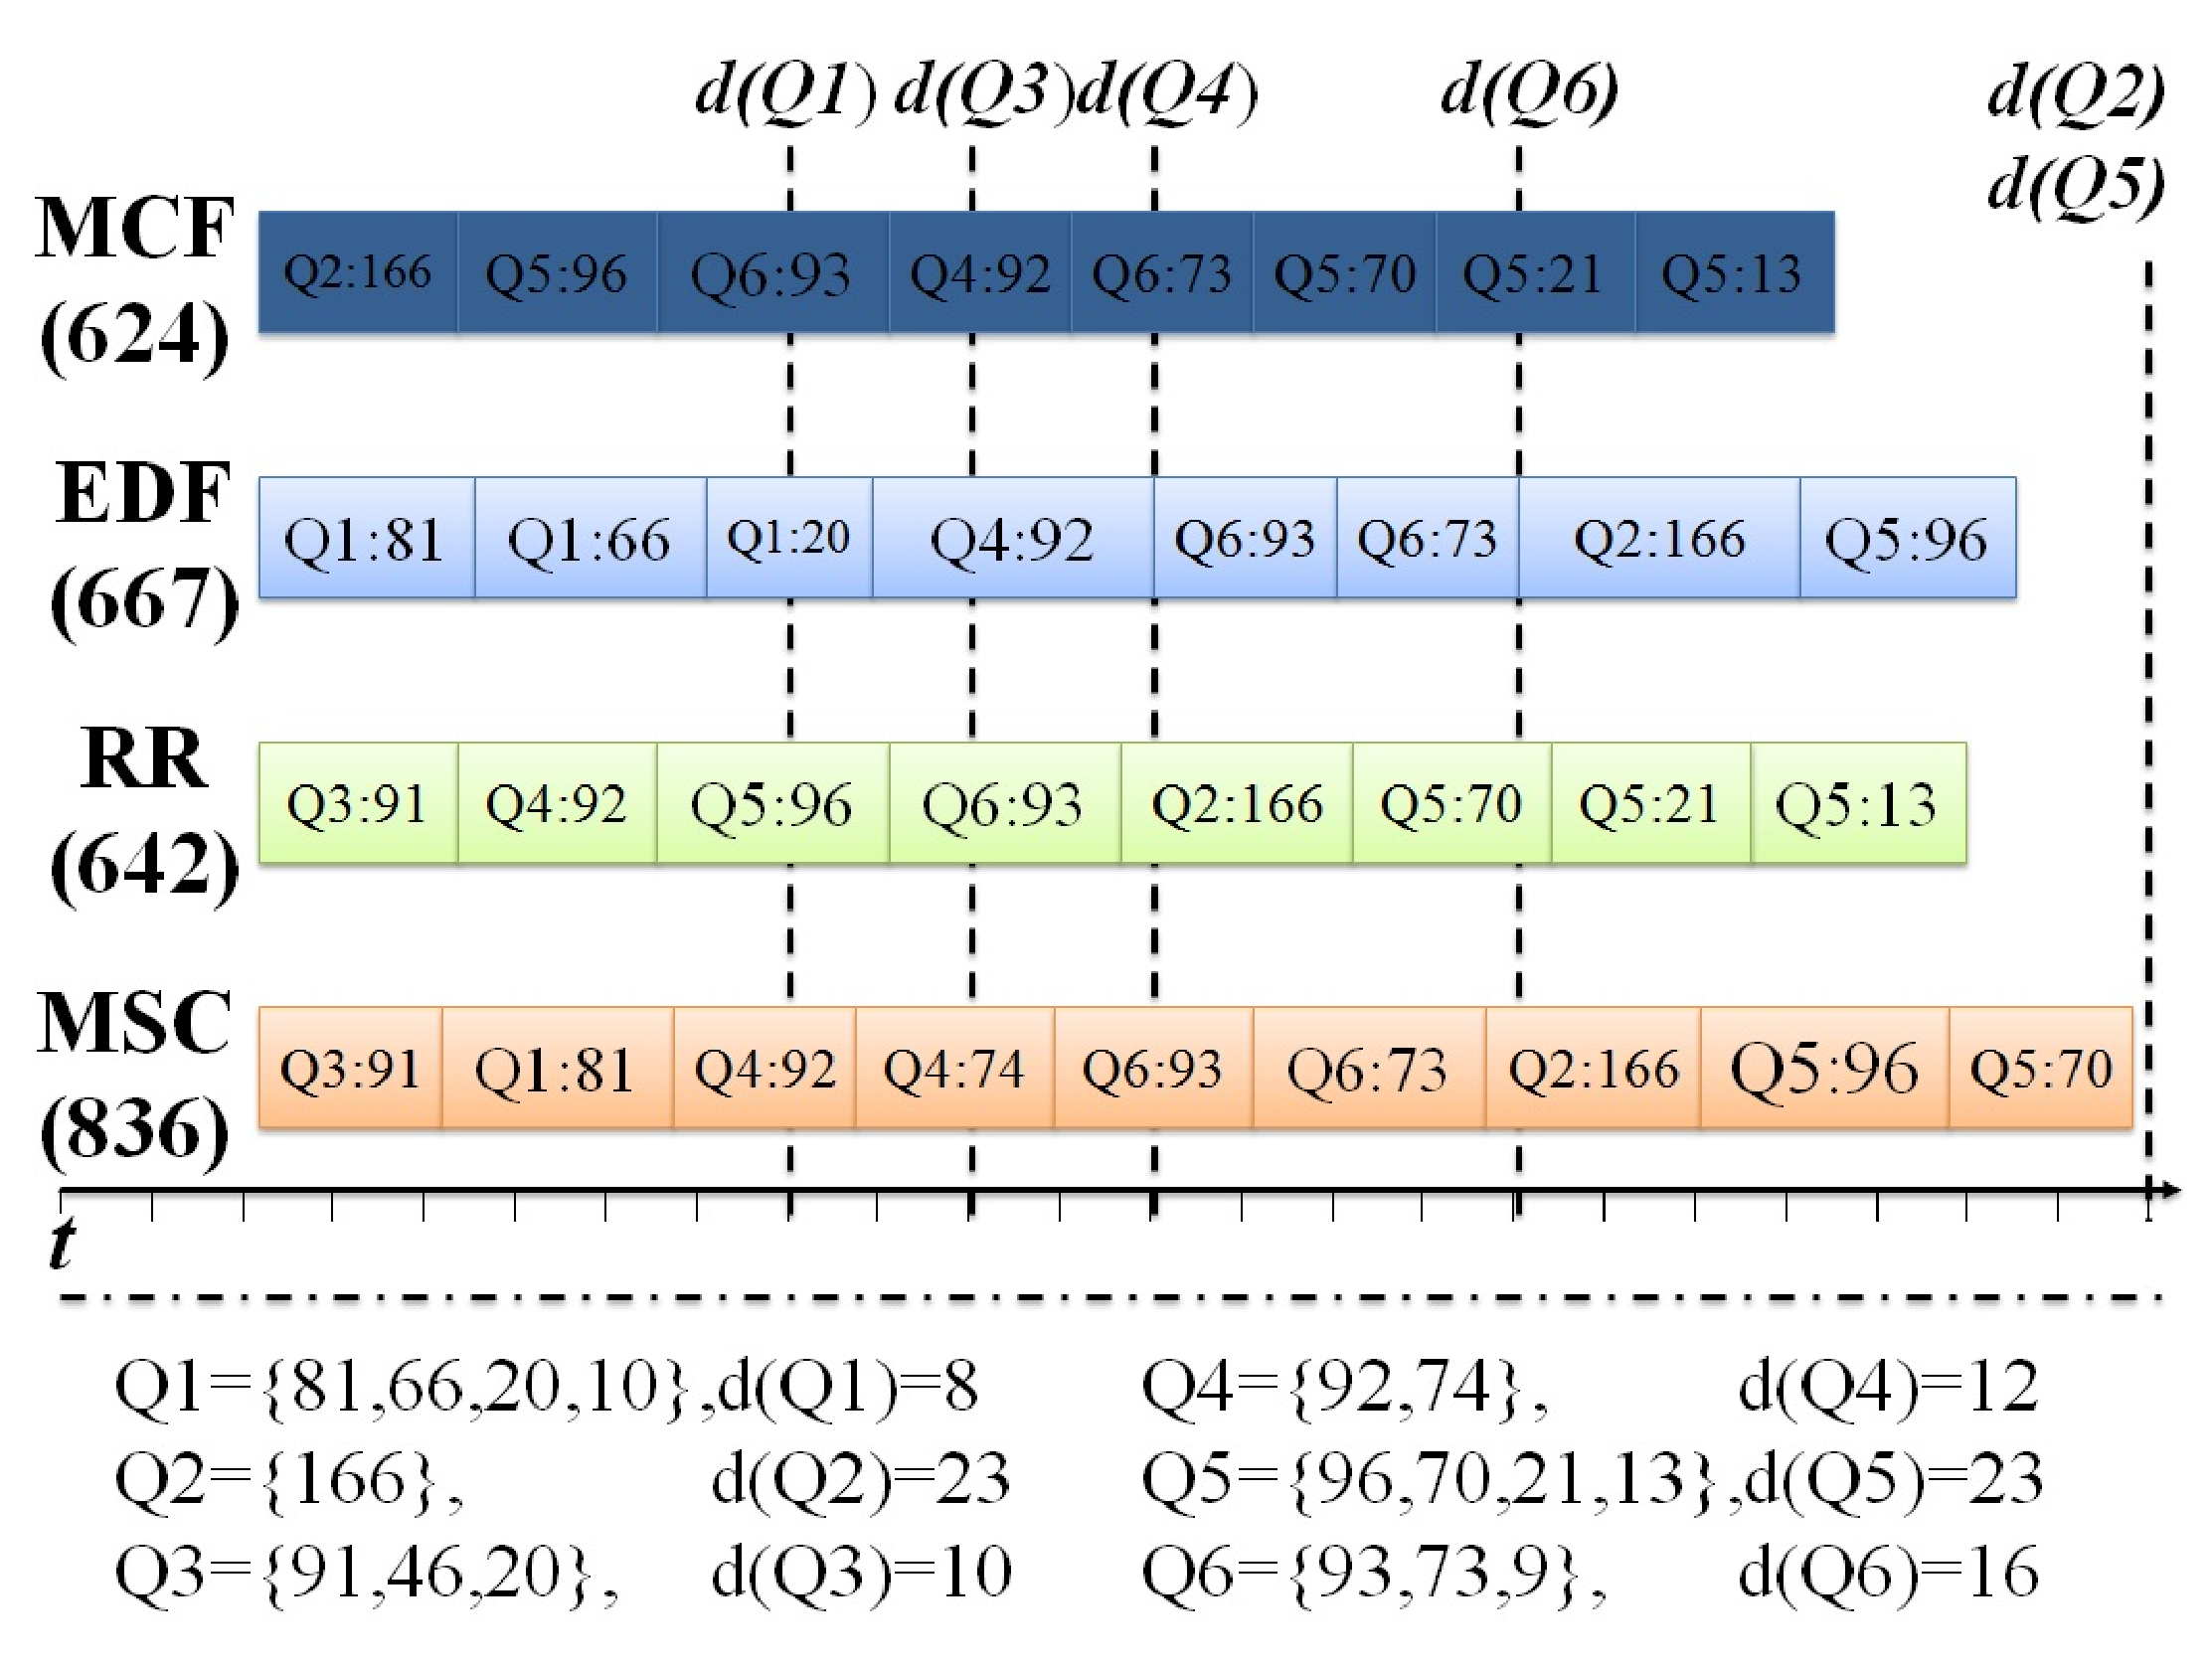
\epsfig{file=pics/timeline.eps, width=1.05\linewidth}
    %\vspace{-6mm}
    \caption{Sample Schedule Timeline}
    %\vspace{-6mm}
    \label{fig:timeline}
  \end{minipage}
\end{figure*}

\mypar{Results.}
%
Our first experiment compares the performance of these alternatives
for three different query mixes with different types of queries.
%
The first mix contains 4 queries, namely, 1 Top-K, 1 Spanner, 1
Cluster Representative and 1 Common Interest.
%
All the queries arrive at the same time but with different timeliness
bounds; thus, in this experiment there are no future arrivals and we
do not evaluate the Omniscient algorithm.
%
The second mix adds one more Cluster Representative query to the first
one, and the third is generated by adding one more Common Interest
query.
%
In each query mix, each query is assigned the same total credit.
% the total query completeness score for a given query mix can be
% obtained by multiplying the number of queries in the mix by 1000.

% All the query assign selected objects with credits up to 1000.
% %
% So in this setting the maximal credits we can get is the query number
% times 1000.
% %

Figure~\ref{fig:different_queries} shows the performance of various
schemes.
%
MSC achieves at least 75\% completeness across all three query mixes,
and its performance improves by 5\% as the number of queries increases
from 4 to 6.
%
Although a 75\% completeness rate seems pessimistic, we remind that
reader than MSC is optimal, \emph{so no other scheduling scheme could
  have done better than this}; in other words, for this query mix,
this is the best result that could have been achieved.

Furthermore, MSC outperforms other schemes significantly.
%
The superior performance of MSC comes from its
timeliness-awareness, credit-awareness, and adaptivity to available
bandwidth.
%
By contrast, approaches that lack one or more of the features have
much lower completeness rates.
%
Thus, EDF does not take into account an object's credit, and thus
might waste bandwidth on objects with an early deadline but small
credit; on average, EDF achieves 55\% completeness.
% \ramesh{Fix.}\xing{percentage added}
%
RR is unaware of timeliness constraints, but uploads the result
objects for each query in a round-robin fashion.
%
It is comparable in performance to EDF, achieving 52\% completeness on
average. % \ramesh{Fix}\xing{percentage added}
%
RR's poor performance arises from two factors: first, because it
ignores timeliness constraints, it uses transmission opportunities by
sometimes transmitting objects which could have been deferred without
violating data timeliness bounds; second, RR gives equal transmission
opportunities to queries, even though, on a given mobile device, one
query may contain objects with far more credit than another query.
%
MCF improves upon RR in the second aspect, in that it always transmits
the object with the highest credit first; in so doing, it achieves an
average completion rate of 59\% and is significantly better than EDF
and RR. % \ramesh{Fix}. \xing{percentage added}
%
However, MCF is still noticeably worse than MSC, primarily because MCF
ignores timeliness constraints and sometimes transmits objects that
could have been deferred without violating timeliness bounds.

% The reason is, RR achieves fairness on each phone, but not globally.
% %
% Consider the extreme case where $Q_1$ assigns several important
% objects to $P_1$, on the other hand $Q_2$ and $Q_3$ assign not
% important objects to phone 1, it is obvious that $P_1$'s local
% fairness is not efficient since in this case $Q_1$ should get more
% resources.
% %
% The result of MCF is not bad, since it greedily earn max credit in
% every round.
% %
% MCF is an effective scheme but anyway it has not consider deadline so
% in the worst case, MCF can perform as bad as only $50\%$ of optimal
% scheme.
% %
% Our scheme performs the best in all the settings, uploaded roughly
% $75\%$ of the total credits.
% %
% In addition, as the number of concurrent queries increasing, our
% scheme performs better compared to other competitors.
% %
% The reason can be explained by the value of ``planning'': when there
% is lacking the opportunity of planning, simply MCF would be an
% effective solution (consider two extreme cases, when there is no
% concurrency and there are bursty queries); however when there are
% modest concurrent queries, our scheme can leverage the advantage of
% planning.
%

In order to get more insight into the relative performance of these
schemes, we consider variants of the 6-query mix which have different
combinations of arrival rates and deadlines.
%
Figure~\ref{fig:different_times} plots the results of these experiments.

In the first query mix, three of the six queries arrive first with the
timeliness bound of 20 seconds.
%
The remaining three queries arrive within three seconds, but have a
relatively tight timeliness bound of 6 seconds.
%
In this sense, they \emph{interrupt} the first set of queries.
%
This query mix is designed to demonstrate the benefits of
timeliness-awareness.
%
In this somewhat adversarial setting, MSC still outperforms other
schemes but has a much lower completeness rate of about
60\%. % \ramesh{Add.} \xing{percentage added}
%
RR performs poorly, but EDF performs comparably to MCF; this is not
surprising because EDF is timeliness-aware.
%
Even so, EDF does not perform as well as MSC because it ignores credit
values and uploads objects with lower credits unnecessarily.

% Fig. \ref{fig:different_times} shows the same queries of above
% experiment of 6 queries, but this time we vary the arriving time and
% the deadline of such queries. The first setting which we call it
% ``interrupted'' setting, where 3 queries come first, with late
% deadline of 20 seconds, while another 3 queries come 3 seconds later
% but with relatively tight deadline of 6 seconds. The latter 3
% queries act as ``interruptor'', and this setting is evaluating which
% scheme can handle these interruptors well. MCF is always a strong
% scheme, however, we see EDF performs also good in this case because
% when the interruptor came in it, it stopped to upload interruptor's
% objects. Our scheme is still the best among all the schemes.

In the second query mix, 6 queries with the same timeliness
requirement arrive in a staggered fashion, with each query arriving
three seconds after the previous query.
%
This illustrates a setting where queries arrive frequently but the
arrivals are not synchronized.
%
In this setting, MSC achieves a completeness rate of nearly 80\%, and,
not surprisingly, MCF comes quite close with a completeness rate of
71\%.
%
Since all queries have identical timeliness bounds, it is not
surprising that a credit-aware scheme like MCF performs well.
%

The third query mix represents a complex pattern where queries arrive
at different times and have different deadlines.
%
For this mix, the performance advantages of MSC are clear, since this
mix requires a scheduling scheme to be both credit and
timeliness-aware.

% but all queries have the same timeliness bound.
% \xing{In the second query mix, 6 queries come one by one, 3 seconds after previous query, and of the same timeliness bound of 6 seconds.}
% %
%  \xing{In a setting that there would be frequent future queries coming in,} This mix is designed to illustrate the importance of credit awareness,
% and one might expect that, in this setting, MCF would perform best.
% %
% Indeed, we find that MCF achieves a completion rate of about 71\% on
% average. \ramesh{Fix.} \xing{percentage added}
% %
% In this setting, MSC is comparable to MCF; by design, it uploads the
% highest credit objects for the first set of queries, and then adapts
% its uploading schedule when the second set of queries arrives.

% Surprisingly, EDF also performs well in this setting...
% \ramesh{Will re-write this once the new experiments are in}

% The second setting sets all the queries with the same deadlines, similar to interrupted setting, three queries come 3 seconds later. It is clear that if all the queries are of the same deadline, then MCF would be the optimal solution. However, our scheme might be dangerous in this setting, because our scheme tries to plan the uploading but incoming queries might ``disagree'' the original plan and make our scheme ``regret'' about previous decision. But from the result we can see our scheme performs as good as the optimal one, MCF. The reason is, our scheme not only do the theoretical optimal schedule, but also switch the selected one with the maximum credits but of the same deadline. With this simple modification, our scheme would hardly ``regret'' about this decision when the future queries come in.

% The third setting is the most complicated one and with the most value
% of planning, where queries' arriving time are different as well as deadlines. In this
% setting, MCF, EDF and RR all are not comparable to our scheme.
% \ramesh{Will rewrite this when the new results are in.}

Finally, for all these query mixes (Figure \ref{fig:different_times}),
MSC is comparable to the Omniscient scheme, which knows the arrival
times of different queries.
%
Intuitively, because MSC continuously adapts its transmission
schedules when new queries arrive, it can make a different decision
from Omniscient only at the times when queries arrive.
%
To be more precise, say a new query arrives at time $t$: Omniscient
might have scheduled an upload of an object for the new query starting
at time $t$, but MSC has to wait until the object being uploaded at
$t$ finishes, before it updates its schedule.
%
This difference can be fixed by adding \emph{preemption} to the
scheduler, aborting the current transmission if it does not have the
highest priority; we have left this to future work.
% \ramesh{Xing,
%   please check.} \xing{generally correct. but in the extreme case, our scheme may `regret' about already uploaded ones: say, if I know there would be a bursty queries coming soon with higher credits than what I have, I don't need to do any 'schedule', or say any 'planning' is bad idea; except for MCF, MCF is good for bursty, by bursty I mean lots of incoming queries with higher credits...}

% it can at most be worse than
% Omniscient by the credit associated with one object (the one being
% transmitted

% we added the ``cheating scheme'', FULL, which know all the incoming
% queries at time 0. But in all three settings, we see our scheme's
% performances are pretty close to it, showing that optimal scheduling
% based on current queries is indeed a good intuition for the real case
% where new queries will join at any time, at least for the modest
% concurrent queries case.

To get some more insight into the differences between the scheduling
algorithms, Figure~\ref{fig:timeline} plots the timeline of decisions
made by these algorithms for the 6-query mix when all queries arrive
at the same time.
%
The figure clearly shows that MSC is better able to use the available
time to carefully schedule uploads so that completeness is maximized;
MCF, having uploaded objects with high credits is unable to utilize
the available time because the timeliness bound for the remaining
objects has passed.
%
EDF performs comparably to MCF, but, because it is credit-unaware,
misses out on some transmission opportunities relative to MSC (e.g.,
MSC uploads Q3:91 first, but EDF does not).

\camera{
In summary, our approach bridges the availability gap by extracting
relevant photos and images dynamically from participating devices.
%
The approach hinges on the observation that feature space similarity
can be used to determine relevant media objects, and that image
features are an extremely compact representation of the contents of an
image.
%
However, it is well-known that content based information retrieval
exhibits a \emph{semantic gap}~\cite{gap}: feature-based similarity
matching is oblivious to the semantic structures within an image, so
the matching may not be perfect.
%
In these cases, we rely on additional filtering by human intelligence
(e.g., in our examples, the security officer, or the reporter).
%
To put it another way, our approach may not always give the
  right answer, because of the semantic gap. To properly evaluate our
  approach, we need to conduct a user study. This is because, for example,
  determining whether the results of a spanner query really span a
  given corpus can be highly subjective. We have left this user study
  to future work.}

% why MSC scheme is better than the
% alternatives, taking into account of both credit and deadline.
% %
% MCF considers only credits and when important object's timeliness
% bound expires, the remaining objects are all with small credits; on
% the other hand, EDF wastes bandwidth on objects with low credits.
%
% \ramesh{Will rewrite this after it has been updated.}\xing{in this
% particular example EDF is not so bad, but clearly it missed one
% opportunity of uploading Q3=91.
% %
% You can see that our scheme faced the same problem, but MSC gave up
% Q3=91 for Q4=92 for conservative, which is smart.}
%

%\vspace*{-0.75ex}
\subsection{System Overhead}
\label{sec-4-3}

\mypar{Latency.}
%
Because MediaScope attempts to satisfy timeliness constraints, the
efficiency of its implementation can impact query completeness; the
less overhead incurred within the system, the greater the query
completeness can be.
%
To understand the efficiency of our system, we profiled the delays
within the various components of MediaScope (Table~\ref{tab:factor}).
%
In an earlier section, we have discussed the cost of feature and frame
extraction: these operations are not performed in the object retrieval
path, so do not affect query timeliness.

%
% In \mscope, we measure the end-to-end speed from task posting to file uploaded to MSCloudDB, generally the average speed for uploading a  1.5MB or so image is about 466KB/s with WiFi and 408KB/s with ATT 4G in our area.

% We also find that when file size goes larger, the speed increases some. To understand the reason behind this, we measure each component of \mscope that could cause the latency other than the network speed. The results are shown in ~\ref{tab:factor},

\begin{table}
  \footnotesize
    \centering
    \begin{tabular}{ lc}
    \toprule
    & Average Latency (ms) \\
    \midrule
    MSCloud to Medusa & 131 \\
    C2DM (send-to-receive) & 150 \\
    Task Execution & 67 \\
    Upload Scheduling & 46 \\
    Medusa to MSCloud Image Transfer & 67 \\
    \bottomrule
    \end{tabular}
    \caption{System Communication and App Running Overhead}
    \label{tab:factor}
\end{table}
%
As this table shows, the latency incurred for most components is
modest; C2DM notifications take less than 1/6 second, and the
communication between MSCloud and Medusa takes about 1/8 second.
%
Other components are under 70 ms.
%
%\jyr{data update, task execution time}
% By far the most latency consuming component is task execution within
% Medusa; in some sense, we pay this performance penalty for building
% upon a general-purpose system for crowd sensing.
% %
% In the near future, we expect to optimize Medusa task execution to
% reduce this latency overhead.

Finally, latency within the MSCloudQ query engine is also moderate
(Table~\ref{tab:overhead}).
%
Even in our relatively un-optimized implementation, most components of
query processing take less than 100ms, with the only exception being
the download of feature vectors from MSCloudDB; we plan to optimize
this component by caching feature vectors in memory.

These overhead numbers suggest that our current prototype
may be able to sustain timeliness bounds of 10s or lower.
%
Indeed, some of our experiments in the previous section have used 6s
timeliness bounds.

% \jyr{In our relatively unoptimized implementation, Feature Vector Filtration and downloading takes slightly more time, however, these middle component overhead can be further reduced by caching in the future}

\begin{table}
  \footnotesize
    \centering
    \begin{tabular}{lc}
    \toprule
     & Average Latency (ms) \\
    \midrule
    Query Parsing & 24 \\
    Feature Vector Download & 138 \\
    Medusa Server Interpretation & 68 \\
    Spanner & 89 \\
    K Clusters & 52 \\
    K Nearest Neighbor & 11 \\
    Query Result Response & 54 \\
    \bottomrule
    \end{tabular}
    \caption{System Function Components Overhead}
    \label{tab:overhead}
\end{table}

\mypar{Energy.}
%
The other component of overhead is energy expenditure.
%
Frame extraction and feature extraction can take up to a second, or
more, of CPU time.
%
The energy cost, on a Motorola Droid (measured using a power meter),
of frame extraction is 57 $\mu$Ah, and of feature extraction
(including resizing) is 331 $\mu$Ah.
%
We believe these energy costs are still reasonable: for feature
extraction to consume even 10\% of the Droid's battery capacity, a
user would have to take more than 400 photos!
%

% \section{overhead}
% \jyr{We give a sample result in Figure~\ref{fig:sample}


% \subsection{System Overhead}
% \label{sec-4-3}

% \subsubsection{Metrics}

% In \mscope, we measure the end-to-end speed from task posting to file uploaded to MSCloudDB, generally the average speed for uploading a  1.5MB or so image is about 466KB/s with WiFi and 408KB/s with ATT 4G in our area.

% We also find that when file size goes larger, the speed increases some. To understand the reason behind this, we measure each component of \mscope that could cause the latency other than the network speed. The results are shown in ~\ref{tab:factor},
% \begin{table}
%     \centering
%     \begin{tabular}{ | l | l | l |}
%     \hline
%     Drawback Factors & Average Latency(ms) \\ \hline
%     Server Notification & 231 \\ \hline
%     C2DM(send-to-receive) & 251 \\ \hline
%     Task Exec & 2103 \\ \hline
%     Upload scheduling & 46 \\ \hline
%     Server-to-Server File Feteching  & 67 \\ \hline
%     \end{tabular}
%     \caption{Potential Drawback Factors For uploading Speed}
%     \label{tab:factor}
% \end{table}
% It's  easy to find that major drawback factor is task execution which takes about 2s, other factors such as Server-to-Server Notification as well as C2DM message delay are some other major factors that cause \mscope upload speed performance degrading.


% \subsubsection{Results: Overhead}
% \label{sec-4-4}
% In the end, we measure  the latency of the component in MSCloudQ, the results are show in \ref{tab:overhead}
% \begin{table}
%     \centering
%     \begin{tabular}{ | l | l |}
%     \hline
%     System Components & Average Latency(ms) \\ \hline
%     Query Parse & 612 \\ \hline
%     Optimization(Spanner) & 89 \\ \hline
%     Optimization(K Clusters) & 52 \\ \hline
%     Optimization(Top K) & 11 \\ \hline
%     \end{tabular}
%     \caption{System Components Overhead}
%     \label{tab:overhead}
% \end{table}
% From the results, one major delay is Query parsing, which we think depends on what script you run in background. Other parts are neglectable.






% \subsubsection{Metrics}
% System overhead:

% \begin{itemize}
% \item time to upload a small file end-to-end: use Wifi and cellular network
% \item breakdown of latency:
% \begin{itemize}
% \item where is the latency going? (Medusa server, notification, medusa
%       phone etc.)
% \end{itemize}
% \end{itemize}


% \subsubsection{Results: Overhead}
% \label{sec-4-4}






%original
% \subsection{System Overhead}
% We evalute the media processing on Galaxy SIII with specification: Quad-core 1.4 GHz Cortex-A9, Android OS, v4.0.4, with 8 MP, 3264x2448 pixels, 1080p@30fps.
% \subsubsection{Frame Extraction}
% To see how efficiency our frame extraction algorithm, we test with multiple videos of different duration, more specifically, we separate videos by the duration: 30s, 60s, 120s, and for each duration, phone takes around 10 videos by itself, we also set the extraction frequency as follows: 8Hz, 4Hz, 2Hz, 1Hz, 0.5Hz, 0.25Hz, 0.125Hz, by Hz we mean the number of frames extracted in 1 second. In the Figure \ref{fig:frame}, we show the average total extraction time with different frequency.
% \begin{figure*}[!t]
% \centering {
%     \subfigure[Average 30s Videos  Processing Time]{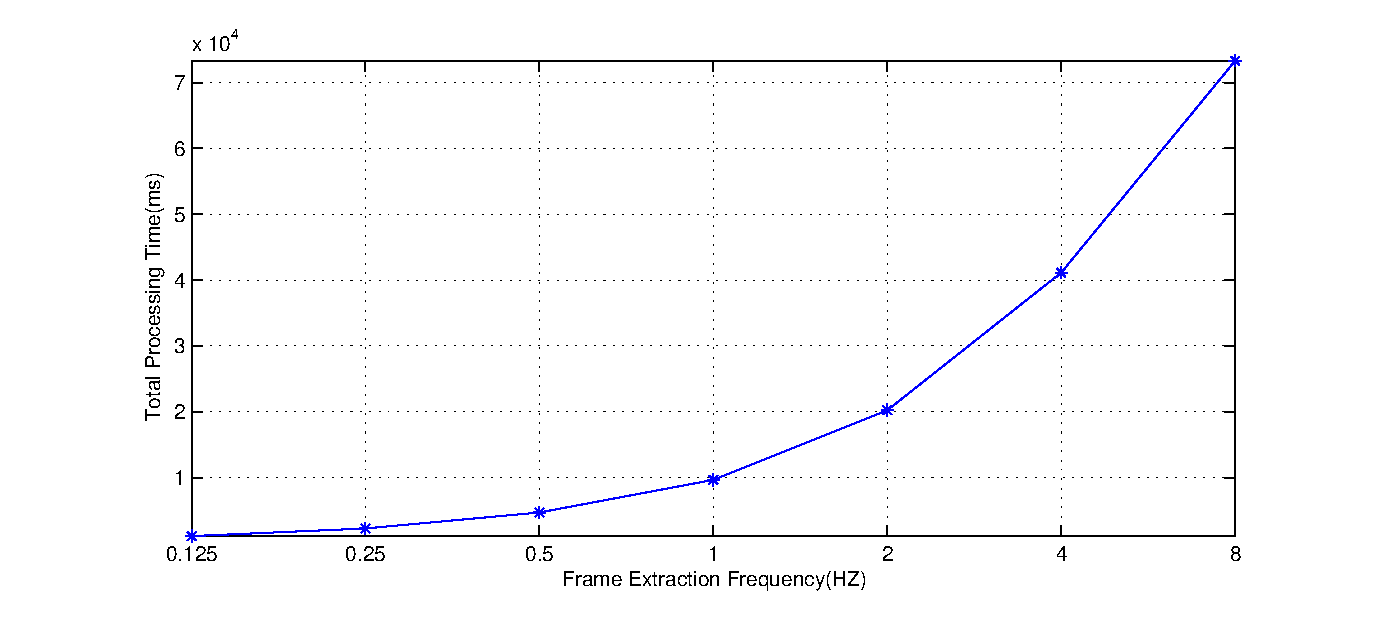
\includegraphics[width=2in]{pics/30s_frame.eps}\label{fig:3_1}}
%     \hfil
%     \subfigure[Average 60s Videos  Processing Time]{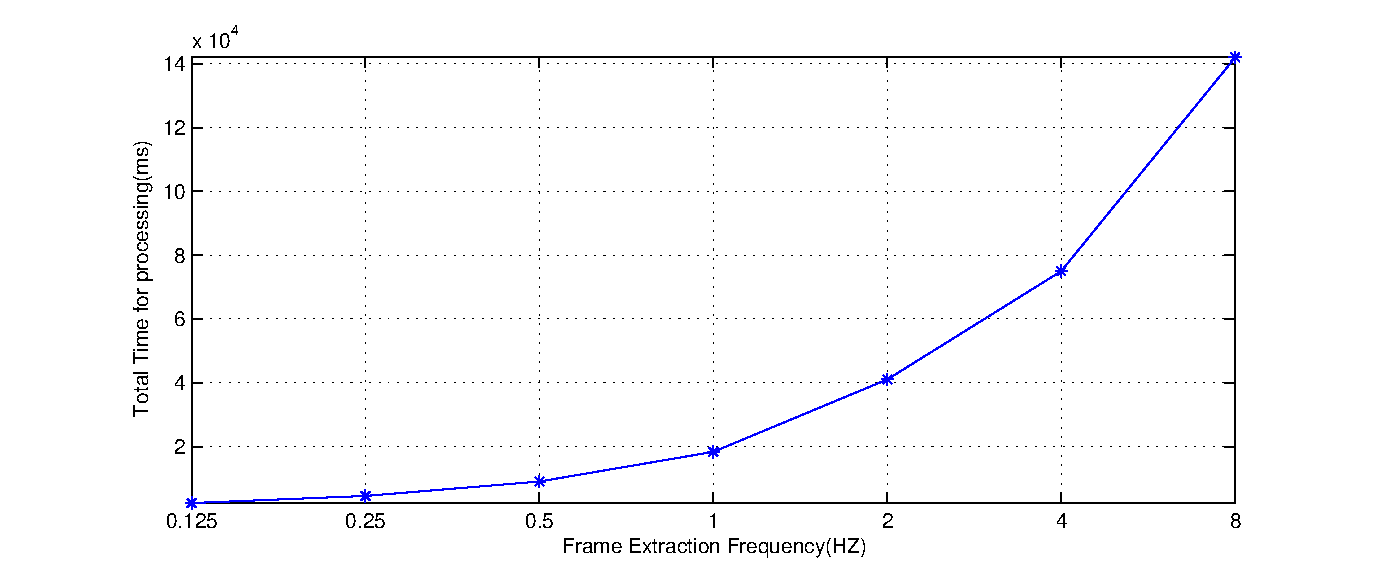
\includegraphics[width=2in]{pics/60s_frame.eps}\label{fig:3_2}}
%     \hfil
%     \subfigure[Average 120s Videos  Processing Time]{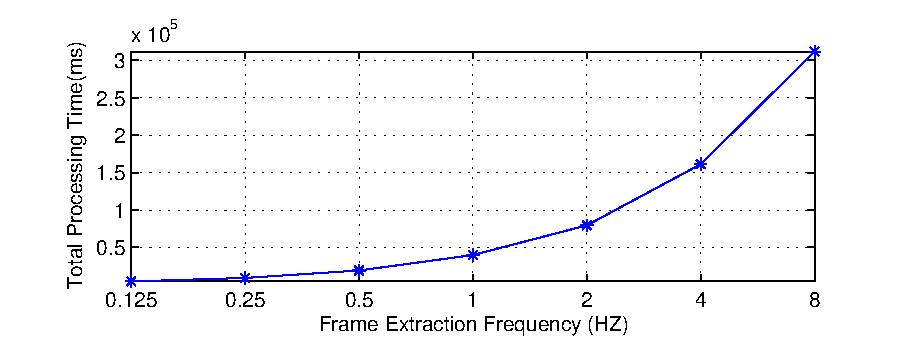
\includegraphics[width=2in]{pics/120s_frame.eps}\label{fig:3_3}}
% }
% \vspace{-1mm}
% \caption{Average Video Frame Extraction Time For Different Duration and Frequency}
% \vspace{-6mm}
% \label{fig:frame}
% \end{figure*}
%
% .
% \begin{enumerate}
%     \item Given a video, extract frames at different rate: 0.5Hz, 1Hz, 2Hz,... get the average extracting time for each rate
%     \item Fix a rate, extract different size video, see if there is any affects for different size video
% \end{enumerate}
% \subsubsection{Feature extraction}
% For the feature extraction of single image, we need to consider two aspects of cost, first, the cost of resizing, second, the cost of feature extraction of resized image. We use Galaxy SIII for this cost evaluation, we took about 300 photos of different kinds of scene with phone's own camera, and rescale them to different size, and record different component time for processing each file, and get the average time. We can see from the figure that...
% \begin{enumerate}
%    \item Given an image data base, resize all the images into  a fixed size. Do different feature extraction algorithm, and compare these algorithm's average extracting time
%    \item resize image data base into different size(100x100, 200x240, 300x400...), compare the average time for these sizes for different algorithm
% \end{enumerate}
%
% \subsubsection{Communication Measurement}
% End2End uploading speed estimate, give a uploading command from server and wait the end of file uploading, see the time. We vary
% the file size: a small photo to a large video. Compare WiFi(ENL WiFi) and cellular network (OPTIONAL: minus the real file uploading time from phone to server, we can see the overhead, how does the overhead vary?)
%
% \subsection {Background Media File Processing Performance}
% There might exists a scenario that media file process is running while  people are using their phones, we should ensure people's experience not much affected by our background processing.
%
% The experiment, we need to show the cpu and memory occupation by this thread.
%
% \subsection{Simpler System Comparison}
% Take away some part of our system, see how results perform;
%
% \subsection{Dynamic vs. Static Uploading Scheme}
% In fact, we have two kinds of scheme for file uploading, since the optimization result is sensitive, one way is to dynamically re-optimize and update the uploading list to phone, another is that push an enough long list to the phone and let phone do static uploading. The drawback of dynamic uploading is that the task assigning and killing process wastes a lot of resources, the results would be bad comparing to static uploading.
%
% We should show the reason why we choose static uploading finally
%
%
%
% \subsection{ Evaluation of  Concurrent Queries}
% \begin{enumerate}
% \item Set up and replay concurrent queries to compare with other uploading schemes: 1) round robin; 2) max credit first; 3) earliest deadline first;
% \item Compare to the ``optimal result'': run concurrent queries and record necessary parameters, use the information as facts in real world, apply scheme to get the ''Optimal Result''
% \end{enumerate}
%
% \subsection{Evaluating Overall Results}
% \begin{enumerate}
% \item Show the output performance with some intuitive metric;
% \item Compare with other possible phone media retrieval scheme;
% \end{enumerate}
%
% \subsection{Robustness and Scalability}
% \begin{enumerate}
% \item Handling burst of concurrent queries;
% \item Scales to \bf{N} phones, see how server performs, any degrading?
% \end{enumerate}


\vspace*{-1ex}
\section{Related Work}
\label{sec-5}

Perhaps the closest related piece of work to MediaScope is
CrowdSearch~\cite{crowdsearch}, which attempts to search for the
closest match image generated on a mobile device from among a set of
images stored on a photo sharing service.
%
Its focus, however, is complementary to MediaScope, and is on bridging
the semantic gap inherent in feature-based image searches; most
feature extraction methods do not understand the semantics of images,
and CrowdSearch focuses on using human intelligence in near real-time
to complete search tasks.
%
MediaScope can use this capability to filter search results to bridge
the semantic gap, but its focus is on supporting a richer query
interface and enabling tighter timeliness constraints than might be
possible with humans in the loop.

Also closely related is PhotoNet~\cite{photonet}, which
proposes an opportunistic image sharing and transmission capability in
a delay tolerant network.
%
PhotoNet uses similar image features to perform photo comparisons, but
is otherwise very different from MediaScope in that the latter
explicitly supports a query interface with timeliness constraints on queries.
% is a centralized system that metadata are
% aggregated to the server, avoid the peer-to-peer communication
% overhead.
%

MediaScope is informed and inspired by several pieces of work on
techniques for content-based image retrieval, and image search on
mobile devices.

In the former category are systems like Faceted Image Search
~\cite{faceted}, the Virage Image Search Engine~\cite{virage} and
ImgSeek~\cite{imgseek}, that support searches on a centralized
database of images.
%
\mscope builds upon these search techniques, but unlike them, supports
timely geometric queries over a distributed database of images and
videos on mobile devices.
%
Other work in content-based image retrieval has proposed
clustering~\cite{hierac,content4}, but has not explored the mobile
device setting.

% Moreover, these only support best match queries since they use
% similarity measures like the Tanimoto distance\cite{cedd,fuzzy} which
% does not correspond to a metric space.
% %
% \mscope builds upon these search techniques, but uses a metric
% distance and so can support timely geometric queries over a
% distributed database of images and videos on mobile devices.


% \cite{tinydb} proposed a query processor for sensor networks, compared with \mscope, sensor has much less processing power and less stable system than current advanced smart phones. Besides, MSMobile in \mscope also support multi-media processing that further abstract the data other than purely passive database.

A second category of work has explored support for image search on a
mobile device.
%
For example, ~\cite{energy} discusses energy efficient feature
extraction on a mobile device but supports on the local searches on
the device, as does~\cite{fast}.
%
Other pieces of work have explored a client/server architecture for
image search, but where the content is stored on the
server~\cite{content1,content2,content3}.
%
By contrast, \mscope supports searches on a cloud server, but where
the content is stored on the mobile devices and is retrieved on
demand.

Finally, tangentially related to MediaScope is work on automated or
semi-automated annotation of images with context obtained from sensors
~\cite{MMM2,PhotoMap,TagSense}.
%
MediaScope can use such annotations to support a broader range of
queries, but we have left this to future work.

% Another category of work is about image retrieval on mobile devices. In \cite{energy}, they have the similar idea of implementing CBIR algorithm on phone, they tried to improve the energy consumption for ImgSeek\cite{imgseek} by minimizing number of features for comparison on mobile phone, however, the heavier part of ImgSeek\cite{imgseek} is on feature extraction, but  \mscope moved the feature comparison part to cloud. Moreover, \cite{energy} only support local image search on phone, which turns out not useful compared to \mscope.  In \cite{fast}, authors also proposed a fast content retrieval scheme for mobile devices and support three different queries, compared with \mscope, their application is constrained on a single mobile phone, without information sharing, and their different queries are in fact the same scheme with traditional image search with feature extraction on different input images.   \cite{content1}\cite{content2}\cite{content3}  also introduce the image search with a cloud-client architecture, but it only uses phone as a client to search the content on the server.

% MMM2\cite{mmm2} is an early piece of work that aimed at lightweight photo sharing, however it needs to upload the images to a server that processes the image and returns metadata  for sharing, which is the way \mscope want to avoid(uploading to server)

% PhotoMap\cite{photomap} is another system that intends to provides  semi-automatic annotation about spatial related information of photos for mobile phones, which is already a usual characteristic of current smart phone. \mscope goes far beyond that, since \mscope automatically extract the photo and video features.



% In TagSense\cite{tagsense}, the authors described a system that tagging the people who appear in  photos by phone-to-phone communication, which needs all people runs the service. The CBIR tagging service in  \mscope is a more natural way in vision society, and \mscope also achieves the goal of automatic media file feature extraction, which overcomes their method.

% Finally, the queries we designed in \mscope are inspired by prior work. Clustering is widely used for content based image search\cite{hierac}\cite{content4}. \mscope provides a more high level conceptual search, which is not discussed before.

% \begin{itemize}
% \item Image Search
% \item UIUC related work, other mobile papers
% \end{itemize}

%\vspace*{-1ex}
\section{Conclusions}
\label{sec-6}

In this paper, we have discussed the MediaScope, a system that bridges
the availability gap for visual media by supporting timely on-demand
retrieval of images and video.
%
MediaScope uses a credit-based timeliness-aware scheduling algorithm
that optimizes query completeness, and its overheads are moderate.
%
\camera{Much work remains, including optimizing the internals of the
  system to improve completeness, and supporting more geometric
  queries on visual media.
%
  Larger scale experiments using more mobile devices can help
  understand how well the system scales, and how network variability
  can impact query completeness.
%
  Finally, a user study focused on understanding how well \mscope's
  query results bridge the semantic gap can help establish \mscope's
  usefulness.
%
}



%\vspace{2ex}
{
\footnotesize
\bibliographystyle{abbrv}
\bibliography{main}}

\end{document}
